% STOC 2027 review version: main argument with complete deferred proofs.
% Preparation notes and remaining editorial work: ../notes/stoc2027/
\documentclass[11pt,letterpaper]{article}
\usepackage[T1]{fontenc}
\usepackage[margin=1in]{geometry}
\usepackage{times}
\usepackage{amsmath,amssymb,amsthm,mathtools}
\usepackage{dsfont}
\allowdisplaybreaks
\raggedbottom
\usepackage{booktabs,graphicx,xcolor,microtype,tikz,needspace}
\usepackage{hyperref}
\usepackage[noabbrev,nameinlink]{cleveref}
\usepackage{lean_equation_links}
% Begin lean_listings.tex
\usepackage{listings}
\lstdefinestyle{lean}{
  basicstyle=\ttfamily\normalsize,
  columns=fullflexible,
  keepspaces=true,
  breaklines=true,
  breakatwhitespace=true,
  breakindent=1em,
  showstringspaces=false,
  aboveskip=\medskipamount,
  belowskip=\medskipamount,
  morekeywords={abbrev,def,noncomputable,structure,where,namespace,end,open,theorem},
  keywordstyle=\bfseries,
  literate=
    {ℝ}{{$\mathbb R$}}1
    {ℕ}{{$\mathbb N$}}1
    {ℚ}{{$\mathbb Q$}}1
    {∧}{{$\wedge$}}1
    {→}{{$\rightarrow$}}1
    {∀}{{$\forall$}}1
    {∃}{{$\exists$}}1
    {∑}{{$\textstyle\sum$}}1
    {⟨}{{$\langle$}}1
    {⟩}{{$\rangle$}}1
    {₁}{{$_1$}}1
    {₂}{{$_2$}}1
    {₃}{{$_3$}}1
    {⊆}{{$\subseteq$}}1
    {∪}{{$\cup$}}1
    {↑}{{$\uparrow$}}1
    {↥}{{$\Uparrow$}}1
    {⧸}{{$/$}}1
    {≤}{{$\leq$}}1
    {π}{{$\pi$}}1
    {σ}{{$\sigma$}}1
    {≃}{{$\simeq$}}1
    {≠}{{$\neq$}}1
    {∈}{{$\in$}}1
    {∉}{{$\notin$}}1
    {•}{{$\bullet$}}1
    {∅}{{$\varnothing$}}1
    {¬}{{$\neg$}}1
}
% End lean_listings.tex

\definecolor{leangray}{gray}{0.35}
\newcommand{\leanref}[3]{\href{\leanbase/#1\#L#2}{\textcolor{leangray}{\texttt{#3}}}}
\newcommand{\leanid}[3]{\leanref{#1}{#2}{lean\_#3}}
\newcommand{\leanlink}[3]{\leanref{#1}{#2}{#3}}
\newcounter{leanlinkno}
\newcommand{\lean}[2]{\stepcounter{leanlinkno}\leanref{#1}{#2}{Lean\_\theleanlinkno}}
\newcommand{\leandecl}[3]{\lean{#1}{#2}}
\newcommand{\leanlinkdecl}[4]{\leanlink{#1}{#2}{#4}}
% BEGIN GENERATED EQUATION LINKS
% Generated by scripts/paper_links.py; do not edit.
\makeatletter
\newcommand{\DeclareSourceEquation}[2]{\expandafter\def\csname paper@lean@#1\endcsname{#2}}
\makeatother
\newcommand{\leanbase}{https://github.com/JayPiZimmermann/Max\_Caterpillar/blob/039d68443bca6a324955031992db10b6e896f2d4}
\DeclareLeanEquation{eq:width}{MaxCaterpillar/Theorems.lean}{41}
\DeclareLeanEquation{eq:count}{MaxCaterpillar/Definitions.lean}{63}
\DeclareLeanEquation{eq:word}{MaxNN/Constructions/Paramid/Caterpillar/Corrections/Formula.lean}{130}
\DeclareLeanEquation{eq:faces}{MaxNN/Constructions/Paramid/Caterpillar/Corrections/Keys.lean}{29}
\DeclareLeanEquation{eq:face-description}{MaxNN/Constructions/Paramid/Caterpillar/Corrections/Keys.lean}{29}
\DeclareLeanEquation{eq:dictionary-span}{MaxCaterpillar/Lemmas.lean}{54}
\DeclareLeanEquation{eq:class-identity}{MaxCaterpillar/Lemmas.lean}{48}
\DeclareLeanEquation{stp:class}{MaxCaterpillar/Lemmas.lean}{48}
\DeclareLeanEquation{eq:geometric-class}{MaxNN/Constructions/Paramid/Geom/Faces/ConeOnly.lean}{71}
\DeclareLeanEquation{stp:corrections}{MaxNN/Constructions/Paramid/Geom/Faces/ConeOnly.lean}{71}
\DeclareLeanEquation{eq:coordinate-deletion}{MaxCaterpillar/Lemmas.lean}{41}
\DeclareLeanEquation{eq:insertion-weight-germs}{MaxNN/Constructions/Paramid/Caterpillar/Coordinate/Structured.lean}{67}
\DeclareLeanEquation{eq:graph}{MaxNN/Constructions/Paramid/Caterpillar/Corrections/Spine/GraphKey.lean}{214}
\DeclareLeanEquation{eq:cone-count}{MaxCaterpillar/Lemmas.lean}{66}
\DeclareLeanEquation{eq:features}{MaxNN/Constructions/Paramid/Caterpillar/Corrections/CompactFeatures.lean}{63}
\DeclareLeanEquation{eq:compilation-widths}{MaxCaterpillar/Retained.lean}{80}
\DeclareLeanEquation{stp:size-network}{MaxCaterpillar/Retained.lean}{80}
\DeclareLeanEquation{eq:network-parameters}{MaxCaterpillar/Definitions.lean}{29}
\DeclareLeanEquation{eq:network-evaluation}{MaxCaterpillar/Definitions.lean}{38}
\DeclareLeanEquation{eq:maximum}{MaxCaterpillar/Definitions.lean}{54}
\DeclareLeanEquation{eq:signed-word-sum}{MaxNN/Constructions/Paramid/Caterpillar/Formula/Values.lean}{31}
\DeclareLeanEquation{eq:hinging-maps}{MaxCaterpillar/CPWL.lean}{35}
\DeclareLeanEquation{eq:hinging-representation}{MaxCaterpillar/CPWL.lean}{35}
\DeclareLeanEquation{eq:max-hinge}{MaxNN/Core/Relu.lean}{24}
\DeclareLeanEquation{eq:caterpillar-data}{MaxNN/Constructions/Paramid/Caterpillar/Corrections/Formula.lean}{24}
\DeclareLeanEquation{eq:word-parent}{MaxNN/Constructions/Paramid/Caterpillar/Words.lean}{28}
\DeclareLeanEquation{eq:word-gamma}{MaxNN/Constructions/Paramid/Caterpillar/Corrections/Formula.lean}{122}
\DeclareLeanEquation{eq:edge-functions}{MaxNN/Constructions/Paramid/Caterpillar/Corrections/Formula.lean}{126}
\DeclareLeanEquation{eq:edge-comparison}{MaxNN/Constructions/Paramid/Caterpillar/Corrections/Formula.lean}{126}
\DeclareLeanEquation{eq:aux_functions}{MaxNN/Constructions/MaxN/Width/Layer/Features.lean}{75}
\DeclareLeanEquation{eq:hinge-reversal}{MaxNN/Core/Relu.lean}{33}
\DeclareLeanEquation{eq:remainder-translation}{MaxNN/Constructions/Paramid/Caterpillar/Corrections/CompactCovariance.lean}{74}
\DeclareLeanEquation{eq:simplex}{MaxNN/Constructions/Paramid/Geom/Defs.lean}{121}
\DeclareLeanEquation{eq:support-function}{MaxNN/Constructions/Paramid/Geom/Defs.lean}{43}
\DeclareLeanEquation{eq:unit-polytope}{MaxNN/Constructions/Paramid/Geom/Boundary/ConeFaces.lean}{400}
\DeclareLeanEquation{eq:exposed-face}{MaxNN/Constructions/Paramid/Geom/Defs.lean}{62}
\DeclareLeanEquation{eq:facet-difference}{MaxNN/Constructions/Paramid/Geom/Germ.lean}{460}
\DeclareLeanEquation{eq:face-derivative}{MaxNN/Constructions/Paramid/Geom/Germ.lean}{364}
\DeclareLeanEquation{eq:facet-error}{MaxNN/Constructions/Paramid/Caterpillar/Corrections/Formula.lean}{184}
\DeclareLeanEquation{eq:linear-facet}{MaxNN/Constructions/Paramid/Caterpillar/Formula/Braid.lean}{96}
\DeclareLeanEquation{eq:lifted-induction}{MaxNN/Constructions/Paramid/Caterpillar/Formula/Lift.lean}{40}
\DeclareLeanEquation{eq:induction-error-split}{MaxNN/Constructions/Paramid/Caterpillar/Formula/Assembly.lean}{69}
\DeclareLeanEquation{eq:root-star}{MaxNN/Constructions/Paramid/Caterpillar/Coordinate/Star.lean}{25}
\DeclareLeanEquation{eq:boolean-cancellation}{MaxNN/Constructions/Paramid/Caterpillar/Words/RootStar.lean}{47}
\DeclareLeanEquation{eq:full-coordinates}{MaxNN/Constructions/Paramid/Geom/Coordinates.lean}{27}
\DeclareLeanEquation{eq:head-count-bound}{MaxCaterpillar/Asymptotics.lean}{31}
\DeclareLeanEquation{eq:cone-growth}{MaxCaterpillar/Asymptotics.lean}{44}
\DeclareLeanEquation{eq:second-growth}{MaxCaterpillar/Asymptotics.lean}{54}
\DeclareLeanEquation{eq:first-growth}{MaxCaterpillar/Asymptotics.lean}{17}
\DeclareLeanEquation{eq:absorbed-pairs}{MaxNN/Constructions/Paramid/Caterpillar/Corrections/AbsorbHinges.lean}{26}
\DeclareLeanEquation{eq:recover-coordinates}{MaxNN/Constructions/Paramid/Caterpillar/Corrections/CompactFeatures.lean}{111}
\DeclareLeanEquation{eq:feature-count}{MaxNN/Constructions/Paramid/Caterpillar/Corrections/CompactFeatures.lean}{21}
\DeclareLeanEquation{eq:normalized-description}{MaxNN/Constructions/Paramid/Caterpillar/Corrections/Normalize.lean}{24}
\DeclareLeanEquation{eq:facet-reduction}{MaxCaterpillar/Lemmas.lean}{33}
\DeclareLeanEquation{stp:reconstruction}{MaxCaterpillar/Lemmas.lean}{33}
\DeclareLeanEquation{eq:base-unit}{MaxNN/Constructions/Paramid/Caterpillar/Coordinate/Base.lean}{78}
\DeclareLeanEquation{eq:base-formula}{MaxNN/Constructions/Paramid/Caterpillar/Coordinate/Base.lean}{84}
\DeclareLeanEquation{eq:simplex-facet}{MaxNN/Constructions/Paramid/Caterpillar/Formula/SimplexGerms.lean}{60}
\DeclareLeanEquation{eq:kuhn-simplices}{MaxNN/Constructions/Paramid/Geom/Kuhn.lean}{43}
\DeclareLeanEquation{eq:kuhn-support-error}{MaxNN/Constructions/Paramid/Geom/Kuhn.lean}{320}
\DeclareLeanEquation{eq:apex-maximum}{MaxNN/Constructions/Paramid/Caterpillar/Geometry/Paramid.lean}{43}
\DeclareLeanEquation{eq:retained-count}{MaxCaterpillar/Retained.lean}{80}
\DeclareLeanEquation{stp:size-count}{MaxCaterpillar/Retained.lean}{80}
\DeclareLeanEquation{eq:face-dimension-drop}{MaxNN/Constructions/Paramid/Geom/Flag.lean}{200}
\DeclareLeanEquation{eq:error-peeling}{MaxNN/Constructions/Paramid/Geom/Faces/Peel.lean}{38}
\DeclareLeanEquation{eq:simplex-vertex-removal}{MaxNN/Constructions/Paramid/Geom/Faces/ConeOnly/SimplexGerm.lean}{184}
\DeclareLeanEquation{eq:initial-simplex-error}{MaxNN/Constructions/Paramid/Geom/Faces/ConeOnly/LocalIdentity.lean}{205}
\DeclareLeanEquation{eq:simplex-deletion-sign}{MaxNN/Constructions/Paramid/Geom/Faces/ConeOnly/SimplexGerm.lean}{195}
\DeclareLeanEquation{eq:simplex-induction-use}{MaxNN/Constructions/Paramid/Geom/Faces/ConeOnly.lean}{40}
\DeclareLeanEquation{eq:residual-invariant}{MaxNN/Constructions/Paramid/Geom/Faces.lean}{69}
\DeclareLeanEquation{eq:support-cut}{MaxNN/Constructions/Paramid/Geom/Sweep/Support.lean}{142}
\DeclareLeanEquation{eq:sweep-support-high}{MaxNN/Constructions/Paramid/Geom/Sweep.lean}{187}
\DeclareLeanEquation{eq:sweep-support-translate}{MaxNN/Constructions/Paramid/Geom/Sweep.lean}{304}
\DeclareLeanEquation{eq:sweep-operation}{MaxNN/Constructions/Paramid/Geom/Defs.lean}{106}
\DeclareLeanEquation{eq:sweep-dimension}{MaxNN/Constructions/Paramid/Geom/Sweep.lean}{366}
\DeclareLeanEquation{eq:simplex-reconstruction}{MaxNN/Constructions/Paramid/Geom/Reconstruct.lean}{83}
\DeclareLeanEquation{eq:simplex-isolate-facet}{MaxNN/Constructions/Paramid/Geom/Reconstruct/FacetGerm.lean}{268}
\DeclareLeanEquation{eq:normalized-facet-normal}{MaxNN/Constructions/Paramid/Geom/Reconstruct/FacetGerm.lean}{185}
\DeclareLeanEquation{eq:facet-group-bound}{MaxNN/Constructions/Paramid/Geom/Reconstruct/FacetGerm.lean}{326}
\DeclareLeanEquation{eq:single-facet-group}{MaxNN/Constructions/Paramid/Geom/Reconstruct/FacetGerm.lean}{326}
\DeclareLeanEquation{eq:translation-invariance}{MaxNN/Constructions/Paramid/Caterpillar/Corrections/CompactCanonical.lean}{22}
\DeclareLeanEquation{eq:retained-descriptions}{MaxCaterpillar/Retained.lean}{31}
\DeclareLeanEquation{eq:ridge-cut-residual}{MaxNN/Constructions/Paramid/Geom/Reconstruct/SimplexCut.lean}{613}
\DeclareLeanEquation{eq:simplex-support-expansion}{MaxNN/Constructions/Paramid/Caterpillar/Formula/Completeness.lean}{80}
\DeclareLeanEquation{eq:direction-pattern-spine}{MaxNN/Constructions/Paramid/Caterpillar/Geometry/Facets/Pattern.lean}{64}
\DeclareLeanEquation{eq:direction-pattern}{MaxNN/Constructions/Paramid/Caterpillar/Geometry/Facets/Pattern.lean}{64}
\DeclareLeanEquation{eq:braid-reflection}{MaxNN/Constructions/Paramid/Caterpillar/Formula/Braid.lean}{66}
\DeclareLeanEquation{eq:braid-germ}{MaxNN/Constructions/Paramid/Geom/Germ/Reflection.lean}{34}
\DeclareLeanEquation{eq:block-pairing}{MaxNN/Constructions/Paramid/Caterpillar/Geometry/Toggle.lean}{42}
\DeclareLeanEquation{eq:lower-arity-translation}{MaxNN/Constructions/Paramid/Caterpillar/Formula/Lift.lean}{30}
\DeclareLeanEquation{eq:coordinate-active}{MaxNN/Constructions/Paramid/Caterpillar/Coordinate/Active.lean}{20}
\DeclareLeanEquation{eq:coordinate-fibre-partition}{MaxNN/Constructions/Paramid/Caterpillar/Coordinate/ReindexActive.lean}{228}
\DeclareLeanEquation{eq:root-star-average}{MaxNN/Constructions/Paramid/Caterpillar/Coordinate/Star.lean}{315}
\DeclareLeanEquation{eq:lower-caterpillar-summand}{MaxNN/Constructions/Paramid/Caterpillar/Coordinate/Structured.lean}{23}
\DeclareLeanEquation{eq:auxiliary-remainder}{MaxNN/Constructions/Paramid/Caterpillar/Corrections/CompactCovariance.lean}{22}
\DeclareLeanEquation{eq:compact-remainder}{MaxNN/Constructions/Paramid/Caterpillar/Corrections/CompactCovariance.lean}{89}
\DeclareLeanEquation{eq:network-assembly}{MaxCaterpillar/Construction.lean}{39}
\DeclareLeanEquation{eq:signed-remainder}{MaxNN/Constructions/Paramid/Caterpillar/Corrections/CompactCanonical.lean}{57}
\DeclareLeanEquation{eq:coordinate-relabel}{MaxNN/Constructions/Paramid/Caterpillar/Formula/CoordinateDirections.lean}{119}
\DeclareLeanEquation{eq:compilation-hypothesis}{MaxCaterpillar/Core.lean}{30}
\DeclareLeanEquation{eq:rational-coordinate}{MaxCaterpillar/Rationality.lean}{64}
\DeclareLeanEquation{eq:quotient-dimension}{MaxCaterpillar/Quotient.lean}{44}
\DeclareLeanEquation{eq:quotient-width}{MaxCaterpillar/Quotient.lean}{57}
\DeclareLeanEquation{eq:max-three}{MaxCaterpillar/SmallArity.lean}{62}
\DeclareLeanEquation{eq:max-four}{MaxCaterpillar/SmallArity.lean}{117}
\DeclareLeanEquation{eq:kmps}{MaxCaterpillar/KMPS.lean}{410}
\DeclareLeanEquation{eq:count-binomial}{MaxCaterpillar/Theorems.lean}{113}
\DeclareLeanEquation{eq:count-exponential}{MaxCaterpillar/Theorems.lean}{121}
\DeclareLeanEquation{eq:count-quadratic}{MaxCaterpillar/Theorems.lean}{155}
\DeclareLeanEquation{eq:base-point}{MaxCaterpillar/Count/Locality.lean}{39}
\DeclareLeanEquation{eq:mixed-difference}{MaxCaterpillar/Count/Locality.lean}{53}
\DeclareLeanEquation{eq:balanced}{MaxCaterpillar/Count/Locality.lean}{82}
\DeclareLeanEquation{eq:active}{MaxCaterpillar/Count/Locality.lean}{88}
\DeclareLeanEquation{eq:mixed-auxiliary}{MaxCaterpillar/Count/Locality.lean}{263}
\DeclareLeanEquation{stp:count-functional}{MaxCaterpillar/Count/Locality.lean}{263}
\DeclareLeanEquation{eq:mixed-maximum}{MaxCaterpillar/Count/Locality.lean}{280}
\DeclareLeanEquation{eq:preactivation-digits}{MaxCaterpillar/Count/Passing.lean}{198}
\DeclareLeanEquation{stp:count-digits}{MaxCaterpillar/Count/Passing.lean}{198}
\DeclareLeanEquation{stp:count-admissible}{MaxCaterpillar/Count/PerUnit.lean}{172}
\DeclareLeanEquation{eq:order-count}{MaxCaterpillar/Count/Passing.lean}{541}
\DeclareLeanEquation{stp:count-orders}{MaxCaterpillar/Count/Passing.lean}{541}
\DeclareLeanEquation{eq:path-weight}{MaxCaterpillar/Count/PerUnit.lean}{211}
\DeclareLeanEquation{stp:count-transfer}{MaxCaterpillar/Count/PerUnit.lean}{211}
\DeclareLeanEquation{eq:binomial-sum}{MaxCaterpillar/Count/Main.lean}{69}
\DeclareLeanEquation{stp:count-corollary}{MaxCaterpillar/Count/Main.lean}{69}
\DeclareLeanEquation{stp:quotient-independence}{MaxCaterpillar/Dimension.lean}{379}
\DeclareLeanEquation{eq:path-unit}{MaxCaterpillar/Dimension.lean}{177}
\DeclareLeanEquation{stp:quotient-path-units}{MaxCaterpillar/Dimension.lean}{177}
\DeclareLeanEquation{eq:test-configuration}{MaxCaterpillar/Dimension.lean}{241}
\DeclareLeanEquation{stp:quotient-auxiliary}{MaxCaterpillar/Dimension.lean}{92}
\DeclareLeanEquation{eq:path-functional}{MaxCaterpillar/Dimension.lean}{278}
\DeclareLeanEquation{stp:quotient-path-values}{MaxCaterpillar/Dimension.lean}{278}
\DeclareLeanEquation{eq:bsy-hyperplane}{MaxCaterpillar/Competing/Defs.lean}{68}
\DeclareLeanEquation{eq:bsy-parallelepiped}{MaxCaterpillar/Competing/Defs.lean}{78}
\DeclareLeanEquation{eq:bsy-marked}{MaxCaterpillar/Competing/Defs.lean}{99}
\DeclareLeanEquation{eq:rooted-star}{MaxCaterpillar/Competing/Defs.lean}{121}
\DeclareLeanEquation{eq:bsy-zonotope}{MaxCaterpillar/Theorems.lean}{203}
\DeclareLeanEquation{eq:bsy-support}{MaxCaterpillar/Theorems.lean}{231}
\DeclareLeanEquation{eq:bsy-word}{MaxCaterpillar/Theorems.lean}{240}
\DeclareLeanEquation{stp:bsy-coordinates}{MaxCaterpillar/Competing/Relation.lean}{320}
\DeclareLeanEquation{stp:bsy-injective}{MaxCaterpillar/Competing/Relation.lean}{331}
\DeclareLeanEquation{stp:bsy-zonotope}{MaxCaterpillar/Competing/Relation.lean}{391}
\DeclareLeanEquation{stp:bsy-support}{MaxCaterpillar/Competing/Support.lean}{55}
\DeclareLeanEquation{stp:bsy-word}{MaxCaterpillar/Competing/Support.lean}{238}
\DeclareLeanEquation{stp:bsy-star}{MaxCaterpillar/Competing/Support.lean}{454}
\DeclareLeanEquation{eq:forest-count}{MaxCaterpillar/Count/Main.lean}{26}
\DeclareLeanEquation{stp:count-assembly}{MaxCaterpillar/Count/Main.lean}{26}
\DeclareLeanEquation{eq:block-weight}{MaxCaterpillar/Count/BlockSum.lean}{95}
\DeclareSourceEquation{eq:fixed-five-features}{https://github.com/JayPiZimmermann/Max\_Caterpillar/blob/b5615d0745f8b064dc6ee374c6ae584a0957bc10/research/sN/best5/netB\_10\_6.json}
\DeclareSourceEquation{eq:fixed-five-identity}{https://github.com/JayPiZimmermann/Max\_Caterpillar/blob/b5615d0745f8b064dc6ee374c6ae584a0957bc10/research/sN/best5/netB\_10\_6.json}
\DeclareSourceEquation{eq:fixed-five-scalar}{https://github.com/JayPiZimmermann/Max\_Caterpillar/blob/b5615d0745f8b064dc6ee374c6ae584a0957bc10/research/sN/best5/netB\_10\_6.json}
\DeclareSourceEquation{eq:fixed-five-free}{https://github.com/JayPiZimmermann/Max\_Caterpillar/blob/b5615d0745f8b064dc6ee374c6ae584a0957bc10/research/sN/best5/overnight\_fixed\_bowtie.md\#reduction-to-four-free-neurons}
\DeclareSourceEquation{eq:fixed-five-translation}{https://github.com/JayPiZimmermann/Max\_Caterpillar/blob/b5615d0745f8b064dc6ee374c6ae584a0957bc10/research/sN/best5/overnight\_fixed\_bowtie.md\#reduction-to-four-free-neurons}
\DeclareSourceEquation{eq:fixed-five-difference}{https://github.com/JayPiZimmermann/Max\_Caterpillar/blob/b5615d0745f8b064dc6ee374c6ae584a0957bc10/research/sN/best5/overnight\_fixed\_bowtie\_verify.py}
\DeclareSourceEquation{eq:fixed-five-locality}{https://github.com/JayPiZimmermann/Max\_Caterpillar/blob/b5615d0745f8b064dc6ee374c6ae584a0957bc10/research/sN/best5/overnight\_fixed\_bowtie\_verify.py}
\DeclareSourceEquation{eq:degree-two-unit}{https://github.com/JayPiZimmermann/Max\_Caterpillar/blob/3ef5d3f673b8b31572155490711343017b6aa3f0/research/sN/trees/overnight\_degree\_two.md}
\DeclareSourceEquation{eq:degree-two-count}{https://github.com/JayPiZimmermann/Max\_Caterpillar/blob/3ef5d3f673b8b31572155490711343017b6aa3f0/research/sN/trees/overnight\_degree\_two.md}
\DeclareSourceEquation{eq:degree-two-capacity}{https://github.com/JayPiZimmermann/Max\_Caterpillar/blob/3ef5d3f673b8b31572155490711343017b6aa3f0/research/sN/trees/overnight\_degree\_two.md}
\DeclareSourceEquation{eq:fixed-five-rays}{https://github.com/JayPiZimmermann/Max\_Caterpillar/blob/b5615d0745f8b064dc6ee374c6ae584a0957bc10/research/sN/best5/overnight\_fixed\_bowtie\_pairs.md}
\DeclareSourceEquation{eq:weighted-forest-count}{https://github.com/JayPiZimmermann/Max\_Caterpillar/blob/4c9fbe4f63066e44d1f68bc184edc929d00a937b/research/sN/trees/overnight\_pseudoforest\_matching.md}
\DeclareSourceEquation{eq:matching-witnesses}{https://github.com/JayPiZimmermann/Max\_Caterpillar/blob/4c9fbe4f63066e44d1f68bc184edc929d00a937b/research/sN/trees/overnight\_pseudoforest\_matching.md}
\DeclareSourceEquation{eq:bounded-excess-count}{https://github.com/JayPiZimmermann/Max\_Caterpillar/blob/61b26cf955427ab7fbc6919a51623c98fded4740/research/sN/trees/overnight\_bounded\_excess.md}
\DeclareSourceEquation{eq:weighted-isolates}{https://github.com/JayPiZimmermann/Max\_Caterpillar/blob/6bd6f73902686fae54968dc339b92fa94fdbbd59/research/sN/trees/overnight\_read\_degree.md}
\makeatletter
\AtBeginDocument{%
\let\paper@linked@tagform\tagform@
\def\tagform@#1{%
\ifpaper@displaytag
\ifmeasuring@\else
\ifcsname paper@lean@\paper@equationlabel\endcsname\else
\PackageError{caterpillar}{Missing source link for equation `\paper@equationlabel'}{Run scripts/paper_links.py and copy the updated main.tex.}%
\fi
\fi
\fi
\paper@linked@tagform{#1}%
}%
}
\makeatother
% END GENERATED EQUATION LINKS

\newcommand{\fixedfivebase}{https://github.com/JayPiZimmermann/Max\_Caterpillar/blob/b5615d0745f8b064dc6ee374c6ae584a0957bc10/research/sN/best5}

\newtheorem{theorem}{Theorem}
\newtheorem*{representationtheorem}{Theorem}
\newtheorem*{depthconjecture}{Historical conjecture}
\newtheorem{lemma}[theorem]{Lemma}
\theoremstyle{definition}
\newtheorem{definition}[theorem]{Definition}
% Begin proof_commands.tex
% Structured proof commands adapted from arXiv:2610.01728v2.
\usepackage{refcount}
\newcommand{\pfnum}{??}
\newcounter{pfclaim}\newcounter{pfstep}
\newcounter{pfblock}
\renewcommand{\thepfclaim}{\pfnum.\arabic{pfclaim}}
\renewcommand{\thepfstep}{\pfnum.\arabic{pfstep}}
\providecommand{\theHpfclaim}{}
\providecommand{\theHpfstep}{}
\renewcommand{\theHpfclaim}{\arabic{pfblock}.\arabic{pfclaim}}
\renewcommand{\theHpfstep}{\arabic{pfblock}.\arabic{pfstep}}
\newenvironment{Proof}[2]{%
  \stepcounter{pfblock}%
  \setcounter{pfclaim}{0}\setcounter{pfstep}{0}%
  \xdef\pfnum{\getrefnumber{#2}}%
  \par\phantomsection\label[proof]{pf:#2}%
  \begin{proof}[\normalfont\bfseries Proof of \Cref{#2}]%
}{\end{proof}}
\newenvironment{ProofSketch}[2]{%
  \stepcounter{pfblock}%
  \setcounter{pfclaim}{0}\setcounter{pfstep}{0}%
  \xdef\pfnum{\getrefnumber{#2}}%
  \par\phantomsection\label[proof]{pf:#2}%
  \begin{proof}[\normalfont\bfseries Proof ideas of \Cref{#2}]%
}{\end{proof}}
\newcommand{\pfclaim}[2]{\par\medskip\refstepcounter{pfclaim}%
  \noindent\textbf{Claim \thepfclaim\ [#2].}\label{#1}\enspace\ignorespaces}
\newcommand{\pfstep}[2]{\par\medskip\refstepcounter{pfstep}%
  \noindent\textbf{\LeanLinkIfDeclared{#1}{Step \thepfstep}\ (#2).}\label{#1}\enspace\ignorespaces}
\newcommand{\finishes}[2]{This finishes the proof of \Cref{#2}.}
\newenvironment{Claim}[2]{%
  \pfclaim{#1}{#2}\itshape\ignorespaces}%
 {\par}
\newenvironment{ProofOf}[2]{%
  \vspace{-0.4\baselineskip}%
  \par\phantomsection\label[proof]{pf:#2}%
  \begin{proof}[\normalfont\bfseries Proof of \Cref{#2}]}%
 {\end{proof}}

% Cross-reference names for structured proof counters and proof destinations.
\crefname{pfclaim}{claim}{claims}
\Crefname{pfclaim}{Claim}{Claims}
\crefname{pfstep}{step}{steps}
\Crefname{pfstep}{Step}{Steps}
\crefname{proof}{proof}{proofs}
\Crefname{proof}{Proof}{Proofs}
\crefformat{proof}{#2proof#3}
\Crefformat{proof}{#2Proof#3}
\crefformat{aimethod}{#2AI methodology statement#3}
\Crefformat{aimethod}{#2AI methodology statement#3}
% End proof_commands.tex
\newcommand{\R}{\mathbb R}
\newcommand{\maxn}{\operatorname{max}}
\newcommand{\relu}{\sigma}
\newcommand{\spn}{\operatorname{span}}
\newcommand{\LS}{\mathcal L}
\newcommand{\D}{\mathcal D}
\newcommand{\B}{\mathcal B}
\newcommand{\one}{\mathbf 1}
\title{Two Hidden Layers Suffice: The Caterpillar Net}
\author{Jakob Paul Zimmermann\\
\normalfont FU Berlin, TU Berlin\\
\href{mailto:jakob.paul.zimmermann@campus.tu-berlin.de}{jakob.paul.zimmermann@campus.tu-berlin.de}\\
\url{https://jakob-paul-zimmermann.com}}
\date{}
\hypersetup{hidelinks,pdftitle={TWO HIDDEN LAYERS SUFFICE: THE CATERPILLAR NET},
  pdfauthor={Jakob Paul Zimmermann}}

\begin{document}
\hypersetup{pageanchor=false}
\maketitle
\thispagestyle{empty}
\begin{abstract}
\normalsize
Every continuous piecewise linear (CPWL) function is a finite signed sum of maxima of affine functions, making maximum representation a central problem in the study of the expressiveness of ReLU networks. Earlier work disproved the conjectured base-two depth bound, leaving open whether a constant number of hidden layers suffices to represent the maximum. Independently and concurrently, Brunck, Hertrich, Rue{\ss}, Stade, and Yehudayoff established that two hidden layers suffice for all CPWL functions.
We give the \emph{Caterpillar Net}, a non-recursive explicit construction representing the maximum of $N$ real inputs exactly with two hidden layers of widths $\binom N2+N+1$ and $2^{O(N\log N)}$, rational weights, and zero biases. Every expansion of the maximum in its finite vocabulary compiles with the same first hidden layer. Sharing its first hidden layer across a Wang--Sun representation gives two-hidden-layer networks for all CPWL functions.
\footnote{Our results were obtained over months of proof search in Lean using Claude Code and Codex; the AI methodology statement describes their roles. The Lean code is available in the accompanying repository \href{https://github.com/JayPiZimmermann/Max_Caterpillar}{https://github.com/JayPiZimmermann/Max\_Caterpillar}. Links to the Lean formalization appear in theorem titles and equation numbers; equation numbers are clickable.}
\end{abstract}
\setcounter{page}{1}
\hypersetup{pageanchor=true}

\section{Introduction}

In this paper we investigate the representation capabilities of ReLU
networks: what functions are representable by such networks of different
depths and widths? ReLU networks represent precisely the continuous
piecewise-linear (CPWL) functions with finitely many pieces
\cite{AroraEtAl}. A sharp question is therefore: given a CPWL function,
what is the smallest depth, or the smallest width at a prescribed depth,
needed to represent it exactly \cite{HertrichEtAl,SafranDepth}?
The maximum is a universal building block for such functions:
every CPWL function is a finite signed sum of maxima of affine
functions \cite{WangSun}. Write
\begin{align}\label{eq:maximum}
 \maxn_N(x):=\max_{0\leq i<N}x_i.
\end{align}

\begin{representationtheorem}[Wang--Sun, \cite{WangSun}, \leandecl{MaxCaterpillar/CPWL.lean}{35}{wang_sun}]
Let $d\geq1$ and let $f:\R^d\to\R$ be continuous and affine on each member
of a finite polyhedral cover. There are $R\in\mathbb N$, affine maps and signs
\begin{align}\label{eq:hinging-maps}
 A_t:\R^d\longrightarrow\R^{d+1},\qquad
 \varepsilon_t\in\{-1,1\}\qquad(1\leq t\leq R)
\end{align}
such that
\begin{align}\label{eq:hinging-representation}
 f(x)=\sum_{t=1}^R\varepsilon_t\maxn_{d+1}(A_t(x))
 \qquad\text{for every }x\in\R^d.
\end{align}
\end{representationtheorem}

Thus a two-hidden-layer representation of $\maxn_{d+1}$ gives one for every
CPWL function on $\R^d$: precompose with the affine maps and add the networks
in parallel. \Cref{sec:sharing} reuses their first hidden layer; the
representation theorems and the resulting networks are formalized.

\paragraph{Our contribution.}
The \emph{Caterpillar Net} gives a nonrecursive two-hidden-layer representation of the maximum with explicit bounds on both hidden-layer widths. The construction uses a finite dictionary of support functions of caterpillar polytopes and their faces. 
The maximum is the support function of a simplex. We first express this support function as an alternating sum of caterpillar support functions, up to a linear combination of support functions of lower-dimensional polytopes. We then represent the remaining error using faces of the same caterpillar polytopes and elementary ReLU features. Normalizing and merging these descriptions yields a width bound for the complete network, including all correction terms.

\Needspace{8\baselineskip}
Write $\relu(t):=\max(0,t)$ applied coordinatewise to vectors.
A network has an input layer of $N$ coordinates, first and second hidden
layers of widths $h_1$ and $h_2$, respectively, and a scalar output layer.
With real weight matrices $W_1,W_2$, output vector $w_3$, and biases
$b_1,b_2,b_3$ of the corresponding dimensions, it evaluates as
\begin{align}\label{eq:network-evaluation}
 x\longmapsto w_3^\top\relu\bigl(W_2\relu(W_1x+b_1)+b_2\bigr)+b_3.
\end{align}
There are no skip connections; equality is required on all of $\R^N$. For $N=1,2,3$ there are known simple network representations of width $(2,2)$ and $(4,2)$ and $(5,3)$; the last nests $\max(s,t)=t+\relu(s-t)$. Our Main Theorem presents such constructions for higher $N$.
A network has \emph{rational weights} if every entry of $W_1$, $W_2$, and $w_3$
is rational, and \emph{zero biases} if $b_1$, $b_2$, and $b_3$ vanish.

\Needspace{10\baselineskip}
\begin{theorem}[Caterpillar Net, \leandecl{MaxCaterpillar/Theorems.lean}{41}{caterpillar_net}, {\Cref{pf:thm:main}}]\label{thm:main}
For every $N\geq3$, there is a two-hidden-layer ReLU network with rational weights and zero biases computing $\maxn_N$ with widths
\begin{align}
 h_1=\binom N2+N+1,\qquad h_2=3^{N-2}C_N-N(N-1)+2,\label{eq:width}
\end{align}
where
\begin{align}\label{eq:count}
 C_N:=\sum_{m=2}^{N-1}\binom Nm\frac{m!}{2}(N-m)m^{N-m-1}.
\end{align}
Thus $h_1=O(N^2)$ and $h_2=2^{O(N\log N)}$ as $N\to\infty$.
\end{theorem}

\paragraph{Further results.}
The network is compiled from an expansion of $\maxn_N$ in a finite vocabulary
of caterpillar face functions. \Cref{thm:compilation} separates the network
from the coefficients: any such expansion with $|K|$ retained units compiles
with the same first hidden layer and $|K|+2$ second hidden layer neurons.
The coefficients are the coordinates of $\maxn_N$ in one basis of the
vocabulary; the same proof shows that they are rational, without any
integral (\Cref{thm:quotient-compression}).
\Cref{sec:compression} bounds the second width by $q_N+2$, where $q_N$ is the
dimension of the vocabulary modulo its auxiliary functions; this bound
proves \Cref{thm:main}. For $N=3,4$ expansions with one and three units are
proved in Lean. Conversely, \Cref{sec:lower} proves that every expansion of
$\maxn_N$ in caterpillar and auxiliary functions has at least
$(7/6)^N/(N+1)$ caterpillar functions, and that $q_N\geq(N-2)!$.
\Cref{sec:sharing} applies the
construction to sums of maxima.

\section{Related work}\label{sec:related}

The conjecture that $\max\{0,x_1,\ldots,x_{2^k}\}$ requires more than $k$
hidden layers \cite{HertrichEtAl} was disproved for $k=2$ by the maximum
of five inputs in \cite{BakaevEtAl}. Exact
computer-assisted searches subsequently obtained two-hidden-layer
representations up to $N=12$ in \cite{RuessEtAl} and, independently,
up to $N=8$ in \cite{WangBasu}. The improved general depth bounds remained
logarithmic, leaving constant depth open.

Setting all biases to zero does not change a network that computes a
positively homogeneous function such as $\maxn_N$
\cite[Proposition~2.3]{HertrichEtAl}, \cite[Lemma~7]{HaaseEtAl}, so biases
give no additional power for representing the maximum.
Depth lower bounds hold for integer weights \cite{HaaseEtAl} and rational
weights whose denominators are restricted to powers of a fixed integer
\cite{AverkovEtAl}. Our weights are rational, but their denominators are not
restricted in this way, so neither bound applies. Other
results concern braid-fan-compatible networks \cite{GrilloEtAl} and first
hidden layer width bounds \cite{SafranDepth,LuClosure}.

\begin{theorem}[Brunck, Hertrich, Rue{\ss}, Stade, and Yehudayoff, \cite{BSY}]\label{thm:bsy}
Every continuous piecewise affine function $f:\R^d\to\R$ with finitely
many affine pieces can be represented exactly by a ReLU network with two
hidden layers.
\end{theorem}
Their first proof proceeds by induction on dimension, using homological algebra to construct a linear combination of support functions of pyramids over zonotopes that agrees with the simplex support function modulo lower-dimensional terms. Our construction restricts these building blocks to an explicitly specified finite family, the caterpillar polytopes; we deliver a geometric proof of the corresponding identity.

Independently and concurrently, they developed a second proof based on combinatorial cancellation, with building blocks closely related to ours. \Cref{app:bsy} identifies them exactly: for nonempty marked sets their pyramids are translated caterpillar polytopes, and the remaining pyramids are rooted stars, which are not caterpillar functions. We do not claim that their coefficients agree with ours. We establish explicit width bounds for the first and second hidden layers; their paper states no widths.


\section{The Caterpillar Net}\label{sec:construction}

Two identities drive the construction:
\begin{align}
 \max(s,t)&=t+\relu(s-t),\label{eq:max-hinge}\\
 \relu(\ell(x))&=\relu(-\ell(x))+\ell(x).\label{eq:hinge-reversal}
\end{align}
The first suggests a path with attached leaves. A signed sum of the resulting
caterpillar support functions agrees with the maximum modulo lower-dimensional
terms; proper faces and linear functions correct the error. The second
identity reverses hinges to merge units in \Cref{sec:size}.

\Needspace{10\baselineskip}
Fix $N\geq3$ and write $x=(x_0,\ldots,x_{N-1})\in\R^N$.
\begin{definition}[Labelled caterpillar, \leandecl{MaxNN/Constructions/Paramid/Caterpillar/Corrections/Formula.lean}{24}{WordIndex}]\label{def:caterpillar}
A \emph{caterpillar description} is a permutation--set pair
\begin{align}\label{eq:caterpillar-data}
 \pi\in\operatorname{Sym}\{0,\ldots,N-1\},\qquad
 \varnothing\ne S\subseteq\{1,\ldots,r\},\qquad r:=N-2.
\end{align}
Position $j$ carries label $\pi(j+1)$, and $\pi(0)$ is the \emph{apex}.
The \emph{spine positions} are $\{0\}\cup S$. The \emph{cut set} $S$
separates positions $j-1$ and $j$ whenever $j\in S$.
The last spine position $q$ and the \emph{parent} $p(j)$, the nearest
preceding spine position, are
\begin{align}\label{eq:word-parent}
 q:=\max S,\qquad
 p(j):=\max\bigl(\{0\}\cup\{i\in S:i<j\}\bigr)\qquad(1\leq j\leq r).
\end{align}
The parent--child edges form the \emph{labelled caterpillar}: a path through
the spine positions with each remaining label attached as a leaf to its
parent (\Cref{fig:caterpillar}). The apex is separate from the tree.
\end{definition}

\begin{definition}[Caterpillar function and face functions, \leandecl{MaxNN/Constructions/Paramid/Caterpillar/Corrections/Formula.lean}{130}{rawCone}, \leandecl{MaxNN/Constructions/Paramid/Caterpillar/Corrections/Keys.lean}{29}{faceKey}]\label{def:caterpillar-function}\label{def:face-functions}
For labels $i,j$, for the tree edges, and for the head, put
\begin{align}
 \ell_{ij}(x)&:=x_i-x_j,\label{eq:edge-comparison}\\
 L_{\pi,S}&:=\bigl\{\ell_{\pi(p(j)+1),\pi(j+1)}:1\leq j\leq r\bigr\},\label{eq:edge-functions}\\
 h_{\pi,S}&:=\ell_{\pi(q+1),\pi(0)}.\label{eq:word-gamma}
\end{align}
The \emph{edge functions} $L_{\pi,S}$ subtract each child's coordinate from its parent's, one for each of the $r$ tree edges, and the \emph{head function} $h_{\pi,S}$ compares the last spine vertex with the apex.
For a linear function $h$, a finite set $L$ of linear functions, and a \emph{state} $\tau(\ell)\in\{0,\ \ell,\ \relu\circ\ell\}$ chosen for every $\ell\in L$, define
\begin{align}
 U^{\tau}_{h,L}(x)&:=\relu\Bigl(h(x)+\sum_{\ell\in L}\tau(\ell)(x)\Bigr).\label{eq:faces}
\end{align}
Each edge is omitted, kept linearly, or kept as a hinge. Write
$U_{h,L}$ for the all-hinge state, and call $(h,L)$ its \emph{function
description}, recording the head and inner hinges.
The \emph{caterpillar function} of $(\pi,S)$ and its \emph{face functions} are
\begin{align}\label{eq:word}
 U_{\pi,S}:=U_{h_{\pi,S},L_{\pi,S}},\qquad
 U^{\tau}_{\pi,S}:=U^{\tau}_{h_{\pi,S},L_{\pi,S}}.
\end{align}
\end{definition}

\begin{figure}[htbp]
\centering
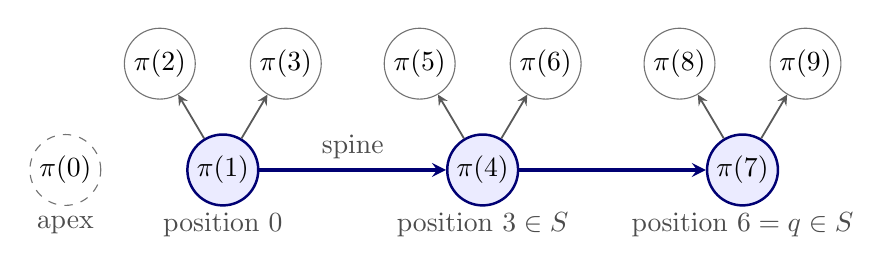
\begin{tikzpicture}[
 x=1cm,y=1cm,>=stealth,
 every node/.style={font=\normalsize},
 vertex/.style={circle,draw=black!55,fill=white,minimum size=9mm,inner sep=1pt},
 spine vertex/.style={vertex,draw=blue!45!black,fill=blue!8,line width=.9pt},
 leaf edge/.style={->,draw=black!65,line width=.65pt},
 spine edge/.style={->,draw=blue!45!black,line width=1.2pt},
 annotation/.style={font=\normalsize,text=black!70}
]
\node[vertex,dashed] (apex) at (-2,0) {$\pi(0)$};
\node[annotation] at (-2,-.7) {apex};

\node[spine vertex] (h0) at (0,0) {$\pi(1)$};
\node[spine vertex] (h3) at (3.3,0) {$\pi(4)$};
\node[spine vertex] (h6) at (6.6,0) {$\pi(7)$};
\node[annotation] at (0,-.7) {position $0$};
\node[annotation] at (3.3,-.7) {position $3\in S$};
\node[annotation] at (6.6,-.7) {position $6=q\in S$};

\node[vertex] (l1) at (-.8,1.35) {$\pi(2)$};
\node[vertex] (l2) at (.8,1.35) {$\pi(3)$};
\node[vertex] (l4) at (2.5,1.35) {$\pi(5)$};
\node[vertex] (l5) at (4.1,1.35) {$\pi(6)$};
\node[vertex] (l7) at (5.8,1.35) {$\pi(8)$};
\node[vertex] (l8) at (7.4,1.35) {$\pi(9)$};

\draw[spine edge] (h0) -- node[above,annotation] {spine} (h3);
\draw[spine edge] (h3) -- (h6);
\draw[leaf edge] (h0) -- (l1);
\draw[leaf edge] (h0) -- (l2);
\draw[leaf edge] (h3) -- (l4);
\draw[leaf edge] (h3) -- (l5);
\draw[leaf edge] (h6) -- (l7);
\draw[leaf edge] (h6) -- (l8);
\end{tikzpicture}
\caption{A labelled caterpillar with $N=10$ and $S=\{3,6\}$. The spine
$\pi(1)\to\pi(4)\to\pi(7)$ has two leaves at each vertex;
all arrows point from parent to child. The apex $\pi(0)$ is separate
from the tree. The last spine position is $q=6$, so the head function
is $h_{\pi,S}(x)=x_{\pi(7)}-x_{\pi(0)}$.}
\label{fig:caterpillar}
\end{figure}

The term \emph{face function} comes from the following geometry.
Identify $a(x)=\langle a,x\rangle$ with its coefficient vector. Then
$\ell_{ij}=e_i-e_j$ points from $e_j$ to $e_i$, and
$h=h_{\pi,S}=e_{\pi(q+1)}-e_{\pi(0)}$ points from the apex label to the
last spine label. Each $\ell\in L=L_{\pi,S}$ points from child to parent.
As free vectors, $h$ places a base corner and the $\ell$ generate its edges.
The polytope apex is $0$, distinct from the labelled point $e_{\pi(0)}$.
Define the \emph{support function} and the caterpillar polytope by
\begin{align}
 h_P(x)&:=\max_{p\in P}\langle p,x\rangle,\label{eq:support-function}\\
 Q_{h,L}&:=\operatorname{conv}\Bigl(\{0\}\cup\Bigl(h+\sum_{\ell\in L}[0,\ell]\Bigr)\Bigr),\qquad
 U_{h,L}=h_{Q_{h,L}}.\label{eq:unit-polytope}
\end{align}
Indeed, the segment $[0,\ell]$ has support function $\relu\circ\ell$, Minkowski sums add support functions, and adjoining $0$ applies the outer ReLU.
The base is the translated zonotope $h+\sum_{\ell\in L}[0,\ell]$.
For a state $\tau$ in~\Cref{eq:faces}, set
$t_\ell=\mathds{1}_{\{\tau(\ell)=\ell\}}$, where $\mathds{1}$ denotes the indicator.
It is zero for omitted edges and hinges; the latter contribute segments.
The corresponding polytope is
$Q^\tau_{h,L}:=\operatorname{conv}\bigl(\{0\}\cup(h+\sum_{\ell\in L}t_\ell\ell+\sum_{\tau(\ell)=\relu\circ\ell}[0,\ell])\bigr)$,
and $U^\tau_{h,L}=h_{Q^\tau_{h,L}}$.
\Cref{fig:polytope-normalization} illustrates the translated generators
for $N=4$ on the slice $x_0=0$, where $a$ becomes $(a_1,a_2,a_3)$ and
$e_0$ is represented by $0$.



The head connects the apex label to the tree, so the head and $N-2$ edge
functions are linearly independent. Thus the base is an $(N-2)$-dimensional
zonotope with affine hull avoiding $0$, and $Q_{h,L}$ is an
$(N-1)$-dimensional pyramid. Each nontrivial face containing $0$ cones over
a base face. Maximizing on each base segment selects $0$, $\ell$, or
$[0,\ell]$, with support functions $0$, $\ell$, and $\relu\circ\ell$;
the outer ReLU adjoins the apex. These are precisely the three states
in~\Cref{eq:faces}.

\Needspace{8\baselineskip}
\begin{definition}[Dictionary, \leandecl{MaxCaterpillar/Construction.lean}{68}{dictionary}]\label{def:dictionary}
The \emph{dictionary} $\D$ is the finite set of functions $\R^N\to\R$ consisting of every face function $U^{\tau}_{\pi,S}$, over all caterpillar descriptions $(\pi,S)$ and all states $\tau$, together with the \emph{auxiliary functions}
\begin{align}\label{eq:aux_functions}
 \begin{aligned}
 &x\mapsto\relu(x_i),\quad x\mapsto\relu(-x_i)
 &&(0\leq i<N),\\
 &x\mapsto\relu(x_i-x_j)
 &&(0\leq i<j<N).
 \end{aligned}
\end{align}
\end{definition}
Heads and edge functions are coordinate differences, so face functions and the functions $x\mapsto\relu(x_i-x_j)$ are translation invariant: with $\one:=(1,\ldots,1)\in\R^N$,
\begin{align}\label{eq:translation-invariance}
 U^{\tau}_{\pi,S}(x+t\one)=U^{\tau}_{\pi,S}(x)\qquad(t\in\R).
\end{align}
Only $\relu(\pm x_i)$ change under this translation.
\Cref{thm:dictionary} proves that $\D$ spans the maximum.
\Cref{sec:compression} chooses rational coefficients from one basis of its
span, without integration.

\subsection{The network}\label{sec:network}

The network computes an expansion of $\maxn_N$ in face functions and
auxiliary functions. To compile face functions, first absorb every linear edge of a face state into the head:
\begin{align}\label{eq:face-description}
 U^{\tau}_{h,L}=U_{h',M},\qquad
 h':=h+\sum_{\tau(\ell)=\ell}\ell,\qquad
 M:=\{\ell\in L:\tau(\ell)=\relu\circ\ell\}.
\end{align}
By~\Cref{eq:hinge-reversal}, reversing each remaining $\ell_{ij}$ with
$i>j$ gives the same function with the \emph{normalized description}
\begin{align}\label{eq:normalized-description}
\begin{aligned}
   M^+&:=\{\ell_{\min(i,j),\max(i,j)}:\ell_{ij}\in M\},\\
   h^+&:=h'+\sum_{\ell_{ij}\in M,\ i>j}\ell_{ij}.
\end{aligned}
\end{align}
Geometrically, $[0,\ell]=\ell+[0,-\ell]$: reversing a generator shifts the
head by the old generator. Normalization chooses a consistent orientation
and a corresponding base corner; it does not rescale vectors or change the
polytope (\Cref{fig:polytope-normalization}).
Write $U_k:=U_{h,M}$ for a normalized description $k=(h,M)$, and let
$\mathcal K_0$ be the set of normalized descriptions of all face functions.
Let $A_N$ be the span of the auxiliary functions~\Cref{eq:aux_functions}.
The network has three parts (\Cref{fig:architecture}).
\begin{itemize}
\item The \emph{first hidden layer} computes the shared features
\begin{align}\label{eq:features}
\Phi(x):=\bigl(\relu(x_0),\ \relu(-x_0),\ (\relu(x_i-x_0))_{i>0},\ (\relu(x_i-x_j))_{i<j}\bigr).
\end{align}
\item The \emph{second hidden layer} computes the retained units $U_k$,
$k\in K$, for a set $K\subseteq\mathcal K_0$, and the two neurons
$\relu(R)$ and $\relu(-R)$ for an auxiliary remainder $R\in A_N$.
\item The \emph{output layer} returns
$\sum_{k\in K}d_kU_k+\relu(R)-\relu(-R)$.
\end{itemize}

\begin{figure}[htbp]
\centering
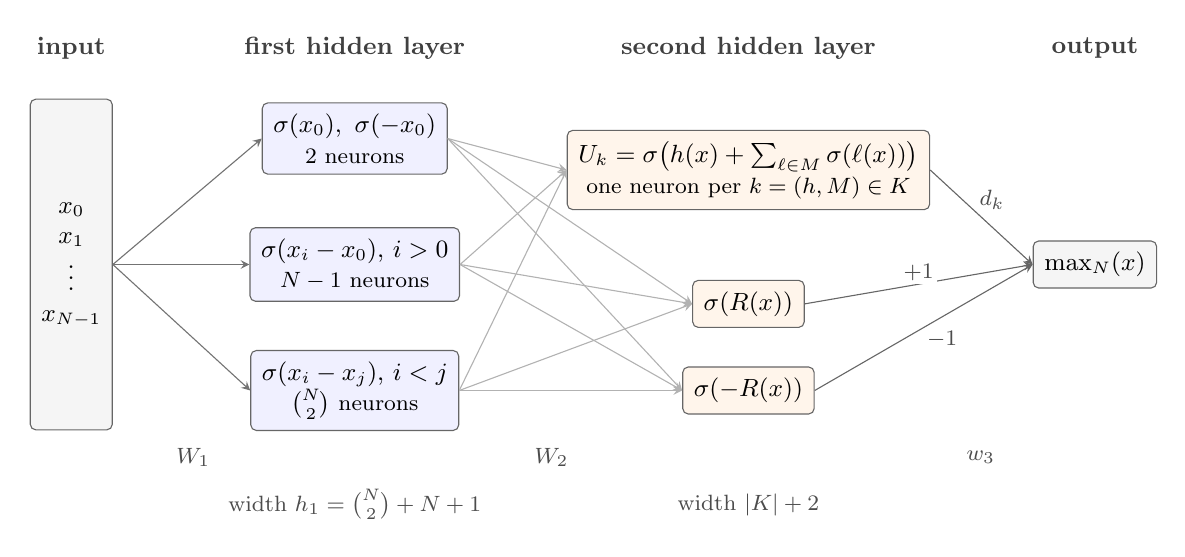
\begin{tikzpicture}[x=1cm,y=1cm,>=stealth,
 box/.style={draw=black!60,rounded corners=2pt,fill=#1,inner sep=4pt,align=center,font=\small},
 head/.style={font=\small\bfseries,text=black!75},
 wt/.style={font=\footnotesize,text=black!70,fill=white,inner sep=1pt}]
\node[head] at (0,2.75) {input};
\node[head] at (3.6,2.75) {first hidden layer};
\node[head] at (8.6,2.75) {second hidden layer};
\node[head] at (13,2.75) {output};
\node[box=black!4,minimum height=4.2cm] (in) at (0,0) {$x_0$\\$x_1$\\$\vdots$\\$x_{N-1}$};
\node[box=blue!6] (f1) at (3.6,1.6) {$\relu(x_0),\ \relu(-x_0)$\\{\footnotesize $2$ neurons}};
\node[box=blue!6] (f2) at (3.6,0) {$\relu(x_i-x_0)$, $i>0$\\{\footnotesize $N-1$ neurons}};
\node[box=blue!6] (f3) at (3.6,-1.6) {$\relu(x_i-x_j)$, $i<j$\\{\footnotesize $\binom N2$ neurons}};
\node[box=orange!8] (u) at (8.6,1.2) {$U_k=\relu\bigl(h(x)+\sum_{\ell\in M}\relu(\ell(x))\bigr)$\\{\footnotesize one neuron per $k=(h,M)\in K$}};
\node[box=orange!8] (rp) at (8.6,-0.5) {$\relu(R(x))$};
\node[box=orange!8] (rm) at (8.6,-1.6) {$\relu(-R(x))$};
\node[box=black!4] (out) at (13,0) {$\maxn_N(x)$};
\foreach \f in {f1,f2,f3} \draw[->,black!55] (in.east) -- (\f.west);
\foreach \f in {f1,f2,f3} \foreach \g in {u,rp,rm} \draw[->,black!30] (\f.east) -- (\g.west);
\draw[->,black!60] (u.east) -- node[wt,pos=0.45,above right] {$d_k$} (out.west);
\draw[->,black!60] (rp.east) -- node[wt,pos=0.5,above] {$+1$} (out.west);
\draw[->,black!60] (rm.east) -- node[wt,pos=0.5,below right] {$-1$} (out.west);
\node[wt] at (1.55,-2.45) {$W_1$};
\node[wt] at (6.1,-2.45) {$W_2$};
\node[wt] at (11.55,-2.45) {$w_3$};
\node[font=\footnotesize,text=black!70] at (3.6,-3.05) {width $h_1=\binom N2+N+1$};
\node[font=\footnotesize,text=black!70] at (8.6,-3.05) {width $|K|+2$};
\end{tikzpicture}
\caption{The Caterpillar Net. The first hidden layer is fixed. The second
hidden layer has one neuron for every retained normalized description
$k=(h,M)$ and two neurons for the auxiliary remainder $R$. All biases are
zero; the matrices are given in~\Cref{eq:network-assembly}.}
\label{fig:architecture}
\end{figure}

\Needspace{8\baselineskip}
\begin{theorem}[Compilation, \leandecl{MaxCaterpillar/Core.lean}{30}{compilation}, {\Cref{pf:thm:compilation}}]\label{thm:compilation}
Let $K\subseteq\mathcal K_0$, $d\in\R^K$, and $R\in A_N$ satisfy
\begin{align}\label{eq:compilation-hypothesis}
 \maxn_N=\sum_{k\in K}d_kU_k+R.
\end{align}
Then the network with first hidden layer~\Cref{eq:features} and the matrices
in~\Cref{eq:network-assembly} computes $\maxn_N$. It has widths $h_1$ and
$|K|+2$ and zero biases. Its weights are rational whenever the coefficients
$d_k$ and the auxiliary coefficients of $R$ are rational.
\end{theorem}

\begin{Proof}{Theorem}{thm:compilation}
The first hidden layer outputs $\Phi$ from~\Cref{eq:features}.
Thus $W_1$ has rows $e_0^\top$ and $-e_0^\top$, then $e_i^\top-e_0^\top$ for $i>0$, then $e_i^\top-e_j^\top$ for $i<j$, using a fixed ordering within each block. Its row count is
\begin{align}\label{eq:feature-count}
\binom N2+(N-1)+2=\binom N2+N+1=h_1.
\end{align}
By~\Cref{eq:hinge-reversal}, these features recover all coordinates,
\begin{align}\label{eq:recover-coordinates}
\begin{aligned}
x_0&=\relu(x_0)-\relu(-x_0),\\
x_i&=x_0+\relu(x_i-x_0)-\relu(x_0-x_i)\qquad(i>0).
\end{aligned}
\end{align}
For each $k=(h,M)\in K$, substitute~\Cref{eq:recover-coordinates} into $h(x)+\sum_{\ell\in M}\relu(\ell(x))$ and collect the coefficients of $\Phi(x)$ into a row vector $w_k^\top$. Every hinge in $M$ already has the orientation $i<j$, so its coefficient is added directly to the corresponding feature.

To specify the remaining row, collect the auxiliary coefficients of $R$ as
\begin{align}\label{eq:auxiliary-remainder}
R(x)=\sum_i p_i\relu(x_i)+\sum_i n_i\relu(-x_i)+\sum_{i<j}s_{ij}\relu(x_i-x_j).
\end{align}
Each retained unit is translation invariant by~\Cref{eq:translation-invariance}, and $\maxn_N(x+t\one)=\maxn_N(x)+t$, so~\Cref{eq:compilation-hypothesis} gives
\begin{align}\label{eq:remainder-translation}
R(x+t\one)=R(x)+t,\qquad \sum_i p_i=1.
\end{align}
The coefficient sum follows by setting $x=0$ and $t=1$. Now choose $t$ large enough that every $x_i+t$ is nonnegative. Substituting the auxiliary expansion into~\Cref{eq:remainder-translation} cancels $t$ and gives
\begin{align}\label{eq:compact-remainder}
R(x)=\sum_i p_ix_i+\sum_{i<j}s_{ij}\relu(x_i-x_j).
\end{align}
Substitute~\Cref{eq:recover-coordinates} into this expression and collect the coefficients of $\Phi(x)$ into $w_R$. Thus both $w_k$ and $w_R$ are specified by finite sums of the previously defined coefficients. The entries of $W_1$ and of the rows $w_k$ are integers, because heads and hinges are integer combinations of coordinates. The row $w_R$ is a rational combination of the $p_i$ and $s_{ij}$, and $w_3$ consists of the $d_k$ and $\pm1$.

Order $K$ and set the second hidden layer matrix and output layer vector to
\begin{align}\label{eq:network-assembly}
W_2=\begin{pmatrix}(w_k^\top)_{k\in K}\\w_R^\top\\-w_R^\top\end{pmatrix},\qquad
w_3=\begin{pmatrix}(d_k)_{k\in K}\\1\\-1\end{pmatrix},\qquad b_1=b_2=b_3=0.
\end{align}
The second hidden layer outputs $U_k(x)$ and $\relu(\pm R(x))$. By~\Cref{eq:hinge-reversal} and~\Cref{eq:compilation-hypothesis},
\begin{align}\label{eq:signed-remainder}
w_3^\top\relu(W_2\Phi(x))=\sum_{k\in K}d_kU_k(x)+\relu(R(x))-\relu(-R(x))=\maxn_N(x).
\end{align}
\end{Proof}

\Cref{thm:quotient-compression} gives such an expansion with rational
coefficients; \Cref{sec:size} counts the normalized descriptions that can
occur.

\section{Lower bounds for caterpillar expansions}\label{sec:lower}

The second width of the network of \Cref{thm:compilation} is the number of
caterpillar functions in an expansion of $\maxn_N$, plus two. This section
shows that this number must grow exponentially, and that the vocabulary
itself is large.

\Needspace{6\baselineskip}
\begin{definition}[Caterpillar expansion, \leandecl{MaxCaterpillar/Definitions.lean}{98}{IsCaterpillarExpansion}]\label{def:caterpillar-expansion}
A finite set $K\subseteq\mathcal K_0$ is a \emph{caterpillar expansion} of
$\maxn_N$ if there are real numbers $d_k$, $k\in K$, and a function $R\in A_N$
with $\maxn_N=\sum_{k\in K}d_kU_k+R$ on $\R^N$. Its \emph{size} is $|K|$.
\end{definition}

\Needspace{10\baselineskip}
\begin{theorem}[Exponential count, \leandecl{MaxCaterpillar/Theorems.lean}{113}{caterpillar_expansion_choose_le}, \leandecl{MaxCaterpillar/Theorems.lean}{121}{caterpillar_expansion_exponential}, \leandecl{MaxCaterpillar/Theorems.lean}{155}{caterpillar_expansion_quadratic}, {\Cref{pf:thm:count-exponential}}]\label{thm:count-exponential}
Let $N\geq3$ and let $K$ be a caterpillar expansion of $\maxn_N$. Then
\begin{align}
 \binom Nm&\leq6^m\,|K|\qquad(3\leq m\leq N),\label{eq:count-binomial}\\
 7^N&\leq(N+1)\,6^N\,|K|,\label{eq:count-exponential}\\
 N(N-1)&\leq6\,|K|.\label{eq:count-quadratic}
\end{align}
In particular $|K|\geq(7/6)^N/(N+1)$, and every network of the form of
\Cref{thm:compilation} for $\maxn_N$ has second width at least
$(7/6)^N/(N+1)+2$.
\end{theorem}

The bound~\Cref{eq:count-exponential} follows from~\Cref{eq:count-binomial}
by summing over all $m$ with the binomial theorem; it exceeds
the quadratic bound~\Cref{eq:count-quadratic} only for $N$ of order $70$.
The idea of the proof (\Cref{app:lower}) is local. At a point where
$m\geq3$ coordinates tie at the top and the others lie strictly below in a
fixed order, the $m$-th mixed difference in the tied coordinates annihilates
every auxiliary function, which depends on at most two coordinates, and does
not annihilate $\maxn_N$. Hence some $U_k$ with $k\in K$ is nonlinear in all
tied coordinates there. The caterpillar structure allows a single $U_k$ to
do so only at a fraction $6^m/\binom Nm$ of these points.

The same bound applies to a larger vocabulary. For an integer head $h$ and
a set $M$ of oriented edges of a forest, write
$U(x)=\relu(\sum_i h_ix_i+\sum_{(i,j)\in M}\relu(x_i-x_j))$ and
$\kappa_i=h_i+|\{j:(i,j)\in M\}|$.
Delete, simultaneously, all degree-one vertices with $\kappa_i=0$ from
the forest; call the result its \emph{reduced forest}.

\begin{theorem}[Forest expansions, \leandecl{MaxCaterpillar/Count/Main.lean}{26}{choose_le_of_unit_bound}, {\Cref{pf:thm:forest-count}}]\label{thm:forest-count}
Let $\Delta\geq2$ be an integer. Suppose
$\maxn_N=\sum_{k\in K}d_kU_k+R$, where $R\in A_N$ and every $U_k$ has an
integer head and a forest of functions $\relu(x_i-x_j)$ whose reduced
forest has maximum degree at most $\Delta$. Put $b=2\Delta+2$. Then
\begin{align}\label{eq:forest-count}
 \binom Nm\leq b^m|K|\qquad(3\leq m\leq N).
\end{align}
Consequently $|K|\geq(1+1/b)^N/(N+1)$ for $N\geq3b+2$.
For $\Delta=2$, the latter bound holds for every $N\geq3$.
\end{theorem}

Caterpillar functions have reduced degree at most $2$: their retained leaf
edges have $\kappa_i=0$ at the leaf, and their remaining edges lie on a path.
The rooted stars
$\relu(x_c-x_a+\sum_{l\ne a,c}\relu(x_c-x_l))$
and all their face functions have reduced degree $0$.
Thus the bound $(7/6)^N/(N+1)$ counts all functions in any mixture of these
families, including the building blocks of the direct combinatorial
construction of Brunck et al.\ \cite{BSY}; see \Cref{app:bsy}.
More generally, \Cref{thm:forest-count} covers every tree of bounded degree,
with arbitrary edge orientations, and permits unboundedly many deleted
leaves at each vertex.

\begin{theorem}[Paths and cycles with arbitrary weights, {\Cref{pf:thm:degree-two-weighted}}]\label{thm:degree-two-weighted}
Suppose $N\geq3$ and $\maxn_N=R+\sum_{k\in K}d_kU_k$, where $R$ is a
linear function plus a finite linear combination of ReLUs of linear forms,
and
\begin{align}\label{eq:degree-two-unit}
 U_k(x)=\relu\!\left(h_k(x)+
       \sum_{(i,j)\in M_k}c_{k,ij}\relu(x_i-x_j)\right).
\end{align}
The heads $h_k$ are arbitrary linear functions, all coefficients are arbitrary
real numbers, and each $M_k$ orients a simple graph of maximum degree at most
two. Then
\begin{align}\label{eq:degree-two-count}
 \binom Nm\leq\left(N+\frac{m-1}{2}N^2\right)|K|
 \qquad(3\leq m\leq N).
\end{align}
Taking $m=\lfloor N/2\rfloor$ gives
$|K|=\Omega(2^N/N^{7/2})$ as $N\to\infty$.
The conclusion remains valid when biases are allowed.
\end{theorem}

The comparison graphs in \Cref{thm:degree-two-weighted} may be disconnected
unions of paths and cycles. The same locality argument extends to
\emph{pseudoforests}: graphs with at most one cycle in each connected component.

\begin{theorem}[Weighted comparison graphs, {\Cref{pf:thm:weighted-forest}}]\label{thm:weighted-forest}
Let $N\geq3$. Use the representation and coefficient assumptions of
\Cref{thm:degree-two-weighted}, with comparison pseudoforests $G_j$.
Write $\nu(G_j)$ for their maximum matching sizes and $z(G_j)$ for their
numbers of isolated vertices. If $\nu(G_j)+z(G_j)\geq k$ for a nonnegative
integer $k$ and every $j$, put
$b_N=1+N+\binom N2$ and $c_k=1+k/3+\binom k2/9$. Then
\begin{align}\label{eq:weighted-forest-count}
 |K|\geq\frac{1-b_N2^{-N}}{c_k}\left(\frac43\right)^k.
\end{align}
If the maximum degrees are at most $\Delta$, one may take
$k=\lceil N/(\Delta+1)\rceil$, giving
$|K|=\Omega_\Delta((4/3)^{N/(\Delta+1)}/N^2)$.
For arbitrary comparison graphs of maximum degree at most $\Delta\geq1$, put
$q_\Delta=\Delta^\Delta/(\Delta+1)^{\Delta+1}$. The corresponding bound is
$\Omega_\Delta((1-q_\Delta)^{-N/(\Delta+1)}/N^{2/(\Delta+1)})$.
These bounds also hold for the number of distinct comparison graphs used.
\end{theorem}

Degree in these two theorems refers to the full graph, before any leaf
deletion. Every fixed $\Delta$ therefore gives an exponential lower bound,
with arbitrary orientations, heads, weights, and biases. The proofs use the
rank of the comparisons at a tied maximum and elementary counting; they are
not yet formalized in Lean. A matching of linear size in each pseudoforest
also gives an exponential bound without restricting the maximum degree.
Trees of unbounded degree and
sublinear matching number remain outside this exponential regime.

Additional cycles are allowed. Put
$b(G)=\sum_C\max\{0,|E(C)|-|V(C)|\}$ for a comparison graph $G$, summing over
its connected components.
If every graph has $\nu(G)+z(G)\geq k$ and $b(G)\leq b$, then
\begin{align}\label{eq:bounded-excess-count}
 |K|\geq\frac{1-b_N2^{-N}}
 {\Pr\bigl(\operatorname{Bin}(k,1/4)\leq b+2\bigr)}.
\end{align}
Thus a matching of linear size and $b=o(N)$ still give an exponential
bound, without any degree restriction. More generally it suffices that
$k=\Omega(N)$ and $\limsup b/k<1/4$. The proof is in
\Cref{app:count-exponential}.

\paragraph[Trees with few out-leaves]{Trees with few out-leaves (\leandecl{MaxCaterpillar/Count/Main.lean}{228}{outLeaf_unified_exponential}).}
There is also an exponential bound without restricting internal branching.
In the normalized description of a tree face function, call a vertex an
\emph{out-leaf} if it has degree one in the retained forest and $\kappa_i=1$.
If every vertex of every tree function is adjacent to at most $s\geq1$
out-leaves, then any expansion by these functions together with caterpillar
functions satisfies
$|K|\geq(1+1/(2s+4))^N/(N+1)$ for $N\geq3$,
where $K$ counts both families.
Thus the relevant restriction concerns the oriented edges and head of each
function, rather than just the shape of its original tree.

For example, take \emph{any} tree $T$ on the labels other than an apex $a$,
choose vertices $s,r$ of $T$, orient every edge away from $s$, and retain
all the functions $\relu(x_p-x_q)$ on those oriented edges. The resulting
function is
$U_{a,s,r,T}(x)=\relu(x_r-x_a+
       \sum_{p\to q\text{ in }T}\relu(x_p-x_q))$.
At a tree vertex $v$, normalization gives
$\kappa_v=\deg_T(v)-1+\mathbf1_{v=s}+\mathbf1_{v=r}$.
Only $s$ and $r$ can therefore be out-leaves. A degree-two covering forest
improves the bound in this case to $(7/6)^N/(N+1)$, even when these functions
are added to the caterpillar and rooted-star face dictionaries; the argument
is given at the end of \Cref{app:count-exponential}.
This includes every underlying tree shape.
It does not include arbitrary face functions of those added trees:
replacing edges by linear terms can create many out-leaves at one vertex.

\paragraph{Large matchings with arbitrary heads and weights.}
The matching argument also works in mixtures containing the original
constructions. Let $N\geq3$ and $0\leq2k\leq N$.
Adjoin to the caterpillar and rooted-star face dictionaries all functions of
the form \Cref{eq:degree-two-unit} whose comparison pseudoforest on the $N$ labels
has a matching of size at least $k$. The heads and all coefficients may be
arbitrary real numbers. Every expansion of $\maxn_N$ in this enlarged dictionary,
with an auxiliary remainder, uses at least
$(169/147)^k/(N+1)^2$ functions. The proof at the end of
\Cref{app:count-exponential} is mathematical; this extension is not yet
formalized in Lean.

In particular, every canonical tree orientation and face state is covered when
$k\geq\varepsilon(N-1)$ for a fixed $\varepsilon>0$. This includes all trees
with a perfect or near-perfect matching, and every star whose edges are
subdivided once. More generally, a tree on $n\geq2$ vertices with $L$ leaves
has a matching of size at least $(n-L+1)/2$, so a fixed positive fraction of
nonleaf vertices suffices. The enlarged dictionary still spans the maximum
because it contains the original caterpillar dictionary.

\paragraph{Stars with arbitrary orientations.}
All star face functions can also be adjoined, with arbitrary head roots,
edge orientations, and face states. The caterpillar dictionary together
with this entire star family still requires at least
$(7/6)^N/(N+1)^4$ nonstar terms for $N\geq5$.
If the matching class above is included as well, the corresponding bound
is $(169/147)^k/(N+1)^4$ on the terms outside the added star family.
This follows by propagating an exactly checked five-label separator through
coordinate deletions; the argument is given in \Cref{app:count-exponential}.
It is not yet a Lean result. Nonstar trees with sublinear matching number
remain unresolved in general, so the unrestricted all-tree exponential
bound is still open.

\Needspace{6\baselineskip}
\begin{theorem}[Vocabulary dimension, \leandecl{MaxCaterpillar/Theorems.lean}{192}{caterpillarDim_ge}, {\Cref{pf:thm:quotient-lower}}]\label{thm:quotient-lower}
For every $N\geq3$, the span $V_N:=\spn\D$ of the dictionary satisfies
$q_N:=\dim(V_N/A_N)\geq(N-2)!$.
\end{theorem}

Thus \Cref{thm:quotient-compression} cannot give a second width below
$(N-2)!+2$; together with \Cref{thm:main}, $\log q_N=\Theta(N\log N)$.
These bounds concern the stated dictionaries; they do not give a width
lower bound for general two-hidden-layer networks.

% Begin sections/dictionary.tex
\section{Why the dictionary spans the maximum}\label{sec:dictionary}

The maximum is the support function of a simplex. To work in its affine dimension, set
\begin{align}\label{eq:simplex}
 \Delta:=\operatorname{conv}\{0,e_1,\ldots,e_{N-1}\}\subseteq H_0:=\{x\in\R^N:x_0=0\}.
\end{align}
For every $x\in\R^N$,
\begin{align}\label{eq:full-coordinates}
 \maxn_N(x)=x_0+h_\Delta(x-x_0\one).
\end{align}
It suffices to prove that $h_\Delta$ lies in the span of the restrictions of
$\D$ to $H_0$: the substitution $x\mapsto x-x_0\one$ fixes every face
function, sends coordinate features to $\relu(\pm(x_i-x_0))$, and preserves
the dictionary span by~\Cref{eq:hinge-reversal}.

Henceforth all polytopes lie in $H_0$, and heads and edge functions are
identified with their restricted coefficient vectors. Let $\LS_k$ be the
real span of support functions of polytopes of affine dimension at most
$k$; thus $\LS_0$ consists of linear functions. The \emph{exposed face}
of $P$ in direction $u\in H_0$ is
\begin{align}\label{eq:exposed-face}
 P^u:=\{p\in P:\langle p,u\rangle=h_P(u)\}.
\end{align}
The opposite face $P^{-u}$ consists of the minimizers. Define
\begin{align}\label{eq:facet-difference}
 D_uh_P(x):=h_{P^u}(x)-h_{P^{-u}}(x)
 \qquad(x\in H_0).
\end{align}
Here $u$ selects the faces, while $x$ is the support-function input;
$P^0=P$ gives $D_0=0$. For a simplex facet normal, $D_u$ subtracts the
opposite vertex's linear support function from that of the facet.

\Needspace{6\baselineskip}
For a finite linear combination $g$ of support functions, define its one-sided directional derivative at $u$ by
\begin{align}\label{eq:face-derivative}
\begin{aligned}
\partial_u g(x)&:=\lim_{t\downarrow0}\frac{g(u+tx)-g(u)}{t},\\
\partial_u h_P&=h_{P^u},\qquad D_ug=\partial_ug-\partial_{-u}g.
\end{aligned}
\end{align}
This makes $D_u$ independent of the support-function decomposition. When
$\langle u,\cdot\rangle$ is constant on $P$, the exposed faces cancel;
otherwise both have smaller dimension. Consequently,
\begin{align}\label{eq:face-dimension-drop}
D_u\LS_k\subseteq\LS_{k-1}\qquad(k\geq1).
\end{align}

\paragraph{The signed caterpillar sum.}
We seek a combination that agrees with $h_\Delta$ up to a function in $\LS_{N-2}$.
Adding $x_{\pi(0)}$ makes the caterpillar function the following maximum
\begin{align}\label{eq:apex-maximum}
  x_{\pi(0)}+U_{\pi,S}(x)=\max\left\{x_{\pi(0)},\,x_{\pi(q+1)}+\sum_{\ell\in L_{\pi,S}}\sigma(\ell(x))\right\}.
\end{align}
Averaging over permutations gives
the required symmetry
\begin{align}\label{eq:signed-word-sum}
 F_N(x):=\frac{1}{N!}\sum_{\pi}
   \sum_{\varnothing\ne S\subseteq\{1,\ldots,r\}}
   (-1)^{N+|S|}\bigl(x_{\pi(0)}+U_{\pi,S}(x)\bigr),
\end{align}
The signs cancel the extra exposed-face contributions modulo $\LS_{N-3}$,
as proved below.

\Needspace{8\baselineskip}
\begin{theorem}[Dictionary sufficiency, \leandecl{MaxCaterpillar/Lemmas.lean}{54}{maximum_mem_dictionary}, {\Cref{pf:thm:dictionary}}]\label{thm:dictionary}
For every $N\geq3$, the dictionary of \Cref{def:dictionary}
satisfies
\begin{align}\label{eq:dictionary-span}
 \maxn_N\in\spn\D.
\end{align}
\end{theorem}

\begin{Proof}{Theorem}{thm:dictionary}
Define the error by
\begin{align}\label{eq:facet-error}
f:=F_N|_{H_0}-h_\Delta.
\end{align}
\Cref{stp:corrections} reduces dictionary membership to $f\in\LS_{N-2}$;
\Cref{stp:reconstruction} reduces this to $D_uf\in\LS_{N-3}$ for all $u$.
\Cref{stp:class} proves these bounds by cancellation, using induction only
when deleting a single exceptional coordinate.

\pfstep{stp:corrections}{Reduce to a lower-dimensional error}
Assume temporarily that
\begin{align}\label{eq:class-identity}
  f=F_N-h_\Delta\in\LS_{N-2}.
\end{align}
Write $Q_{\pi,S}:=Q_{h_{\pi,S},L_{\pi,S}}$. Removing the linear apex terms
from~\Cref{eq:signed-word-sum} gives
\begin{align}\label{eq:geometric-class}
\frac{1}{N!}\sum_{\pi}\sum_{\varnothing\ne S\subseteq\{1,\ldots,N-2\}}(-1)^{N+|S|}h_{Q_{\pi,S}}-h_\Delta\in\LS_{N-2}.
\end{align}

We correct the error by subtracting derivatives $\partial_u$ until it is
linear. Faces of $Q_{\pi,S}$ already have support functions in the dictionary
span: apex--base faces give~\Cref{eq:faces}, base faces give linear
functions plus hinges, and the apex alone gives zero. Coordinate features
and~\Cref{eq:hinge-reversal} represent the linear terms and either hinge
orientation. Differentiating $h_\Delta$ also produces simplex faces;
induction on their vertex count supplies these functions.

\pfclaim{clm:simplex-faces}{Simplex faces, \leandecl{MaxNN/Constructions/Paramid/Geom/Faces/ConeOnly.lean}{40}{hS_mem_of_subset_simplexVerts}, \leandecl{MaxNN/Constructions/Paramid/Geom/Faces/ConeOnly.lean}{71}{simplex_sub_mem_coneFaceSpan}, {\Cref{pf:clm:simplex-faces}}}
For every nonempty $T\subseteq\{0,e_1,\ldots,e_{N-1}\}$, the support function of $\Delta_T:=\operatorname{conv}T$ lies in the dictionary span.

\phantomsection\label[proof]{pf:clm:simplex-faces}
\paragraph{Start ($|T|=1$).}
The support function of a singleton is linear and lies in the dictionary span.

\paragraph{Step ($|T|\geq2$).}
Fix $T$ and assume the claim for all smaller nonempty vertex sets. For any
current vertex set $A$ with $|A|\geq2$, remove $v\in A$ using a direction
whose value at $v$ exceeds its common value at the other vertices. Writing
$\Delta_A:=\operatorname{conv}A$, this gives
\begin{align}\label{eq:simplex-vertex-removal}
\begin{aligned}
u_v&:=\begin{cases}-\sum_{i=1}^{N-1}e_i&v=0,\\v&v\ne0,\end{cases}\\
(\Delta_A)^{u_v}&=\{v\},\qquad (\Delta_A)^{-u_v}=\Delta_{A\setminus\{v\}},\\
D_{u_v}h_{\Delta_A}(x)&=\langle v,x\rangle-h_{\Delta_{A\setminus\{v\}}}(x).
\end{aligned}
\end{align}
Order the vertices outside $T$ as $v_1,\ldots,v_{N-|T|}$ and set
\begin{align}\label{eq:initial-simplex-error}
\varepsilon_T:=D_{u_{v_{N-|T|}}}\cdots D_{u_{v_1}}\left(\frac{1}{N!}\sum_\pi\sum_{\varnothing\ne S\subseteq\{1,\ldots,N-2\}}(-1)^{N+|S|}h_{Q_{\pi,S}}-h_\Delta\right).
\end{align}
Each deletion changes the sign of the remaining simplex term, and subsequent $D_u$ annihilate the linear terms. Hence
\begin{align}\label{eq:simplex-deletion-sign}
D_{u_{v_{N-|T|}}}\cdots D_{u_{v_1}}h_\Delta=(-1)^{N-|T|}h_{\Delta_T}+\ell_T,
\end{align}
where $\ell_T$ is linear. Thus the coefficient of $h_{\Delta_T}$ in
$\varepsilon_T$ is $(-1)^{N-|T|+1}$; all other terms are linear or
caterpillar-face support functions and lie in $\spn\D$.
By~\Cref{eq:face-dimension-drop}, $\varepsilon_T\in\LS_{|T|-2}$.
For the full vertex set the empty composition is the identity.

Lower the residual dimension recursively by
\begin{align}\label{eq:error-peeling}
\begin{aligned}
\varepsilon_T^{(0)}(x)&:=\varepsilon_T(x),\\
\varepsilon_T^{(j+1)}(x)&:=\varepsilon_T^{(j)}(x)-\sum_{u\in E_{T,j}}\bigl(\partial_u\varepsilon_T^{(j)}\bigr)(x).
\end{aligned}
\end{align}
Here $0\leq j<|T|-2$; the next claim chooses each finite $E_{T,j}\subseteq H_0$.

\pfclaim{clm:residual-reduction}{Residual reduction, \leandecl{MaxNN/Constructions/Paramid/Geom/Faces.lean}{69}{mem_GSpanRel_sup_of_lt_finrank}, {\Cref{pf:clm:residual-reduction}}}
The sets $E_{T,j}$ can be chosen successively so that, for $0\leq j\leq|T|-2$,
\begin{align}\label{eq:residual-invariant}
\begin{aligned}
\varepsilon_T^{(j)}&\in\LS_{|T|-2-j},\\
\varepsilon_T-\varepsilon_T^{(j)}&\in\spn\D.
\end{aligned}
\end{align}
Each residual remains a linear combination of $h_{\Delta_T}$, support
functions of its proper faces and of caterpillar faces, and linear functions.

\noindent The proof in \Cref{app:residual} chooses a direction orthogonal
to each maximal-dimensional direction space, avoiding orthogonality to
the simplex and other spaces. The derivative sum preserves each maximal
term exactly once; subtracting it lowers the dimension.

At stage $j=|T|-2$, the error is linear, so~\Cref{eq:residual-invariant}
gives $\varepsilon_T\in\spn\D$. Its simplex coefficient is $\pm1$, and its
other terms already lie in the span; hence $h_{\Delta_T}\in\spn\D$.
Taking the full vertex set proves $h_\Delta\in\spn\D$ under
assumption~\Cref{eq:class-identity}.

\pfstep{stp:reconstruction}{Why the facet bounds imply the class identity}
For $N\geq4$ and $f=F_N-h_\Delta$, we show that $f\in\LS_{N-2}$ follows from
\begin{align}\label{eq:facet-reduction}
D_uf\in\LS_{N-3}\qquad\text{for every }u\in H_0.
\end{align}
The base zonotope admits the Freudenthal--Kuhn triangulation
\cite{Freudenthal1942,Kuhn1960}; coning it to the apex expresses each
caterpillar support function as a sum of simplex support functions modulo
$\LS_{N-2}$. For a simplex, $D_u$ isolates a facet up to the linear support
function of its opposite vertex. Thus~\Cref{eq:facet-reduction} controls
the weighted sums of parallel facets. A common linear reconstruction
operator turns these facet cancellations back into a cancellation of the
original simplex sum. Define
\begin{align}\label{eq:sweep-operation}
(\mathcal Tg)(x):=\begin{cases}g(x)&x_1\geq0,\\g(x-x_1e_1)&x_1<0.\end{cases}
\end{align}

\pfclaim{clm:simplex-reconstruction}{Simplex reconstruction, \leandecl{MaxNN/Constructions/Paramid/Geom/Reconstruct.lean}{83}{simplex_reconstruct_any_height}, {\Cref{pf:clm:simplex-reconstruction}}}
Every $(N-1)$-dimensional simplex $P\subseteq H_0$ satisfies
\begin{align}\label{eq:simplex-reconstruction}
h_P-\mathcal T\left(\sum_{F\text{ facet of }P}\operatorname{sgn}\langle\nu_F,e_1\rangle\,h_F\right)\in\LS_{N-2}.
\end{align}
Here $\nu_F$ is an outward normal of $F$. Its sign against $e_1$ records whether the facet bounds lines parallel to $e_1$ from above or below; parallel facets contribute zero. 
The operator $\mathcal T$ fills the segments between a polytope and its
projection onto $p_1=0$, up to a segment correction for translation; hence
$\mathcal T\LS_k\subseteq\LS_{k+1}$. Applying the claim with the same
operator to every simplex preserves the cancellations between parallel facets. Their sums lie in $\LS_{N-3}$, so their reconstructions lie in
$\LS_{N-2}$, as required. \Cref{app:reconstruction} proves the claim
and the subdivision and grouping steps.

\Needspace{5\baselineskip}
\pfclaim{clm:class-identity}{Class identity, \leandecl{MaxCaterpillar/Lemmas.lean}{48}{class_identity}, {\Cref{pf:clm:class-identity}}}
The class identity~\Cref{eq:class-identity} holds for every $N\geq3$.

\pfstep{stp:class}{Prove the class identity by induction}
\phantomsection\label[proof]{pf:clm:class-identity}
\paragraph{Start ($N=3$).}
Here $S=\{1\}$, $q=1$, and $p(1)=0$, so~\Cref{eq:apex-maximum} gives
\begin{align}\label{eq:base-unit}
\begin{aligned}
x_{\pi(0)}+U_{\pi,\{1\}}(x)&=\max\bigl\{x_{\pi(0)},x_{\pi(2)}+\relu(x_{\pi(1)}-x_{\pi(2)})\bigr\}\\
&=\max\{x_{\pi(0)},x_{\pi(1)},x_{\pi(2)}\}=\maxn_3(x).
\end{aligned}
\end{align}
All six terms have coefficient $1/6$, so
\begin{align}\label{eq:base-formula}
F_3=\maxn_3.
\end{align}
On $H_0$, this gives $f=0\in\LS_1$.

\paragraph{Step ($N\geq4$).}
Assume the class identity for $N-1$. By \Cref{stp:reconstruction}, it
suffices to prove $D_uf\in\LS_{N-3}$ for every $u\in H_0$. The linear apex
terms disappear. The exposed simplex faces have the largest and smallest
coordinate values $u_i$, including $u_0=0$. In a caterpillar base,
$[0,\ell_{ij}]$ remains free when $u_i=u_j$; its maximizing endpoint is
$\ell_{ij}$ when $u_i>u_j$ and $0$ when $u_i<u_j$. Minimization reverses
these choices.

\paragraph{Which faces can survive?}
Fix $u\in H_0\setminus\{0\}$; the direction $0$ gives $D_0f=0$.
A base face is a zonotope, whose support function is linear plus a sum of
segment support functions, hence belongs to $\LS_1\subseteq\LS_{N-3}$.
The apex alone contributes zero. If $j$ tree edges have unequal endpoint
values under $u$, an apex--base face has at most $N-2-j$ free segments and
therefore dimension at most $N-1-j$. Thus only $j\leq1$ needs attention.

Write $a=u_{\pi(0)}$. An apex--base face requires the maximum over the base
to be zero. For $j=0$, all tree values equal $c$, so this condition is
$c-a=0$, forcing $u=0$. For $j=1$, deleting the unequal edge leaves constant
values $c\ne d$ on its two components. The zero-maximum condition is
\begin{align}
 a&=\max\{c,d\}&&\text{for a spine edge},\label{eq:direction-pattern-spine}\\
 a&=c+\relu(c-d)&&\text{for a leaf edge, with leaf value }d.\label{eq:direction-pattern}
\end{align}
The spine case gives two coordinate values. The leaf case does too when
$d>c$; when $d<c$, it gives the values $c+t,c-t,c,\ldots,c$, where
$t=c-d>0$. Replacing $u$ by $-u$ treats the opposite face. Consequently,
only two-value directions and these symmetric three-value directions can
contribute modulo $\LS_{N-3}$.

\paragraph{Three values: reflection symmetry.}
Suppose $u_\alpha=c+t$, $u_\beta=c-t$, and all other coordinates equal $c$.
Let $\tau$ exchange $\alpha$ and $\beta$. On $H_0$, its coordinate action is
\begin{align}\label{eq:braid-reflection}
 (Rx)_i=x_{\tau(i)}-x_{\tau(0)},\qquad
 Rx=x-\lambda(x)u,\qquad
 \lambda(x):=\frac{x_\alpha-x_\beta}{t}.
\end{align}
In particular $Ru=-u$. For $G=F_N|_{H_0}$, permutation symmetry and a common
coordinate shift give $G\circ R=G+\ell$ with $\ell$ linear.
Every exposed face in direction $v$ lies in the hyperplane
$\langle v,p\rangle=h_P(v)$; hence
$\partial_vG(x+sv)=\partial_vG(x)+sG(v)$.
Applying this to the derivative of $G\circ R=G+\ell$ at $u$ gives
\begin{align}\label{eq:braid-germ}
 \partial_uG(x)+\ell(x)
 =\partial_{-u}G(Rx)
 =\partial_{-u}G(x)+\lambda(x)G(-u).
\end{align}
Therefore
\begin{align}\label{eq:linear-facet}
 D_uG=\lambda\,G(-u)-\ell\in\LS_0.
\end{align}
The two exposed simplex faces are vertices, so $D_uf\in\LS_0$ as well.

\paragraph{Handling two distinct values.}
First suppose that each value occurs at least twice. After the preceding dimension bound, every term still requiring cancellation has a unique split
$u_{\pi(1)}=\cdots=u_{\pi(k)}\ne u_{\pi(k+1)}=\cdots=u_{\pi(r+1)}$ with $k\in S$. If the apex label has the latter value, toggle membership of $k-1$ in $S$. Otherwise, exchange the equal-valued labels $\pi(k+1),\pi(k+2)$ and toggle membership of $k+1$. Repetition of both values gives $k\geq2$ in the first case and $k+2\leq r+1$ in the second, so the operations are defined; the unchanged cut at $k$ keeps the cut set nonempty. The transformed term remains in the same case, and repeating the operation returns the original term. If $\Phi$ denotes this involution on the active terms and $w_{\pi,S}:=(-1)^{N+|S|}/N!$, then
\begin{align}\label{eq:block-pairing}
 w_{\Phi(\pi,S)}=-w_{\pi,S},\qquad
 D_u h_{Q_{\pi,S}}-D_u h_{Q_{\Phi(\pi,S)}}\in\LS_1.
\end{align}
Inactive fixed points of the global transformation are already in $\LS_{N-3}$ by the dimension bound. Summing the active pairs therefore puts $D_uF_N$ in $\LS_{N-3}$. Each exposed simplex face has at most $N-2$ vertices and hence dimension at most $N-3$, so $D_uf\in\LS_{N-3}$ without using induction.

\paragraph{One exceptional coordinate: the induction hypothesis.}
Suppose one of the two values occurs only once. Choose $\tau$ with
$\tau(0)$ the exceptional label. To stay in $H_0$, relabel and subtract
the new zeroth coordinate:
\begin{align}\label{eq:coordinate-relabel}
B_\tau:H_0\longrightarrow H_0,\qquad (B_\tau x)_i:=x_{\tau(i)}-x_{\tau(0)}\qquad(0\leq i<N).
\end{align}
Its inverse is $B_{\tau^{-1}}$, and it sends $u$ to $(0,t,\ldots,t)$,
$t\ne0$. Transforming both input and direction preserves every $\LS_k$
and changes $f$ only by a linear term, annihilated by $D$. Rescaling,
and reversing the sign of $D_u$ if needed, reduces to $u=(0,1,\ldots,1)$.

This direction exposes the $(N-2)$-dimensional facet $\Delta':=\operatorname{conv}\{e_1,\ldots,e_{N-1}\}$ and the opposite vertex $0$. Hence
\begin{align}\label{eq:simplex-facet}
D_uh_\Delta(x)=h_{\Delta'}(x)=\max\{x_1,\ldots,x_{N-1}\}\qquad(x\in H_0).
\end{align}
The induction hypothesis also applies to unrestricted lower-arity inputs
modulo linear functions. Indeed, put
$z=(x_1,\ldots,x_{N-1})$ and $y=z-x_1\one$.
Each summand of $F_{N-1}$ increases by the common shift, so
\begin{align}\label{eq:lower-arity-translation}
 F_{N-1}(z)-\maxn_{N-1}(z)
 \equiv F_{N-1}(y)-\maxn_{N-1}(y)\pmod{\LS_0}.
\end{align}
The first coordinate of $y$ is zero. Induction and linear precomposition
therefore give
\begin{align}\label{eq:lifted-induction}
 \bigl(x\mapsto F_{N-1}(x_1,\ldots,x_{N-1})-\max\{x_1,\ldots,x_{N-1}\}\bigr)\in\LS_{N-3}.
\end{align}
\pfclaim{clm:coordinate-deletion}{Coordinate deletion, \leandecl{MaxCaterpillar/Lemmas.lean}{41}{coordinate_deletion}, {\Cref{pf:clm:coordinate-deletion}}}
For $N\geq4$,
\begin{align}\label{eq:coordinate-deletion}
D_{(0,1,\ldots,1)}(F_N|_{H_0}) -\bigl(x\mapsto F_{N-1}(x_1,\ldots,x_{N-1})\bigr)\in\LS_{N-3}.
\end{align}
The proof is in \Cref{app:coordinate-deletion}. Its mechanism is that only degree-one tree positions of label $0$ survive. Each nonempty lower cut set has $N$ insertion preimages, each contributing $1/N$ of its lower coefficient. The extra empty-cut star sum lies in $\LS_{N-3}$ by Boolean cancellation.

\paragraph{Completion of the induction.}\phantomsection\label{par:finish-arity-induction}
Combining~\Cref{eq:simplex-facet}, \Cref{eq:lifted-induction}, and \Cref{clm:coordinate-deletion} gives
\begin{align}\label{eq:induction-error-split}
\begin{aligned}
D_uf(x)={}&\bigl[D_u(F_N|_{H_0})(x)-F_{N-1}(x_1,\ldots,x_{N-1})\bigr]\\
&+\bigl[F_{N-1}(x_1,\ldots,x_{N-1})-\max\{x_1,\ldots,x_{N-1}\}\bigr].
\end{aligned}
\end{align}
Both brackets lie in $\LS_{N-3}$, the first by
\Cref{clm:coordinate-deletion} and the second by induction.
\Cref{stp:reconstruction} now gives $f\in\LS_{N-2}$, and
\Cref{stp:corrections} gives the dictionary representation.
\end{Proof}
% End sections/dictionary.tex

\section{Network size}\label{sec:size}

The widths in \Cref{thm:main} are worst-case upper bounds: we count
all possible descriptions after collecting linear terms into the head and
orienting the remaining hinges consistently. Discarding zero aggregate
coefficients can give a smaller network; zero padding realizes the stated
widths.

The normalized description~\Cref{eq:normalized-description} of a caterpillar
function depends only on its undirected
spine, apex, and leaf attachments. For $m$ spine vertices these choices give
the summand of $C_N$ in~\Cref{eq:count}. Each of the $N-2$ generators has
three face states, giving at most $3^{N-2}C_N$ descriptions. The $N(N-1)$
descriptions with no retained hinge and head $x_i-x_j$, $i\ne j$, can be
combined with the auxiliary functions. By \Cref{thm:compilation}, the
second width is the number of retained descriptions plus two;
\Cref{app:widths} gives the complete count.

\paragraph[Formalization]{Formalization (\leandecl{MaxCaterpillar/Theorems.lean}{41}{caterpillar_net}).}
In this working draft, the theorem and equation links point to the local
Lean sources. \Cref{app:lean} prints the network definitions
and the main theorem, and describes the verification certificate.

\section{Compression}\label{sec:compression}

\Cref{thm:compilation} reduces the second width to the number of retained
units in an expansion. This section bounds that number through the
dimension of the vocabulary. Let $V_N:=\spn\D$, and let $A_N\subseteq V_N$
be the span of the auxiliary functions~\Cref{eq:aux_functions}. Put
\begin{align}\label{eq:quotient-dimension}
 q_N:=\dim\bigl(V_N/A_N\bigr)=\dim V_N-\dim A_N.
\end{align}

\Needspace{8\baselineskip}
\begin{theorem}[Quotient compression, \leandecl{MaxCaterpillar/Quotient.lean}{57}{quotient_compression}, {\Cref{pf:thm:quotient-compression}}]\label{thm:quotient-compression}
For every $N\geq3$ there are a set $K\subseteq\mathcal K_0$ with $|K|\leq q_N$,
rational coefficients $d_k$, and $R\in A_N$ with rational auxiliary
coefficients such that $\maxn_N=\sum_{k\in K}d_kU_k+R$. Hence $\maxn_N$ is
computed by a network with rational weights, zero biases, and widths
\begin{align}\label{eq:quotient-width}
 h_1=\binom N2+N+1,\qquad h_2=q_N+2.
\end{align}
\end{theorem}

\begin{Proof}{Theorem}{thm:quotient-compression}
Choose a basis of $A_N$ among the auxiliary functions and extend it by face
functions to a basis of $V_N$. The extension adds exactly $q_N$ face
functions. For each of them select one normalized description, rather than
splitting its coefficient across all descriptions of the same function;
this gives $K$ with $|K|\leq q_N$. Let $S=\{g_1,\ldots,g_m\}$ be the resulting
basis of $V_N$. By \Cref{thm:dictionary}, $\maxn_N\in V_N$, so
$\maxn_N=\sum_ic_ig_i$ with unique real coordinates $c_i$.

The coefficients can be made rational without changing the support.
Choose a $\mathbb Q$-linear map $P:\R\to\mathbb Q$ fixing $\mathbb Q$
by extending $\{1\}$ to a $\mathbb Q$-basis of $\R$.
Every $g_i$ and $\maxn_N$ is continuous and rational-valued on $\mathbb Q^N$.
For $y\in\mathbb Q^N$, applying $P$ to the expansion gives
\begin{align}\label{eq:rational-coordinate}
 \maxn_N(y)=P\!\left(\sum_i c_i g_i(y)\right)
           =\sum_i P(c_i)g_i(y).
\end{align}
Continuity extends the equality to all of $\R^N$, with rational
coefficients $P(c_i)$.
\Cref{thm:compilation} compiles the expansion; its weights are rational
because the new coefficients are rational.
\end{Proof}

Every face function is the unit of a normalized description outside
$\mathcal P$ or an auxiliary combination (\Cref{app:widths}), so $q_N+2$ never
exceeds the second width of \Cref{thm:main}. The quotient dimension controls
only this compression. A network needs only the units of one expansion of
$\maxn_N$; \Cref{thm:small-arity} gives expansions with one and three units
for $N=3,4$.

\Needspace{8\baselineskip}
\begin{theorem}[Small arities, \leandecl{MaxCaterpillar/SmallArity.lean}{80}{max_three_network}, \leandecl{MaxCaterpillar/SmallArity.lean}{194}{max_four_network}]\label{thm:small-arity}
For all real inputs,
\begin{align}
 \maxn_3(x)&=x_1+\relu\bigl(x_2-x_1+\relu(x_0-x_2)\bigr),\label{eq:max-three}\\
 \begin{split}
 \maxn_4(x)&=x_1-\relu(x_0-x_2)-\relu\bigl(x_1+x_2-x_0-x_3+\relu(x_0-x_1)\bigr)\\
 &\quad+\relu\bigl(x_1+x_2-x_0-x_3+\relu(x_0-x_1)+\relu(x_0-x_2)\bigr)\\
 &\quad+\relu\bigl(x_3-x_1+\relu(x_0-x_2)+\relu(x_2-x_3)\bigr).
 \end{split}\label{eq:max-four}
\end{align}
Hence the network of \Cref{thm:compilation} computes $\maxn_3$ with widths
$(7,3)$ and $\maxn_4$ with widths $(11,5)$, with rational weights and zero
biases.
\end{theorem}
Each outer unit in~\Cref{eq:max-three,eq:max-four} is a normalized face
function. Lean proves both identities by exhaustive case analysis of the
activation pattern on all of $\R^N$. For these arities, smaller networks
are known: nesting $\max(s,t)=t+\relu(s-t)$ gives widths $(5,3)$ for
$\maxn_3$ and $(6,3)$ for $\maxn_4$. The identities illustrate how sparse the expansion in the
vocabulary can be.

\subsection{A matching bound with a fixed first hidden layer}\label{sec:fixed-five}

For five inputs, an explicit first hidden layer admits a matching construction
and lower bound for the second hidden layer. Define
\begin{align}\label{eq:fixed-five-features}
\begin{split}
\Phi_{10}(x)=\bigl(&\relu(x_0-x_1),\relu(x_0-x_2),
 \relu(x_1-x_2),\relu(x_2-x_1),\\
 &\relu(x_3-x_1),\relu(x_1-x_4),\relu(x_4-x_1),
 \relu(x_3-x_4),\relu(x_1),\relu(-x_1)\bigr).
\end{split}
\end{align}

\begin{theorem}[Five inputs with a prescribed first hidden layer]\label{thm:fixed-five}
Among two-hidden-layer networks whose first hidden layer has the ten input
weight rows in \Cref{eq:fixed-five-features}, the minimum second hidden layer
width for computing $\maxn_5$ is exactly six. The lower bound allows arbitrary
real weights in the remaining layers and arbitrary biases in every layer.
The bound is attained with rational weights and zero biases.
\end{theorem}

Here is the attaining identity. Put $a=\relu(x_0-x_1)$,
$b=\relu(x_2-x_1)$, $c=\relu(x_3-x_1)$, and $d=\relu(x_4-x_1)$,
and set $\eta=x_4-x_2+\relu(x_3-x_4)-\relu(x_0-x_2)$. Then
\begin{align}\label{eq:fixed-five-identity}
\begin{split}
\maxn_5(x)={}&x_1+a+\relu(\eta)
 -\relu\!\left(\eta+\frac{a+b-c-d}{2}\right)\\
 &+\frac12\relu(b-a+d-c)+\frac12\relu(b-a+c-d).
\end{split}
\end{align}
Every displayed preactivation is a linear combination of the features in
\Cref{eq:fixed-five-features}. Writing
$x_1+a=\relu(x_1+a)-\relu(-x_1-a)$ uses two more neurons, giving widths
$(10,6)$ without skip connections.
\Cref{app:fixed-five} proves the identity directly and gives the reduction
and exact finite certificate for optimality. This optimality concerns the
prescribed first hidden layer; the unrestricted five-input width frontier
is not determined. The finite lower-bound certificate is independently
checked with rational arithmetic and is not a Lean theorem.


\section{CPWL functions}\label{sec:sharing}

By the Wang--Sun theorem, every CPWL function on $\R^d$ is a signed sum of
maxima of $d+1$ affine functions. These affine functions can be taken from
any finite family among which the function selects pointwise, without
rescaling them.

\begin{representationtheorem}[Koutschan--Moser--Ponomarchuk--Schicho, {\cite[Theorem~2.4]{KoutschanEtAl}}, \leandecl{MaxCaterpillar/KMPS.lean}{410}{kmps_of_continuous_selection}, \leandecl{MaxCaterpillar/KMPS.lean}{447}{kmps_pieces}]
Let $f:\R^d\to\R$ be continuous, and let $g_1,\ldots,g_n:\R^d\to\R$ be affine
with $f(x)\in\{g_1(x),\ldots,g_n(x)\}$ for every $x$. Then there are $T\in\mathbb N$,
signs $\varepsilon_t\in\{-1,1\}$, and maps
$\alpha_t:\{0,\ldots,d\}\to\{1,\ldots,n\}$ with
\begin{align}\label{eq:kmps}
 f(x)=\sum_{t=1}^T\varepsilon_t\maxn_{d+1}\bigl(g_{\alpha_t(0)}(x),\ldots,g_{\alpha_t(d)}(x)\bigr)
 \qquad\text{for every }x\in\R^d.
\end{align}
\end{representationtheorem}
The affine functions of every polyhedral description of a CPWL function
satisfy the hypothesis. The Lean proof follows Ovchinnikov's max--min form
$f=\max_S\min_{j\in S}g_j$, expands it by inclusion--exclusion into an integer
combination of maxima over subsets of $\{g_1,\ldots,g_n\}$, and reduces each
maximum to subsets of at most $d+1$ functions by an affine dependence among
$d+2$ gradients.

\paragraph[Reusing the first hidden layer]{Reusing the first hidden layer (\leandecl{MaxCaterpillar/CPWLRational.lean}{19}{cpwl_two_hidden_layers_pieces_rational}, \leandecl{MaxCaterpillar/Sharing.lean}{309}{card_imageSets_le_sum_choose}).}
Let $d\geq2$, and let $(h_1,h_2)$ be the widths of \Cref{thm:main} for
$N=d+1$. Substituting the arguments of each term of~\Cref{eq:kmps} into the
Caterpillar Net computes $f$. All terms use only the features
$\relu(g_a-g_b)$ for $a<b$, $\relu(\pm g_1)$, and $\relu(g_a-g_1)$, so one
first hidden layer of width $\binom n2+n+1$ serves every term. Terms with the
same argument set $\alpha_t(\{0,\ldots,d\})$ compute the same maximum and are
merged, and the auxiliary remainders of all terms form one pair
$\relu(\pm R)$. The second hidden layer has width $s(h_2-2)+2$, where $s$ is the
number of distinct argument sets and
$s\leq\min\bigl(T,\sum_{m\leq d+1}\binom nm\bigr)$. Thus the second hidden layer
holds one copy of the Caterpillar Net units for every distinct maximum;
only the first hidden layer and the remainder pair are genuinely shared.
The second hidden layer and output layer have rational weights and zero
biases, and every first hidden layer neuron applies $\relu$ to
$\pm(g_a-g_b)$ or $\pm g_a$. Hence rational $g_i$ give rational weights and
biases, and linear $g_i$ give zero biases.

\section{Conclusion}
The second width of the Caterpillar Net is the number of caterpillar
functions in an expansion of $\maxn_N$ plus two. For $N=3,4$, one and three
functions suffice (\Cref{thm:small-arity}); for general $N$,
\Cref{thm:quotient-compression} retains at most $q_N$ of them.
Conversely, every such expansion needs at least $(7/6)^N/(N+1)$ caterpillar
functions (\Cref{thm:count-exponential}), so caterpillar building blocks
cannot give subexponential second widths. Reducing our upper bound
$2^{O(N\log N)}$ to $2^{O(N)}$ remains open. The factorial dimension bound
in \Cref{thm:quotient-lower} limits compression by a basis of the entire
dictionary; it does not give a factorial lower bound for representing the
single function $\maxn_N$. Whether the maximum has
two-hidden-layer representations of subexponential width with other
second-layer functions remains open.
\label{main-text-end}

\clearpage
\appendix
% Begin appendices/dictionary.tex
\section{Supporting proofs for the dictionary theorem}\label{app:dictionary}

\subsection{Residual reduction}\label{app:residual}
We prove the inner induction used in the simplex-face argument of
\Cref{sec:dictionary}. Fix a nonempty vertex set $T$ with $|T|\geq2$,
and assume that every proper simplex face on a subset of $T$ is already in
the dictionary span, as in the outer induction there.

\begin{ProofOf}{Claim}{clm:residual-reduction}
We argue by induction on $j$.
\paragraph{Start ($j=0$).}
By definition, $\varepsilon_T^{(0)}=\varepsilon_T$. Its dimension bound and support-function expression were established above, and the removed part is zero.

\paragraph{Step ($j<|T|-2$).}
Assume the directions for the first $j$ stages have been chosen and the claim holds at stage $j$. Put $k:=|T|-2-j\geq1$. We require each new direction $u$ to be nonorthogonal to the simplex direction space $\operatorname{dir}\Delta_T:=\operatorname{span}\{v-w:v,w\in T\}$. Its values on $T$ are then not all equal, so the maximizing vertices form a nonempty proper subset:
\begin{align}\label{eq:simplex-induction-use}
\begin{aligned}
A_u&:=\{v\in T:\langle u,v\rangle=h_{\Delta_T}(u)\},\qquad \varnothing\ne A_u\subsetneq T,\\
\partial_u h_{\Delta_T}&=h_{\Delta_{A_u}}\in\spn\D.
\end{aligned}
\end{align}
The last membership uses the outer induction hypothesis, since $|A_u|<|T|$. An orthogonal direction would leave $h_{\Delta_T}$ unchanged and would not allow this use of the hypothesis.

Choose an auxiliary expression for $\varepsilon_T^{(j)}$ by support functions of polytopes of dimension at most $k$, and collect their distinct $k$-dimensional direction spaces. For each such space $V$, choose $u_V\in V^\perp$ not orthogonal to $\operatorname{dir}\Delta_T$ or to any other collected space $V'$. This is possible because $\dim\Delta_T=|T|-1>k$: each of $\operatorname{dir}\Delta_T$ and $V'$ contains a vector outside $V$, whose nonzero projection onto $V^\perp$ is not orthogonal to that vector. Adding sufficiently small multiples of these projections avoids each orthogonality condition in turn while preserving those already avoided. Choose $E_{T,j}:=\{u_V:V\text{ is a collected direction space}\}$, with $E_{T,j}=\varnothing$ if there are none. In the sum of derivatives over $E_{T,j}$, each term coming from a $k$-dimensional polytope is preserved exactly once. Every other derivative of that term is the support function of a proper face, while terms of lower dimension remain in $\LS_{k-1}$. Subtracting this derivative sum therefore cancels all $k$-dimensional terms. By the recursive definition~\Cref{eq:error-peeling}, the resulting error satisfies $\varepsilon_T^{(j+1)}\in\LS_{k-1}=\LS_{|T|-3-j}$.

Now compute these same derivatives using the support-function expression in the claim. The derivative of $h_{\Delta_T}$ lies in the dictionary span by~\Cref{eq:simplex-induction-use}. Differentiating the support function of an already proper simplex face still gives a support function of a proper face of $\Delta_T$, so the same induction hypothesis applies. Differentiating the support function of a face of $Q_{\pi,S}$ gives a support function of a face of the same polytope, whose support functions lie in the dictionary span, and linear functions remain linear. Thus the derivative sum lies in the dictionary span. By~\Cref{eq:error-peeling}, $\varepsilon_T-\varepsilon_T^{(j+1)}$ is the sum of the previously removed part and this derivative sum, so it also lies in the dictionary span. Subtracting the derivative sum preserves the stated types of support-function terms. This completes the proof step.

\end{ProofOf}

\subsection{Reconstruction from opposite exposed faces}\label{app:reconstruction}
We justify \Cref{stp:reconstruction}: for $N\geq4$, the bounds
\Cref{eq:facet-reduction} imply $f\in\LS_{N-2}$. We first subdivide the
caterpillar polytopes, then prove \Cref{clm:simplex-reconstruction},
and finally apply it to the resulting weighted simplex sum.

The base of each $Q_{\pi,S}$ is an affine cube. Order its edge vectors by a bijection $\omega:\{1,\ldots,N-2\}\to L_{\pi,S}$, add them one at a time, and adjoin the apex:
\begin{align}\label{eq:kuhn-simplices}
K_{\pi,S,\omega}:=\operatorname{conv}\left(\{0\}\cup\left\{h_{\pi,S}+\sum_{a=1}^k\omega(a):0\leq k\leq N-2\right\}\right).
\end{align}
These $(N-2)!$ simplices are obtained by coning the \emph{Freudenthal--Kuhn triangulation} of the base to the apex \cite{Freudenthal1942,Kuhn1960}: in cube coordinates, each base simplex occupies one ordering region $1\geq t_{\omega(1)}\geq\cdots\geq t_{\omega(N-2)}\geq0$. For a hyperplane cut $P=P_+\cup P_-$, the support-function identity
\begin{align}\label{eq:support-cut}
h_P+h_{P_+\cap P_-}=h_{P_+}+h_{P_-}
\end{align}
shows that subdivision changes the sum of support functions only by support functions of the cutting sections. Hence
\begin{align}\label{eq:kuhn-support-error}
h_{Q_{\pi,S}}-\sum_\omega h_{K_{\pi,S,\omega}}\in\LS_{N-2}.
\end{align}
Substituting~\Cref{eq:kuhn-support-error} into~\Cref{eq:signed-word-sum} expresses $f$ as a finite linear combination of support functions of $(N-1)$-dimensional simplices in $H_0$, plus a remainder in $\LS_{N-2}$. The simplex $\Delta$ contributes its support function with coefficient $-1$, and the linear apex terms are included in the remainder.

For a simplex $P$, an outward facet normal $\nu_F$ exposes the facet $F$ on one side and its opposite vertex $v_F$ on the other. Thus
\begin{align}\label{eq:simplex-isolate-facet}
D_{\nu_F}h_P(x)=h_F(x)-\langle v_F,x\rangle.
\end{align}
Directions exposing no facet on either side give support functions of faces of dimension at most $N-3$. Consequently,~\Cref{eq:facet-reduction} says that each weighted, signed sum of parallel-facet support functions belongs to $\LS_{N-3}$.

Our assumption controls the weighted facet contributions, whereas our conclusion concerns $f$. To recover the original sum modulo $\LS_{N-2}$, we use the same linear operator for every simplex, so cancellations between facet contributions survive reconstruction. Use the operator $\mathcal T$ defined in~\Cref{eq:sweep-operation}.
The sign in this definition concerns the input $x$. To interpret it geometrically, first suppose that every point $p\in P$ satisfies $p_1\geq0$, and write $\operatorname{pr}(p):=p-p_1e_1$ for projection onto $p_1=0$. Since $\langle p,x\rangle-\langle\operatorname{pr}(p),x\rangle=p_1x_1$, each point dominates its projection when $x_1\geq0$, and its projection dominates when $x_1<0$. Consequently,
\begin{align}\label{eq:sweep-support-high}
\mathcal T h_P(x)=\max\{h_P(x),h_{\operatorname{pr}P}(x)\}=h_{\operatorname{conv}(P\cup\operatorname{pr}P)}(x).
\end{align}
This convex hull fills the segments with endpoints $p$ and its projection, for $p\in P$, so its dimension is at most $\dim P+1$. For an arbitrary $P$, choose $c\geq0$ such that $P+ce_1$ lies in $p_1\geq0$. Translation adds $cx_1$ to the support function, and $\mathcal T(x_1)=\relu(x_1)$, giving
\begin{align}\label{eq:sweep-support-translate}
\mathcal T h_P(x)=h_{\operatorname{conv}((P+ce_1)\cup\operatorname{pr}(P+ce_1))}(x)-c\relu(x_1).
\end{align}
The correction $\relu(x_1)$ is the support function of the segment $[0,e_1]$. Thus linearity gives
\begin{align}\label{eq:sweep-dimension}
\mathcal T\LS_k\subseteq\LS_{k+1}.
\end{align}

\begin{ProofOf}{Claim}{clm:simplex-reconstruction}
Let $k=|\{F\text{ facet of }P:\langle\nu_F,e_1\rangle\ne0\}|$ count facets not parallel to $e_1$. Boundedness ensures both nonzero signs occur, so $k\geq2$.

\paragraph{Start ($k=2$).}
There is one upper facet $F^+$ and one lower facet $F^-$. Every line parallel to $e_1$ that meets $P$ has its two intersection endpoints on these facets. Thus $h_P(x)=h_{F^+}(x)$ when $x_1\geq0$, and $h_P(x)=h_{F^-}(x)$ when $x_1<0$. When $x_1\geq0$, $\mathcal T$ evaluates at $x$, so subtracting $\mathcal T(h_{F^+}-h_{F^-})$ from $h_P$ leaves $h_{F^-}$. When $x_1<0$, $\mathcal T$ evaluates both facet support functions at $x-x_1e_1$, where they agree because the facets have the same projection. Their difference is therefore zero, again leaving $h_{F^-}$. The reconstruction error is therefore $h_{F^-}\in\LS_{N-2}$, proving the claim for $k=2$.

\paragraph{Step ($k>2$).}
Assume the claim for $k-1$, and let $P$ have $k$ facets not parallel to $e_1$. Two of them have the same nonzero sign of $\langle \nu_F, e_1 \rangle$. Their intersection is an $(N-3)$-dimensional face $C$. Let $W:=\operatorname{span}\{p-q:p,q\in C\}$, and project orthogonally within $H_0$ onto $W^\perp$. This is a two-dimensional plane, since $\dim H_0=N-1$ and $\dim W=N-3$. All points of $C$ have the same projection $c$, because their differences lie in $W$. There are just two vertices of $P$ outside $C$, so the projected simplex is a triangle with vertices $c$ and the projections of those two vertices. The chosen facets project to its two sides meeting at $c$.

The chosen facet normals are orthogonal to $W$, so their signs against $e_1$ equal their signs against its projection. This projected direction is nonzero, since the chosen facets are not parallel to $e_1$. If both sides are upper, moving from $c$ opposite to this direction enters the triangle; if both are lower, moving in this direction enters it. Continuing meets the interior of the opposite edge. The inverse image of the line through $c$ in this direction is a hyperplane in $H_0$ containing $C$ and parallel to $e_1$. It cuts the edge whose endpoints are the two vertices outside $C$ at an interior point and divides $P$ into two $(N-1)$-dimensional simplices. Each keeps one of the two chosen facets and replaces the other by the new facet parallel to $e_1$. Its other facets retain their normal directions, so each new simplex has exactly $k-1$ facets not parallel to $e_1$.

Write $E(Q)$ for the reconstruction error on the left of~\Cref{eq:simplex-reconstruction}. Let $P_+$ and $P_-$ be the two new simplices, let $R:=P_+\cap P_-$ be their common cutting facet, and write $F_1,F_2$ for the chosen facets and $R_F:=R\cap F$ for every other facet of $P$. With $s_F:=\operatorname{sgn}\langle\nu_F,e_1\rangle$, applying~\Cref{eq:support-cut} to $P$ and to every split facet gives the exact residual identity
\begin{align}\label{eq:ridge-cut-residual}
E(P)=E(P_+)+E(P_-)-h_R+\mathcal T\left(\sum_{\substack{F\text{ facet of }P\\F\notin\{F_1,F_2\}}}s_Fh_{R_F}\right).
\end{align}
Indeed, the inherited facets retain their signs, while the two copies of $R$ are parallel to $e_1$ and therefore have sign zero. By the induction hypothesis, $E(P_+),E(P_-)\in\LS_{N-2}$; moreover, $\dim R=N-2$ and $\dim R_F\leq N-3$. Equation~\Cref{eq:sweep-dimension} therefore puts every term on the right of~\Cref{eq:ridge-cut-residual} in $\LS_{N-2}$. This proves the claim for $k$ and completes the induction.

\end{ProofOf}

\paragraph{Conclusion for $f$.}
Apply~\Cref{eq:simplex-reconstruction} to every simplex support-function term in the expansion of $f$, keeping its original coefficient. A facet $F$ parallel to $e_1$ has $\langle\nu_F,e_1\rangle=0$, so its term in the reconstruction formula is zero and can be omitted. For each remaining occurrence of a facet, choose $\nu_F$ outward from its simplex and put
\begin{align}\label{eq:normalized-facet-normal}
u_F:=\frac{\nu_F}{\langle\nu_F,e_1\rangle},\qquad \langle u_F,e_1\rangle=1.
\end{align}
Thus the coordinate with index $1$ is normalized to $1$; the coordinate with index $0$ remains zero because $u_F\in H_0$. Oppositely oriented parallel normals give the same $u_F$. Only the normal is rescaled: the support function and its coefficient are unchanged.

Let $\mathcal U$ be the finite set of vectors $u_F$ obtained this way. For each $u\in\mathcal U$, define $G_u$ by adding all facet support-function terms with $u_F=u$, retaining their signs and weights. An occurrence of $F$ as a facet of $K_{\pi,S,\omega}$ contributes $(-1)^{N+|S|}\operatorname{sgn}\langle\nu_F,e_1\rangle\,h_F/N!$, while an occurrence as a facet of $\Delta$ contributes $-\operatorname{sgn}\langle\nu_F,e_1\rangle\,h_F$. These are precisely the terms with the same normalized normal, including all repetitions.

More explicitly, define $\rho$ to be the sum of the linear apex terms and the weighted subdivision errors in~\Cref{eq:kuhn-support-error}. Then
\begin{align}\label{eq:simplex-support-expansion}
f=\frac1{N!}\sum_\pi\sum_{\varnothing\ne S\subseteq\{1,\ldots,N-2\}}(-1)^{N+|S|}\sum_\omega h_{K_{\pi,S,\omega}}-h_\Delta+\rho,
\qquad \rho\in\LS_{N-2}.
\end{align}
For a simplex $P$, collect its facets with normalized normal $u$ as
\begin{align}\label{eq:single-facet-group}
B_u(P):=\sum_{\substack{F\text{ facet of }P\\\langle\nu_F,e_1\rangle\ne0,\ u_F=u}}\operatorname{sgn}\langle\nu_F,e_1\rangle h_F.
\end{align}
An empty sum is zero. If $\langle\nu_F,e_1\rangle>0$, the direction $u_F$ exposes $F$; if it is negative, $-u_F$ exposes $F$. The opposite face is a single vertex, so~\Cref{eq:simplex-isolate-facet} gives the signed facet term up to a linear function. If neither $u$ nor $-u$ exposes a facet of $P$, both exposed faces have dimension at most $N-3$. Thus $D_uh_P-B_u(P)\in\LS_{N-3}$. Applying this to the full weighted expansion, with the same permutations and nonempty cut sets as in~\Cref{eq:signed-word-sum}, gives
\begin{align}\label{eq:facet-group-bound}
\begin{aligned}
D_uf-G_u&=\sum_{\pi,S\ne\varnothing}\frac{(-1)^{N+|S|}}{N!}\sum_\omega\left(D_uh_{K_{\pi,S,\omega}}-B_u(K_{\pi,S,\omega})\right)\\
&\quad-\left(D_uh_\Delta-B_u(\Delta)\right)+D_u\rho\in\LS_{N-3}
\qquad(u\in\mathcal U).
\end{aligned}
\end{align}
Together with~\Cref{eq:facet-reduction}, relation~\Cref{eq:facet-group-bound} puts every $G_u$ in $\LS_{N-3}$. By linearity, the sum of the reconstructed facet terms is $\mathcal T(\sum_{u\in\mathcal U}G_u)$, which lies in $\LS_{N-2}$ by~\Cref{eq:sweep-dimension}. Its difference from $f$ consists of the reconstruction and subdivision remainders, also in $\LS_{N-2}$. Hence $f\in\LS_{N-2}$.
This proves the implication used in \Cref{stp:reconstruction}.


\subsection{Coordinate deletion}\label{app:coordinate-deletion}

\begin{ProofOf}{Claim}{clm:coordinate-deletion}
We now determine which terms of the signed sum remain for
$u=(0,1,\ldots,1)$. Only label $0$ has a different coordinate value from the others. Consequently, a tree-edge generator is nonorthogonal to $u$ exactly when one of its endpoint labels is $0$.

If label $0$ is the apex label, all tree-edge generators are orthogonal to $u$. The maximizing face is the whole base $B_{\pi,S}$ and the minimizing face is $\{0\}$, so $D_uh_{Q_{\pi,S}}=h_{B_{\pi,S}}\in\LS_1\subseteq\LS_{N-3}$.
If label $0$ is a tree vertex of degree at least two, at least two segment generators are nonorthogonal to $u$. The preceding dimension bound then gives $D_uh_{Q_{\pi,S}}\in\LS_{N-3}$ as well. We can therefore discard both kinds of term: it suffices to retain descriptions in which label $0$ is a tree vertex of degree one.

To express this condition in the permutation notation, let $p:=\pi^{-1}(0)$ be the index of label $0$ in the full order $(\pi(0),\ldots,\pi(N-1))$. When $p\geq1$, its tree position is $p-1$. A degree-one vertex is either an endpoint of the spine with no attached leaves or a leaf outside the spine. The retained descriptions are thus exactly
\begin{align}\label{eq:coordinate-active}
\begin{aligned}
 &p=1,\quad 1\in S &&\text{(root endpoint)},\\
 &2\leq p\leq N-1,\quad p-1\notin S &&\text{(leaf outside the spine)},\\
 &p=N-1,\quad N-2\in S &&\text{(last spine endpoint)}.
\end{aligned}
\end{align}
Indeed, the root has only one child precisely when $1\in S$; a nonroot spine vertex has a parent and also a child unless it occupies the final tree position. Deleting label $0$ from the full order now gives an order $\bar\pi$ mapping positions $\{0,\ldots,N-2\}$ bijectively to labels $\{1,\ldots,N-1\}$.

For $0\leq i\leq N-3$, let $\iota_i$ insert a gap at the prospective pendant position $i+1$. Given a lower cut set $T\subseteq\{1,\ldots,N-3\}$, the three active insertion rules are
\begin{align}\label{eq:coordinate-fibre-partition}
\begin{aligned}
 \iota_i(t)&:=\begin{cases}t,&t<i+1,\\t+1,&t\geq i+1,\end{cases}\\
 \text{first end:}\quad &(p,S)=\left(1,\{1\}\cup\{t+1:t\in T\}\right),\\
 \text{pendant $i$:}\quad &(p,S)=\left(i+2,\{\iota_i(t):t\in T\}\right)\qquad(0\leq i\leq N-3),\\
 \text{last end:}\quad &(p,S)=\left(N-1,T\cup\{N-2\}\right).
\end{aligned}
\end{align}
In every row the upper permutation is uniquely obtained by inserting label $0$ at position $p$ in $\bar\pi$. Conversely, with $t$ restricted to $\{1,\ldots,N-3\}$, the deletion rules are $T=\{t:t+1\in S\}$ for the first end, $T=\{t:\iota_i(t)\in S\}$ for pendant $i$, and $T=S\setminus\{N-2\}$ for the last end. These operations are inverse. The three cases in~\Cref{eq:coordinate-active} correspond respectively to the first-end row, the pendant row with $i=p-2$, and the last-end row. Thus a nonempty $T$ has $N-2$ pendant and two endpoint preimages, whereas $T=\varnothing$ has only the two endpoints because upper cut sets are nonempty.

Extend the lower caterpillar notation to $T=\varnothing$ by setting its last spine position and every parent equal to $0$, so its head begins at the root $\bar\pi(1)$. For every lower label order $\bar\pi$ put
\begin{align}\label{eq:lower-caterpillar-summand}
\begin{aligned}
C_{\bar\pi,T}(x)&:=x_{\bar\pi(0)}+U_{\bar\pi,T}(x),\\
q_T&:=\max(\{0\}\cup T),\qquad
p_T(j):=\max(\{0\}\cup\{t\in T:t<j\}).
\end{aligned}
\end{align}
For each upper preimage $(\pi,S)$ of $(\bar\pi,T)$, the insertion identities and the literal factorial coefficients are
\begin{align}\label{eq:insertion-weight-germs}
\begin{aligned}
 \text{pendant:}\quad&
 \frac{(-1)^{N+|S|}}{N!}
 =-\frac1N\frac{(-1)^{N-1+|T|}}{(N-1)!},
 &D_u\!\left(x_{\pi(0)}+U_{\pi,S}\right)+C_{\bar\pi,T}&\in\LS_1,\\
 \text{endpoint:}\quad&
 \frac{(-1)^{N+|S|}}{N!}
 =\frac1N\frac{(-1)^{N-1+|T|}}{(N-1)!},
 &D_u\!\left(x_{\pi(0)}+U_{\pi,S}\right)-C_{\bar\pi,T}&\in\LS_1.
\end{aligned}
\end{align}
Thus every one of the $N-2+2=N$ preimages contributes $1/N$ of the lower summand modulo $\LS_{N-3}$, and together they recover its coefficient in $F_{N-1}$.

The extra terms are the two endpoint fibres whose deletion leaves $T=\varnothing$, hence a rooted star. By~\Cref{eq:insertion-weight-germs}, each contributes $1/N$ of the weighted lower summand modulo $\LS_1$. For a fixed lower order $\bar\pi$, the nonroot positions are $J=\{0,2,\ldots,N-2\}$, including the original apex position $0$. For $a\in J$, let $\bar\pi^{(a)}$ exchange positions $0$ and $a$, keeping the root at position $1$; the exchange at $a=0$ is the identity. Put
\begin{align}\label{eq:root-star}
\begin{aligned}
q&:=|J|=N-2,\qquad d_a:=x_{\bar\pi(1)}-x_{\bar\pi(a)}\quad(a\in J),\\
T_A&:=\relu\left(\sum_{a\in A}d_a+\sum_{a\in J\setminus A}\relu(d_a)\right)\quad(A\subseteq J),\\
C_{\bar\pi^{(a)},\varnothing}&=x_{\bar\pi(a)}+T_{\{a\}}\quad(a\in J).
\end{aligned}
\end{align}
The Boolean alternating identity gives
\begin{align}\label{eq:boolean-cancellation}
\sum_{A\subseteq J}(-1)^{|A|}T_A=0
\quad\Longrightarrow\quad
\sum_{a\in J}T_{\{a\}}=T_\varnothing+
\sum_{\substack{A\subseteq J\\|A|\geq2}}(-1)^{|A|}T_A.
\end{align}
The empty term is a sum of support functions of segments. For $|A|\geq2$, the polytope with support function $T_A$ has one head direction and $q-|A|$ segment directions, hence dimension at most $1+q-|A|\leq q-1=N-3$. Thus the singleton sum lies in $\LS_{N-3}$; the sum of the linear apex coordinates lies in $\LS_0$. Each fixed-position exchange is a bijection on lower label orders, so
\begin{align}\label{eq:root-star-average}
 q\sum_{\bar\pi}C_{\bar\pi,\varnothing}
 =\sum_{\bar\pi}\sum_{a\in J}C_{\bar\pi^{(a)},\varnothing}\in\LS_{q-1}.
\end{align}
Since $q>0$, the full empty-cut sum belongs to $\LS_{q-1}=\LS_{N-3}$. The empty-cut coefficient $(-1)^{N-1}/(N-1)!$ and the factor $2/N$ from the two endpoint fibres are scalars, so the extra star sum lies there as well. This proves \Cref{clm:coordinate-deletion}.
\end{ProofOf}
% End appendices/dictionary.tex
% Begin appendices/widths.tex
\section{Network construction and width bounds}\label{app:widths}

\begin{figure}[htbp]
\centering
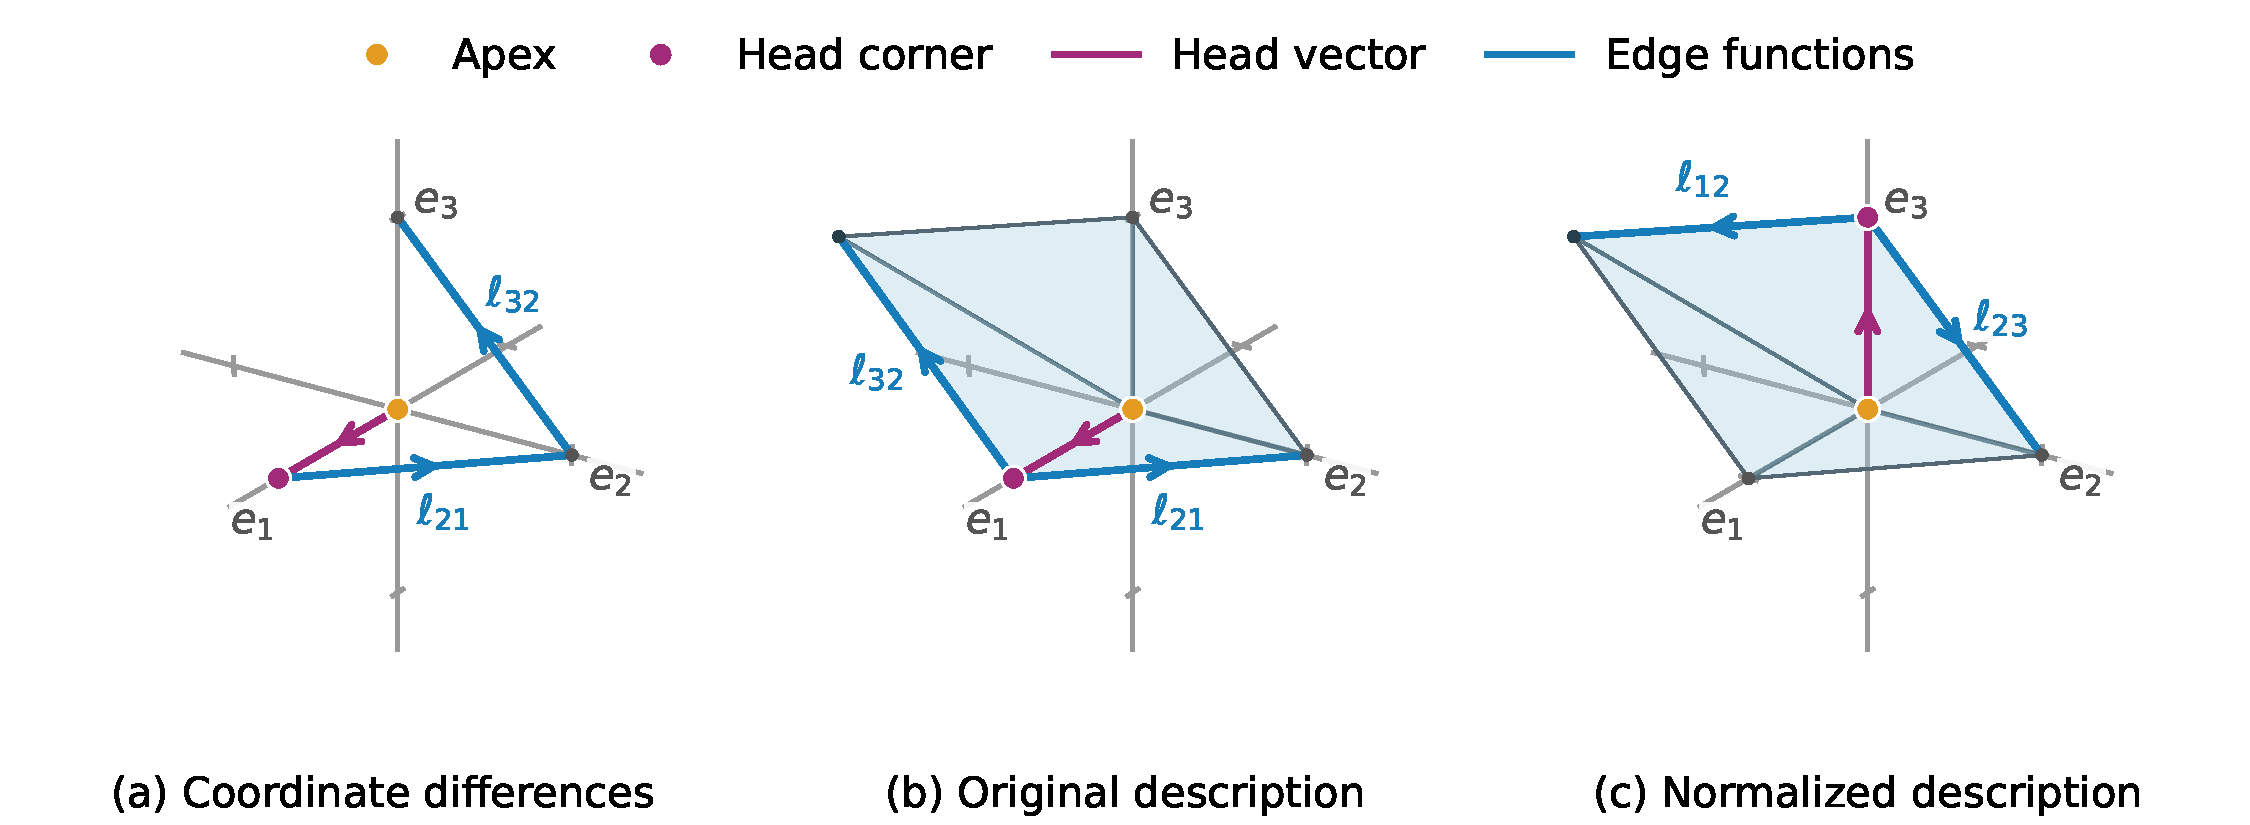
\includegraphics[width=\textwidth]{figures/caterpillar-normalization.pdf}
\caption{Coordinate differences and the caterpillar polytope for $\pi=(0,3,2,1)$ and $S=\{1,2\}$. (a) The head $h=e_1-e_0$ and edge functions $L=\{\ell_{32}=e_3-e_2,\ell_{21}=e_2-e_1\}$ drawn between their labelled endpoints. (b) The same generators translated to the base corner $h$ of $Q_{h,L}$. (c) Normalization (\Cref{sec:size}) gives $h^+=h+\ell_{32}+\ell_{21}=e_3-e_0$ and $L^+=\{\ell_{12}=e_1-e_2,\ell_{23}=e_2-e_3\}$, leaving the polytope unchanged. Purple arrows represent the head (the apex--last spine connection before normalization); blue arrows represent the spine edge functions. Orange dots mark the polytope apex and purple dots the chosen head corner. The grey coordinate axes meet at the origin, representing $e_0$ after restriction to $x_0=0$; the positive unit points are labelled $e_1,e_2,e_3$.}
\label{fig:polytope-normalization}
\end{figure}

\begin{Proof}{Theorem}{thm:main}
Fix $N\geq3$. We bound the quotient dimension $q_N$ of \Cref{sec:compression}
by the count of normalized descriptions and apply
\Cref{thm:quotient-compression}.

\pfstep{stp:size-count}{Count the caterpillar face functions}
Use the adjusted heads and normalized descriptions from \Cref{sec:size}. Counting distinct normalized descriptions bounds $q_N$.

For a caterpillar description $(\pi,S)$, the spine endpoints are labelled $\pi(1)$ and $\pi(q+1)$, and every label other than $\pi(1)$ and the apex is the child of exactly one edge. Hence the normalized description of $U_{\pi,S}$ is
\begin{align}\label{eq:graph}
\begin{split}
h_{\pi,S}^+(x)&=\sum_{\ell_{ij}\in L_{\pi,S}}x_{\max(i,j)}+x_{\pi(1)}+x_{\pi(q+1)}
-\sum_{i=0}^{N-1}x_i,\\
L_{\pi,S}^+&=\{\ell_{\min(i,j),\max(i,j)}:\ell_{ij}\in L_{\pi,S}\}.
\end{split}
\end{align}
This depends only on the undirected tree, apex, and unordered spine
endpoints. For $m$ spine vertices, choose the vertex set in $\binom Nm$
ways, its order up to reversal in $m!/2$ ways, the apex in $N-m$ ways,
and each of the $N-m-1$ leaf attachments in $m$ ways. Reversal has no
fixed point since $m\geq2$, so~\Cref{eq:count} gives
\begin{align}\label{eq:cone-count}
 \bigl|\{(h^+_{\pi,S},L^+_{\pi,S}):(\pi,S)\text{ a caterpillar description}\}\bigr|\leq C_N.
\end{align}

Reversing an edge swaps its omitted and linear states. Thus choosing
states before or after normalization gives the same family
$\mathcal K_0$ of descriptions, with $|\mathcal K_0|\leq3^{N-2}C_N$.
Write $U_k:=U_{h,M}$ for $k=(h,M)$. We merge equal descriptions;
distinct descriptions may still represent the same function.

Among them are the descriptions $(\ell_{ij},\varnothing)$ representing $x\mapsto\relu(x_i-x_j)$, with $i\ne j$: for the all-cut path $S=\{1,\ldots,r\}$ with apex $\pi(0)=j$ and last spine vertex $\pi(r+1)=i$, omitting every edge function gives
\begin{align}\label{eq:absorbed-pairs}
 U^{0}_{\pi,S}=\relu\circ\ell_{ij}\qquad(0\leq i\ne j<N).
\end{align}
Let $\mathcal P\subseteq\mathcal K_0$ consist of descriptions with empty
hinge set and head a coordinate difference. The distinct heads
$\ell_{ij}$ give $|\mathcal P|\geq N(N-1)$. Put
\begin{align}\label{eq:retained-descriptions}
 K:=\mathcal K_0\setminus\mathcal P.
\end{align}
Every face function in $\D$ equals $U_k$ for its normalized description
$k\in\mathcal K_0$, and by~\Cref{eq:hinge-reversal} every unit indexed by
$\mathcal P$ lies in the auxiliary span $A_N$. Hence the units $U_k$,
$k\in K$, span $V_N$ modulo $A_N$, and
\begin{align}\label{eq:retained-count}
q_N\leq|K|\leq3^{N-2}C_N-N(N-1).
\end{align}

\pfstep{stp:size-network}{Compile the network and establish its widths}
\Cref{thm:quotient-compression} gives a network with rational weights, zero
biases, first width $h_1$, and second width
\begin{align}\label{eq:compilation-widths}
q_N+2\leq3^{N-2}C_N-N(N-1)+2=h_2.
\end{align}
Zero padding realizes the stated widths exactly.

For the growth rates, count the ordered choices of $m$ spine labels:
\begin{align}\label{eq:head-count-bound}
\binom Nm\frac{m!}{2}=\frac{N!}{2(N-m)!}\leq N^m\qquad(2\leq m\leq N-1).
\end{align}
Using $N-m\leq N$ and $m^{N-m-1}\leq N^{N-m-1}$ in each summand of~\Cref{eq:count} gives
\begin{align}\label{eq:cone-growth}
\begin{aligned}
C_N&\leq\sum_{m=2}^{N-1}N^m\,N\,N^{N-m-1}=(N-2)N^N\\
&\leq N^{N+1}\leq N^{4N}.
\end{aligned}
\end{align}
Since $3^{N-2}\leq N^N$ for $N\geq3$,
\begin{align}
h_2&\leq3^{N-2}(N-2)N^N+2\leq2N^{5N},\label{eq:second-growth}\\
h_1&\leq4N^2.\label{eq:first-growth}
\end{align}
Taking logarithms gives the asymptotic bounds in~\Cref{thm:main}.
\end{Proof}
% End appendices/widths.tex
% Begin appendices/lower.tex
\section{Proofs of the lower bounds}\label{app:lower}

\subsection{Proof of the exponential count bound}\label{app:count-exponential}

We prove \Cref{thm:forest-count} and obtain
\Crefrange{eq:count-binomial}{eq:count-exponential} by taking $\Delta=2$.
The proof uses one mixed difference and a product over disjoint star blocks.

\begin{Proof}{Theorem}{thm:count-exponential}
\phantomsection\label[proof]{pf:thm:forest-count}
Fix an expansion as in \Cref{thm:forest-count}, and $3\leq m\leq N$.
Write $U_k=\relu(A_k)$ with
$A_k(x)=\sum_o h_{k,o}x_o+\sum_{(i,j)\in M_k}\relu(x_i-x_j)$.
Reorienting edges by \Cref{eq:hinge-reversal} preserves $A_k$ and
$\kappa_{k,o}$, so we may assume $i<j$ in $M_k$.
Choose an integer $B>1$ and $\delta>0$ such that, for every $k$,
$B>\sum_o|h_{k,o}|+|M_k|$ and
$\delta(\sum_o|h_{k,o}|+2|M_k|)<1$.

\pfstep{stp:count-functional}{A mixed difference detects every top tie}
A permutation $\rho$ assigns positions to labels, with smaller positions
higher. Put $T_\rho=\{o:\rho(o)<m\}$ and define
\begin{align}
 p^\rho_o&=\begin{cases}0,&o\in T_\rho,\\-B^{\rho(o)},&o\notin T_\rho,\end{cases}\label{eq:base-point}\\
 \Delta_\rho g&=\sum_{S\subseteq T_\rho}(-1)^{m-|S|}
                 g(p^\rho+\delta\one_S).\label{eq:mixed-difference}
\end{align}
Pairing corners along a missing coordinate shows that $\Delta_\rho$
annihilates every function of at most two coordinates. On this cube the
maximum is $\delta$ at every nonempty corner and $0$ at the empty corner.
Thus
\begin{align}
 \Delta_\rho R&=0\qquad(R\in A_N),\label{eq:mixed-auxiliary}\\
 \Delta_\rho\maxn_N&=(-1)^{m+1}\delta\ne0.\label{eq:mixed-maximum}
\end{align}
Some $U_k$ in the expansion therefore satisfies $\Delta_\rho U_k\ne0$.

\pfstep{stp:count-digits}{Detection forces balance}
Fix one such unit and suppress its index. Its preactivation at $p^\rho$
is an integer and changes by less than $1$ on the cube. Unless $A(p^\rho)=0$,
its outer ReLU is either zero or redundant throughout the cube, and
$\Delta_\rho U=0$.
For $o\notin T_\rho$, let $u_\rho(o)$ count its neighbours at smaller
positions. Collecting coefficients gives
\begin{align}\label{eq:preactivation-digits}
 A(p^\rho)=-\sum_{o\notin T_\rho}(\kappa_o-u_\rho(o))B^{\rho(o)}.
\end{align}
The integer digits have absolute value less than $B$. Successively reducing
modulo $B$ forces each digit to vanish.
Moreover, if a tied label $t$ has no tied neighbour, the slope in $x_t$ on
the cube is $\kappa_t$; if this is zero, the mixed difference vanishes.
Call $U$ \emph{passing} $\rho$ when these two necessary conditions hold:
\begin{align}
 u_\rho(o)&=\kappa_o&&\text{for }o\notin T_\rho,\label{eq:balanced}\\
 \kappa_t&\ne0&&\text{for }t\in T_\rho\text{ with no neighbour in }T_\rho.\label{eq:active}
\end{align}
Every permutation is passed by some unit in the expansion.

\pfstep{stp:count-admissible}{Only the reduced forest chooses the tie set}
Fix a unit, let $F$ be its forest, and call the deleted degree-one vertices
\emph{pendants}. Let $\Phi$ contain the vertices that are neither pendants
nor isolated in $F$. For a passed tie set $T$, an isolated vertex belongs
to $T$ exactly when its $\kappa$ is nonzero. A pendant belongs to $T$ exactly
when its neighbour does: either mismatch contradicts
\Cref{eq:balanced,eq:active}. A component consisting of two pendants must
lie entirely in $T$, since otherwise its lower vertex violates balance.
Consequently $T$ is determined by $A=T\cap\Phi$, and $|A|\leq m$.

\pfstep{stp:count-orders}{Each disjoint edge halves the possible orders}
For fixed $T$, balance prescribes the out-degree of each vertex of $F-T$
when edges point towards the higher endpoint. A forest orientation is
uniquely determined by its out-degrees: orient the edge at a leaf, delete
the leaf, and repeat. Hence every passed permutation with this $T$ induces
the same orientation of $F-T$.
If we select a matching of $\mu(A)$ edges of $F-T$, independently swapping
their endpoints gives
\begin{align}\label{eq:order-count}
 |\{\rho:U\text{ passes }\rho,\ T_\rho=T\}|
 \leq m!\,(N-m)!\,2^{-\mu(A)}.
\end{align}

\pfstep{stp:count-transfer}{Partition into blocks and multiply their weights}
Partition $\Phi$ into stars of the reduced forest and singletons isolated
in that forest. Such a star partition exists: an inclusion-minimal edge
cover of the non-isolated vertices contains no three-edge path, since its
middle edge could be removed. As it is a forest, its components are stars.
Every star has $1\leq s\leq\Delta$ leaves. A singleton has a pendant
neighbour in $F$; fix one.

For $A\subseteq\Phi$, select one edge in a star block whenever its centre
and some leaf are outside $A$. At a singleton outside $A$, select its fixed
pendant edge. For a passed tie set these are disjoint edges of $F-T$.
Let $\mu(A)$ count them and put $y=1/(2\Delta+2)=1/b$.
The sum of $y^{|A|}2^{-\mu(A)}$ factorizes over blocks. A singleton has
weight $1/2+y$; a star with $s$ leaves has weight
\begin{align}\label{eq:block-weight}
 W_s(y)=y(1+y)^s+\tfrac12\bigl((1+y)^s-y^s\bigr)+y^s
       =(\tfrac12+y)(1+y)^s+\tfrac12y^s.
\end{align}
The three terms distinguish a selected centre, an unselected centre with
an unselected leaf, and an unselected centre with all leaves selected.
All block weights are at most $1$. For $\Delta=2$, the singleton, one-leaf,
and two-leaf weights at $y=1/6$ are respectively
$2/3$, $31/36$, and $199/216$.
In general $y\leq1/6$; the one-leaf case is bounded by $31/36$, and for
$2\leq s\leq\Delta$,
$W_s(y)\leq(1/2+y)e^{1/2-y}+y^2/2
\leq(2/3)e^{1/3}+1/72<1$.
Thus
\begin{align}\label{eq:path-weight}
 \sum_{A\subseteq\Phi}y^{|A|}2^{-\mu(A)}
 =\prod_{\text{blocks}}W_{\text{block}}(y)\leq1.
\end{align}

\pfstep{stp:count-assembly}{Count all permutations}
Distinct passed tie sets have distinct $A=T\cap\Phi$, and $|A|\leq m$.
Summing \Cref{eq:order-count} and inserting the factor
$1\leq b^m y^{|A|}$ bounds the number of permutations passed by one unit by
$m!\,(N-m)!\,b^m$ using \Cref{eq:path-weight}.
The units cover all $N!$ permutations, so
$N!\leq |K|\,m!\,(N-m)!\,b^m$, proving \Cref{eq:forest-count}.
Caterpillar functions have reduced degree at most $2$, giving
\Cref{eq:count-binomial}.

\pfstep{stp:count-corollary}{Extract the exponential bound}
Put $t_m=\binom Nm b^{-m}$. If $N\geq3b+2$, then
$t_0\leq t_1\leq t_2\leq t_3$, so every $t_m$ is at most $|K|$.
The binomial theorem gives
\begin{align}\label{eq:binomial-sum}
 (1+1/b)^N=\sum_{m=0}^N t_m\leq(N+1)|K|.
\end{align}
For $b=6$ and $3\leq N<20$, the same conclusion follows from
$|K|\geq1$ and $(7/6)^N\leq N+1$.
This proves \Cref{eq:count-exponential} and the remaining assertions of
\Cref{thm:forest-count}.
\paragraph[Quadratic refinement]{Quadratic refinement (\leandecl{MaxCaterpillar/CountLower.lean}{124}{caterpillar_count_lower}).}
The bound \Cref{eq:count-quadratic} uses
three-element tie sets, a six-point second difference, and the sharper
count of at most $N-2$ tie sets per caterpillar function.
\end{Proof}

\Needspace{8\baselineskip}
\begin{Proof}{Theorem}{thm:degree-two-weighted}
First remove biases, if present, by taking the recession function
$\lim_{t\to\infty}F(tx)/t$. This preserves the homogeneous target, the
comparison graphs, and the number of neurons.

Fix an $m$-element label set $T$. Take the directional germ at $\one_T$,
vary only the tied coordinates, and fix one tied perturbation coordinate
to zero. The target germ is the support function of an $(m-1)$-simplex,
whose class modulo $\LS_{m-2}$ is nonzero. Indeed, repeated opposite-face
differences and restrictions to facet coordinates would otherwise, by
\Cref{eq:face-dimension-drop}, put a segment support function in $\LS_0$;
that function is not linear. The germ of the shallow remainder lies in
$\LS_1$.

For a counted unit, only comparisons with both endpoints in $T$ remain
nonlinear. Let $c$ be the number of connected components of its induced
comparison graph, including isolated vertices. The free comparison forms
span a space of dimension $m-c$. If the outer preactivation is nonzero at
$\one_T$, the germ is zero or belongs to $\LS_1$. Otherwise, adjoining the
resulting linear head gives at most $m-c+1$ directions. Signed inner weights
cause no difficulty: split the local preactivation as $h_P-h_Q$, where the
two polytopes lie in this span, and use
$\relu(h_P-h_Q)=h_{\operatorname{conv}(P\cup Q)}-h_Q$.
Thus its germ belongs to $\LS_{m-c+1}$. If $c\geq3$, its class modulo
$\LS_{m-2}$ vanishes. Every tie therefore requires some counted unit whose
induced graph has at most two connected components.

For a graph of maximum degree two, let $C_j$ count its connected induced
$j$-vertex subsets. Each path or cycle component contributes at most its
number of vertices: a proper connected subset is an interval or circular
arc, and a whole component contributes only once. Hence $C_j\leq N$.
An $m$-element set with two induced components is an unordered union of
two connected sets. Dropping disjointness and the absence of edges between
them only increases the count. A single unit consequently covers at most
\begin{align}\label{eq:degree-two-capacity}
 C_m+\frac12\sum_{j=1}^{m-1}C_jC_{m-j}
 \leq N+\frac{m-1}{2}N^2
\end{align}
ties of size $m$. Counting all $\binom Nm$ ties proves
\Cref{eq:degree-two-count}. The central binomial coefficient is
$\Theta(2^N/\sqrt N)$, giving the stated asymptotic bound.
\end{Proof}

\Needspace{8\baselineskip}
\begin{Proof}{Theorem}{thm:weighted-forest}
The locality argument in the proof of \Cref{thm:degree-two-weighted} shows that every
label set $T$ with $|T|\geq3$ needs a comparison graph $G$ for which $G[T]$
has at most two components. Give a pseudoforest $G$ an auxiliary orientation
of indegree at most one: orient tree components away from a root, cycles
cyclically, and attached trees away from the cycle. This orientation is
independent of the ReLU orientations. Every connected induced subgraph has
at most one vertex of indegree zero, since their number is $|V|-|E|$.
Fix a matching. If a matched parent is absent from $T$ and its child is
present, that child has indegree zero in $G[T]$. Different matching edges
therefore give different components. With independent vertex selection
of probability $p$, these events are independent and have probability
$p(1-p)$. Thus, for a matching of size $k$ and $\rho=1-p(1-p)$,
\begin{align}\label{eq:matching-witnesses}
 \Pr\bigl(c(G[T])\leq2\bigr)
 \leq\rho^k\left(1+k\frac{1-\rho}{\rho}
             +\binom k2\left(\frac{1-\rho}{\rho}\right)^2\right).
\end{align}

At $p=1/2$, selected isolated vertices give additional independent component
witnesses of probability $1/2$, on labels disjoint from the matching.
Replacing their probability by $1/4$ only increases the probability of at
most two witnesses. A pseudoforest with $\nu(G)+z(G)\geq k$ therefore serves at
most a fraction $(3/4)^k c_k$ of all subsets. Since
$\Pr(|T|\geq3)=1-b_N2^{-N}$, the union bound proves
\Cref{eq:weighted-forest-count}.

For the degree bound, fix a maximum matching in any graph of maximum degree
$\Delta\geq2$. Unmatched vertices are independent. The two endpoints of a
matched edge cannot have distinct unmatched neighbors, since those four
vertices would give an augmenting path. Hence each matched edge has at
most $\Delta-1$ distinct unmatched neighbors: either all attach to one
endpoint, or both endpoints share a single unmatched neighbor. Every
nonisolated unmatched vertex attaches to a matched edge, so
$N-z(G)-2\nu(G)\leq(\Delta-1)\nu(G)$.
Thus $\nu(G)+z(G)\geq\lceil N/(\Delta+1)\rceil$; degrees zero and one
are immediate.

For general graphs of bounded degree, put $r=\Delta+1$ and select labels
independently with probability $1/r$. Let $Z_v$ indicate that $v$ is selected
and isolated in $G[T]$. Then $\Pr(Z_v=1)\geq q_\Delta$, and each input bit
affects at most $r$ of these indicators. The product inequality
$\mathbb E\prod_v f_v\leq\prod_v(\mathbb E f_v^r)^{1/r}$ applies whenever
each independent input occurs in at most $r$ nonnegative factors.
To prove it, condition on all but one input, apply H\"older to the incident
factors, and induct on the remaining inputs. This also gives the usual
concentration bound for this dependence pattern~\cite{GavinskyEtAl}.

Apply the inequality with $f_v=\exp(-tZ_v)$ to obtain
$\mathbb E\exp(-t\sum_v Z_v)\leq(1-q_\Delta+q_\Delta e^{-rt})^{N/r}$.
Since $c(G[T])\leq2$ forces $\sum_v Z_v\leq2$, exponential Markov with
$t=(\log N)/r$ gives
\begin{align}\label{eq:weighted-isolates}
 \Pr\bigl(c(G[T])\leq2\bigr)
 \leq N^{2/r}(1-q_\Delta+q_\Delta/N)^{N/r}
 =O_\Delta\bigl(N^{2/r}(1-q_\Delta)^{N/r}\bigr).
\end{align}
Now $\Pr(|T|\geq3)\to1$, so the same union bound proves the stated estimate.
Repeating a graph with different heads and weights
adds no tied sets to its coverage, so these bounds also count distinct graphs.
\end{Proof}

For \Cref{eq:bounded-excess-count}, extend a maximum matching of $G$ to a
spanning forest, then add one omitted edge in each originally cyclic
component. The resulting pseudoforest $P$ preserves the matching and all
isolated vertices, and omits exactly $b(G)$ edges. Restoring an edge merges
at most two induced components, so $c(G[T])\geq c(P[T])-b(G)$.
The independent matching and isolate witnesses in the preceding proof
therefore show that $c(G[T])\leq2$ requires at most $b+2$ successes in a
binomial variable with parameters $k$ and $1/4$. Apply the same union bound.
The exponential conclusions follow from the binomial lower-tail estimate;
when $b=o(k)$ its probability is at most
$\exp[-(\log(4/3)-o(1))k]$.

\paragraph{Arbitrary tree shapes with a source orientation.}
The block argument also works with a subforest $R$ of the reduced forest:
its maximum degree must be at most two, and each vertex of $\Phi$ isolated
in $R$ must either have a pendant neighbour or belong to every passed tie
set. Use the same star partition of $R$. The first kind of singleton has
weight $1/2+y$; the second has weight $y$, since it must be selected.
All weights are at most one at $y=1/6$, so the same counting argument applies.
A leaf with $\kappa\notin\{0,1\}$ is always tied: otherwise balance would
require its unique edge to give an out-degree other than zero or one.

For $U_{a,s,r,T}$, root the underlying tree at the head root $r$.
Call a nonleaf \emph{poor} if it has neither a pendant nor an out-leaf
neighbour. Choose one child of each poor vertex; such a child exists, and
no child is chosen by two parents. Let $R$ contain these chosen edges,
together with every edge from an out-leaf to a nonpendant neighbour.
These edges belong to the reduced forest. An isolated vertex of $R$ in $\Phi$ is
either adjacent to a pendant or a leaf with $\kappa\notin\{0,1\}$, so it
satisfies the required condition.

Leaves have degree at most one in $R$. A nonleaf with at most one out-leaf
neighbour has degree at most two in $R$:
a poor vertex contributes one chosen child edge and can receive one, whereas
any other vertex receives at most one chosen child edge. The only remaining
case is a common neighbour $v$ of the two out-leaves $s$ and $r$.
It is not poor. Its parent is the leaf $r$, which is not poor either, so
no chosen child edge ends at $v$. Its only $R$-edges are the two out-leaf
edges. Thus $R$ has maximum degree two. This gives the per-unit factor $6^m$
for every $U_{a,s,r,T}$, and hence the stated $(7/6)^N/(N+1)$ bound for mixtures
with the existing caterpillar and rooted-star face dictionaries.

\paragraph{Large matchings with arbitrary heads and weights.}
Let $K_0$ count the caterpillar and rooted-star face functions, and $K_1$
the added weighted-pseudoforest functions with matching number at least $k$.
At each permutation locality, some unit has a nonzero top class. The base
functions contribute at most $6^m m!(N-m)!$ localities of size $m$.
For the added functions, the rank argument in
\Cref{thm:weighted-forest} requires at most two induced components;
\Cref{eq:matching-witnesses} bounds their weighted coverage independently
of the heads, coefficients, and outside order.

Divide by $m!(N-m)!$, multiply by $y^m$, and sum over $3\leq m\leq N$.
Take $y=2/11$, so $p=y/(1+y)=2/13$ and $\rho=147/169$, and put
\[
 E=(13/11)^N\rho^k,\qquad
 d_k=1+\frac{22}{147}k+\left(\frac{22}{147}\right)^2\binom k2,
 \qquad Z=|K_0|+|K_1|.
\]
Each added function contributes at most $E d_k$, whereas each base
function contributes at most $(N-2)(12/11)^N$. Since $2k\leq N$ and
$147\geq144$, we have $E\geq(12/11)^N\geq1$.
Also $Z\geq1$, since auxiliary functions cannot supply a three-label
simplex germ. Consequently coverage gives
\[
 (13/11)^N\leq
 \left(1+\frac{2N}{11}+\frac4{121}\binom N2+N-2+d_k\right)EZ
 \leq(N+1)^2 EZ.
\]
For the last inequality, bound the first three terms and $d_k$ separately
by $1+N/2+N^2/8$; the resulting bracket is at most $2N+N^2/4$.
Canceling $(13/11)^N$ proves $Z\geq(169/147)^k/(N+1)^2$.
Finally, for a tree on $n$ vertices, the leaf criterion follows from a minimum vertex cover $C$ of
size equal to the maximum matching number $\nu$. The nonleaf vertices
outside $C$ form an independent set $I$; their at least $2|I|$ incident
edges lie in the forest on $I\cup C$, which has at most $|I|+\nu-1$
edges. Hence $|I|\leq\nu-1$, and $n-L\leq2\nu-1$.

\paragraph{Adding every oriented star.}
Work in full coordinates. For a label $j$, let $\iota_j$ insert a zero at
that coordinate and put
$\mathcal T_j g=(\partial_{-e_j}g-\partial_{e_j}g)\circ\iota_j$.
This linear operator sends $\LS_d$ into $\LS_{d-1}$ for $d\geq1$ and
annihilates $\LS_0$: if coordinate $j$ is constant on a polytope, its two
exposed faces coincide; otherwise both have smaller dimension. Projection
under restriction cannot increase dimension. Moreover,
$\mathcal T_j\maxn_m=\maxn_{m-1}$, since the simplex faces are its facet
opposite $e_j$ and the vertex $e_j$.

For a canonical star, deletion of a nonroot leaf gives the smaller star
modulo $\LS_1$, with sign $+$ for $\relu(x_l-x_c)$ and sign $-$ for
$\relu(x_c-x_l)$. If the deleted leaf is the head root, the latter
orientation transfers the head to the centre with sign $+$; the former
gives zero modulo $\LS_1$. Deleting the apex leaves a zonotope, and deleting
the centre fixes every segment, so these cases also give zero modulo
$\LS_1$. Thus successive deletions preserve the span of canonical stars
modulo the lower-dimensional terms.

At five labels, a
\href{\leanbase/research/sN/trees/all_tree_dfs/complete_flags_5.json}{six-flag certificate}
gives a linear functional that annihilates every canonical oriented star
and $\LS_3$, and takes value $120$ on the simplex. The
\href{\leanbase/research/sN/trees/dfs_review_flag_certificate.py}{independent vertex checker}
checks all $640$ labelled stars, with every head root and orientation,
by successive maxima and minima over explicit vertex sets. Composing
this functional with $m-5$ coordinate deletions therefore gives such a
separator at every $m\geq5$. A nonhinge state already has dimension at
most $m-2$, so all star face states are covered too.

Assign every term whose function belongs to the star family to the added
star class, even if it was originally listed in another class. Here
$K_0,K_1$ count only the remaining terms, and $Z=|K_0|+|K_1|$.
At any tie of size at least five, a surviving top-dimensional star germ is again a canonical
star: each untied component has a unique attachment to the tied subtree,
and summing its zero frozen coefficients transports the head to that
attachment if it contains the original root. Apply the separator to
the local expansion. Every added star term vanishes, so a term from the
other classes must cover the locality. The preceding weighted count now
starts at $m=5$. With caterpillars alone, $y=1/6$ gives
$(7/6)^N-\sum_{j=0}^4\binom Nj6^{-j}\leq(N-4)|K_0|$.
There is at least one nonstar term, and
$\sum_{j=0}^4\binom Nj6^{-j}+N-4\leq(N+1)^4$ for $N\geq5$,
which proves the first assertion. For the matching class, the same
choice $y=2/11$ and the same $E$ as above give
$(13/11)^N\leq
\bigl(\sum_{j=0}^4\binom Nj(2/11)^j+N-4+d_k\bigr)EZ
\leq(N+1)^4EZ$.
This proves the stated bound without counting the added star terms.

\subsection{Proof of the dimension bound}\label{app:quotient-lower}

\begin{Proof}{Theorem}{thm:quotient-lower}
Put $r=N-2$ and $b=N-1$. We exhibit $r!$ dictionary functions and linear
functionals whose evaluation matrix is the identity and which annihilate
$A_N$.

\pfstep{stp:quotient-path-units}{One path for each order}
For every permutation $\pi$ fixing $0$ and $b$, use the path
$\pi(1),\ldots,\pi(r),b$ with apex $0$ and keep every edge as a hinge:
\begin{align}\label{eq:path-unit}
 U_\pi(x)=\relu\Bigl(x_b-x_0+
   \sum_{j=1}^{r}\relu(x_{\pi(j)}-x_{\pi(j+1)})\Bigr)\in V_N.
\end{align}
There are $r!$ such paths.

\pfstep{stp:quotient-auxiliary}{One mixed difference}
For an order $\rho$, set $c=\rho(r)$ and
\begin{align}\label{eq:test-configuration}
 z^\rho_0=z^\rho_b=2r,\qquad z^\rho_{\rho(j)}=2j\quad(1\leq j\leq r).
\end{align}
Thus $0,b,c$ tie at the top. Let
$\Lambda_\rho g=\sum_{S\subseteq\{0,b,c\}}(-1)^{3-|S|}g(z^\rho+\one_S)$.
This third mixed difference annihilates every function of at most two
coordinates, by pairing corners along a missing coordinate. In particular,
$\Lambda_\rho A_N=0$.

\pfstep{stp:quotient-path-values}{The evaluation matrix is the identity}
On the cube of $\Lambda_\rho$, every inner function of $U_\rho$ except the
last is zero: adjacent base heights differ by $2$, while a coordinate moves
by at most $1$. Writing $v=x-z^\rho$, we obtain
$U_\rho=\relu(v_b-v_0+\relu(v_c-v_b))$.
At the eight corners this is $1$ exactly when $v_0=0$ and
$(v_b,v_c)\ne(0,0)$, so its mixed difference is $1+1-1=1$.

If $\pi\ne\rho$, the middle labels in the $\pi$-order have a descent in
$\rho$-height. The corresponding inner function is at least $1$ everywhere
on the cube, whereas $x_b-x_0\geq-1$. The outer ReLU can therefore be removed
there. The resulting sum depends on at most two coordinates term by term,
so its third mixed difference is zero. Hence
\begin{align}\label{eq:path-functional}
 \Lambda_\rho U_\pi=\begin{cases}1,&\pi=\rho,\\0,&\pi\ne\rho.\end{cases}
\end{align}

\pfstep{stp:quotient-independence}{Independence modulo the auxiliary span}
Applying $\Lambda_\rho$ to $\sum_\pi c_\pi U_\pi\in A_N$ gives $c_\rho=0$.
Thus these $r!$ functions are independent modulo $A_N$, proving
$q_N\geq(N-2)!$.
\end{Proof}
% End appendices/lower.tex
% Begin appendices/lean.tex
\section{Relation to the construction of Brunck et al.}\label{app:bsy}

The combinatorial proof of \cite[Part~2]{BSY} cones zonotopes
$B_{v,\pi,M}$ to pyramids and expresses the simplex support function as a
signed sum of their support functions modulo lower-dimensional terms
\cite[Lemma~22]{BSY}. This appendix identifies these building blocks. For a
nonempty set $M$ of marked positions, the pyramid has the support function
of a translated caterpillar polytope, with apex $v$, label order $\pi$, and
cut set $M-1$. For $M=\varnothing$ it gives a rooted star, which is not a
caterpillar function. We use the indexing of \cite[Section~7.1]{BSY}, with
their $n$ written as $N$ and $[N]$ identified with our label set
$\{0,\ldots,N-1\}$. Positions of an ordering are numbered from $1$.

\Needspace{12\baselineskip}
\begin{definition}[Zonotopes of Brunck et al., \leandecl{MaxCaterpillar/Competing/Defs.lean}{78}{parallelepiped}, \leandecl{MaxCaterpillar/Competing/Defs.lean}{88}{paramidSupport}]\label{def:bsy}
Let $N\geq3$, let $v$ be a label, let $\pi=(\pi_1,\ldots,\pi_{N-1})$ be an
ordering of the remaining labels, and let $M\subseteq\{2,\ldots,N-1\}$.
For $p\in\R^N$ put $u_i(p):=\sum_{1\leq j<i}p_{\pi_j}$. Following
\cite[Equation~(3)]{BSY}, define
\begin{align}
 H_{-v}&:=\Bigl\{p\in\R^N:p_v=0,\ \sum_kp_k=1\Bigr\},\label{eq:bsy-hyperplane}\\
 B_{v,\pi,M}&:=\left\{p\in H_{-v}:
 \begin{array}{ll}
 0\leq u_i(p)\leq1 & \text{for } i\in M,\\
 -1\leq p_{\pi_i}\leq0 & \text{for } i\in\{2,\ldots,N-1\}\setminus M
 \end{array}\right\}.\label{eq:bsy-parallelepiped}
\end{align}
The pyramid with apex $e_v$ is
$\operatorname{pyr}_{e_v}(B_{v,\pi,M}):=\operatorname{conv}(\{e_v\}\cup
B_{v,\pi,M})$, with support function $h_{v,\pi,M}$ as
in~\Cref{eq:support-function}. Its last marked position and the marked
parent of a position $i$ are
\begin{align}\label{eq:bsy-marked}
 q:=\max(\{1\}\cup M),\qquad
 r(i):=\max\bigl(\{1\}\cup\{j\in M:j<i\}\bigr)\qquad(2\leq i\leq N-1).
\end{align}
For $M\neq\varnothing$, $q=\max M$. For labels $a\neq c$, the \emph{rooted
star} with apex $a$ and root $c$ is
\begin{align}\label{eq:rooted-star}
 S_{a,c}(x):=\relu\Bigl(x_c-x_a+\sum_{l\notin\{a,c\}}\relu(x_c-x_l)\Bigr).
\end{align}
\end{definition}

\Needspace{12\baselineskip}
\begin{theorem}[Relation to Brunck et al., \leandecl{MaxCaterpillar/Theorems.lean}{203}{bhrsy_parallelepiped_eq_zonotope}, \leandecl{MaxCaterpillar/Theorems.lean}{231}{bhrsy_support_eq}, \leandecl{MaxCaterpillar/Theorems.lean}{240}{bhrsy_support_eq_word}, \leandecl{MaxCaterpillar/Theorems.lean}{249}{bhrsy_support_mem_caterpillar}, \leandecl{MaxCaterpillar/Theorems.lean}{258}{bhrsy_word_mem}, \leandecl{MaxCaterpillar/Theorems.lean}{269}{bhrsy_support_empty}, \leandecl{MaxCaterpillar/Theorems.lean}{275}{rootedStar_ne_caterpillarFunction}, \leandecl{MaxCaterpillar/Theorems.lean}{289}{bhrsy_family}, {\Cref{pf:thm:bsy-relation}}]\label{thm:bsy-relation}
Let $v$, $\pi$, and $M$ be as in~\Cref{def:bsy}, and let $q$ and $r(i)$ be as
in~\Cref{eq:bsy-marked}.
\begin{enumerate}
\item[(a)] The base is the zonotope
\begin{align}\label{eq:bsy-zonotope}
 B_{v,\pi,M}=e_{\pi_q}+\sum_{i=2}^{N-1}\bigl[0,e_{\pi_{r(i)}}-e_{\pi_i}\bigr].
\end{align}
\item[(b)] For every $x\in\R^N$,
\begin{align}\label{eq:bsy-support}
 h_{v,\pi,M}(x)=x_v+\relu\Bigl(x_{\pi_q}-x_v+\sum_{i=2}^{N-1}\relu\bigl(x_{\pi_{r(i)}}-x_{\pi_i}\bigr)\Bigr).
\end{align}
\item[(c)] Let $M\neq\varnothing$. Define the caterpillar description $(\pi',S)$
by $\pi'(0):=v$, $\pi'(j):=\pi_j$ for $1\leq j\leq N-1$, and
$S:=\{i-1:i\in M\}$. Then $|S|=|M|$ and
\begin{align}\label{eq:bsy-word}
 h_{v,\pi,M}(x)=x_v+U_{\pi',S}(x)\qquad(x\in\R^N).
\end{align}
Hence $h_{v,\pi,M}-x_v=U_k$ for some $k\in\mathcal K_0$. Conversely, every
caterpillar description $(\pi',S)$ arises in this way from $v=\pi'(0)$,
$\pi_j=\pi'(j)$, and $M=\{j+1:j\in S\}\neq\varnothing$.
\item[(d)] Let $M=\varnothing$. Then $h_{v,\pi,\varnothing}(x)=x_v+S_{v,\pi_1}(x)$.
No rooted star is a caterpillar function: $S_{a,c}\neq U_k$ for all labels
$a\neq c$ and all $k\in\mathcal K_0$. In particular,
$h_{v,\pi,\varnothing}-x_v\neq U_k$ for every $k\in\mathcal K_0$.
\end{enumerate}
\end{theorem}
By~\Cref{eq:unit-polytope}, the right-hand side of~\Cref{eq:bsy-word} is
the support function of the translated caterpillar polytope
$e_v+Q_{h_{\pi',S},L_{\pi',S}}$. The family of \cite{BSY} therefore consists
of the caterpillar polytopes, translated by $e_v$, and of the pyramids over
rooted stars. The sign $(-1)^{|M|}$ of \cite[Lemma~22]{BSY} equals
$(-1)^{|S|}$. The theorem compares building blocks only. It makes no
statement about corrections or network coefficients.

\begin{Proof}{Theorem}{thm:bsy-relation}
Write $I:=\{2,\ldots,N-1\}$ and $g_i:=e_{\pi_{r(i)}}-e_{\pi_i}$ for $i\in I$.
Every element of $\{1\}\cup M$ lies in $\{1,\ldots,N-1\}$, so $q$ and all
$r(i)$ are positions. Since $M\subseteq I$, the definitions give
\begin{itemize}
\item $1\leq r(i)<i$ for $i\in I$, and $i\leq r(l)$ whenever $i\in M$ and $i<l$,
\item $i\leq q$ for $i\in M$,
\item $q\neq i$ and $r(l)\neq i$ for $i\in I\setminus M$ and all $l$.
\end{itemize}

\pfstep{stp:bsy-coordinates}{Coordinates of the zonotope}
For $t\in[0,1]^I$ let $z(t):=e_{\pi_q}+\sum_{l\in I}t_lg_l$. Every
$e_{\pi_j}$ has coordinate sum $1$ and vanishes at $v$, so $z(t)\in H_{-v}$.
For $i\in I\setminus M$ the coordinate $z(t)_{\pi_i}$ collects the term
$-t_i$ and no other term, since $\pi_i$ is neither $\pi_q$ nor any
$\pi_{r(l)}$. Hence $z(t)_{\pi_i}=-t_i$. For $i\in M$, the prefix sum
$u_i$ counts a vector $e_{\pi_j}$ exactly when $j<i$. Thus $e_{\pi_q}$
contributes $0$, because $q\geq i$. A generator $g_l$ with $l<i$
contributes $1-1=0$, because $r(l)<l<i$. A generator with $l>i$
contributes $0-0$, because $r(l)\geq i$. Finally $g_i$ contributes $t_i$,
because $r(i)<i$. Hence $u_i(z(t))=t_i$. Therefore $z(t)\in B_{v,\pi,M}$.

\pfstep{stp:bsy-injective}{The coordinates determine the point}
Let $p,p'\in H_{-v}$ with $u_i(p)=u_i(p')$ for $i\in M$ and
$p_{\pi_i}=p'_{\pi_i}$ for $i\in I\setminus M$. Put $d:=p-p'$ and
$U_i:=\sum_{1\leq j<i}d_{\pi_j}$. Then $U_1=0$, and $U_N=\sum_kd_k-d_v=0$.
Descending from $i=N-1$ to $i=2$, either $i\in M$ and $U_i=0$ by
assumption, or $i\notin M$ and $U_i=U_{i+1}-d_{\pi_i}=U_{i+1}=0$. Hence
$d_{\pi_j}=U_{j+1}-U_j=0$ for $1\leq j\leq N-1$, and $d_v=0$. Thus $p=p'$.
This is the invertibility in \cite[Claim~21]{BSY}.

\pfstep{stp:bsy-zonotope}{Proof of (a)}
\Cref{stp:bsy-coordinates} shows that the right-hand side
of~\Cref{eq:bsy-zonotope} lies in $B_{v,\pi,M}$. Conversely, let
$p\in B_{v,\pi,M}$, and set $t_i:=u_i(p)$ for $i\in M$ and
$t_i:=-p_{\pi_i}$ for $i\in I\setminus M$. The inequalities
in~\Cref{eq:bsy-parallelepiped} say $t\in[0,1]^I$. By
\Cref{stp:bsy-coordinates}, the points $p$ and $z(t)$ of $H_{-v}$ have the
same coordinates, so $p=z(t)$ by \Cref{stp:bsy-injective}.

\pfstep{stp:bsy-support}{Proof of (b)}
A linear function attains the same supremum on a set and on its convex
hull. Hence $h_{v,\pi,M}(x)=\max(x_v,\sup_{p\in B_{v,\pi,M}}\langle p,x\rangle)$.
Put $b_l:=x_{\pi_{r(l)}}-x_{\pi_l}$. By (a),
$\langle z(t),x\rangle=x_{\pi_q}+\sum_lt_lb_l$, and $t_lb_l\leq\relu(b_l)$
for $0\leq t_l\leq1$, with equality for $t_l=\mathds 1_{\{b_l\geq0\}}$. So
the supremum over $B_{v,\pi,M}$ equals
$A:=x_{\pi_q}+\sum_l\relu(b_l)$. Then~\Cref{eq:max-hinge} gives
$\max(x_v,A)=x_v+\relu(A-x_v)$, which is~\Cref{eq:bsy-support}.

\pfstep{stp:bsy-word}{Proof of (c)}
With $\pi'$ and $S$ as in (c), position $j$ of the caterpillar carries the
label $\pi'(j+1)=\pi_{j+1}$, so caterpillar position $j$ is the position
$j+1$ of \cite{BSY}. The map $i\mapsto i-1$ is a bijection from $M$ onto
$S$, hence $|S|=|M|$, and it carries $\{1\}\cup M$ onto $\{0\}\cup S$ and
$\{1\}\cup\{j\in M:j<i\}$ onto $\{0\}\cup\{j\in S:j<i-1\}$. Comparing
with~\Cref{eq:word-parent}, the last spine position is $q-1$ and the parent
of caterpillar position $i-1$ is $r(i)-1$. By~\Cref{eq:edge-functions,eq:word-gamma},
the head is $x_{\pi_q}-x_v$ and the edge functions are
$x_{\pi_{r(i)}}-x_{\pi_i}$, $i\in I$. So the right-hand side
of~\Cref{eq:bsy-support} is $x_v+U_{\pi',S}(x)$. If $M\neq\varnothing$,
then $S\neq\varnothing$ and $0\notin S$, so $(\pi',S)$ is a caterpillar
description, and its normalized description $k\in\mathcal K_0$ satisfies
$U_k=U_{\pi',S}$ by~\Cref{eq:hinge-reversal}. The converse inverts these
bijections.

\pfstep{stp:bsy-star}{Proof of (d)}
For $M=\varnothing$, $q=1$ and $r\equiv1$, and $\{\pi_i:i\in I\}$ is the
set of labels other than $v$ and $\pi_1$. So~\Cref{eq:bsy-support} becomes
$x_v+S_{v,\pi_1}(x)$. Let $a\neq c$ and evaluate at $x=e_c$. Every inner
term of $S_{a,c}(e_c)$ equals $\relu(1)$, so $S_{a,c}(e_c)=1+(N-2)=N-1$.
Let $k\in\mathcal K_0$. Then $U_k$ is the normalization of a face function
$U^\tau_{\pi',S}$, and $U_k=U^\tau_{\pi',S}$ by~\Cref{eq:hinge-reversal}.
Since $\ell\leq\relu\circ\ell$, $0\leq\relu\circ\ell$, and $\relu$ is
monotone, $U^\tau_{\pi',S}\leq U_{\pi',S}$. At $x=e_c$, every head and edge
function takes values in $\{-1,0,1\}$. If $c=\pi'(0)$, the argument of the
outer $\relu$ in $U_{\pi',S}(e_c)$ is $-1$, so $U_{\pi',S}(e_c)=0$.
Otherwise $c$ is the label of a caterpillar position $m$. The head
contributes at most $1$, and every inner hinge at most $1$. If $m\geq1$,
the inner hinge of the edge into position $m$ is $\relu(x_{\pi'(p(m)+1)}-1)=0$,
so the value is at most $1+(N-3)$. If $m=0$, the head contributes $0$,
because $q\geq\min S>0$, so the value is at most $N-2$. Thus
$U_k(e_c)\leq N-2<S_{a,c}(e_c)$.
\end{Proof}

\section{Optimal second width for the prescribed five-input layer}\label{app:fixed-five}

\begin{Proof}{fixed-five}{thm:fixed-five}
Let $u=x_0-x_1$, $v=x_2-x_1$, $w=x_3-x_1$, and $z=x_4-x_1$.
Write $A=\max\{u,v\}$, $B=\max\{w,z\}$,
$S=a+b$, $T=c+d$, $D=|a-b|$, and $E=|c-d|$.
Thus $\eta=B-A$. The elementary identity
$\relu(p+q)+\relu(p-q)=p+\max\{|p|,|q|\}$
shows that the right side of \Cref{eq:fixed-five-identity}, minus $x_1$, is
\begin{align}\label{eq:fixed-five-scalar}
\frac{S+\max\{D,E\}}2+\relu(B-A)
 -\relu\!\left(B-A+\frac{S-T}2\right).
\end{align}
If $A,B\geq0$, then $2A=S+D$ and $2B=T+E$, so
\Cref{eq:fixed-five-scalar} reduces to $A+\relu(B-A)=\max\{A,B\}$.
If $A\leq0\leq B$, then $S=D=0$ and
$B-A\geq B\geq T/2$; the difference of the two ReLUs is $T/2$, giving $B$.
If $B\leq0\leq A$, both ReLUs vanish and the expression is $A$.
If $A,B\leq0$, then $S=T=D=E=0$ and the expression is zero.
This proves \Cref{eq:fixed-five-identity} on all real inputs and establishes
the upper bound.

For the lower bound, let $W$ be the span of the first eight functions in
\Cref{eq:fixed-five-features}, and put $f=\maxn_5-x_1$.
Let $k_W$ be the least $K$ for which
\begin{align}\label{eq:fixed-five-free}
f=R+\sum_{j=1}^{K}d_j\relu(g_j),\qquad R,g_j\in W.
\end{align}
The minimum second hidden layer width for the prescribed first hidden layer
is $k_W+2$. To see this, every second-layer preactivation has the form
$v_j+\alpha_j\relu(x_1)+\beta_j\relu(-x_1)$ with $v_j\in W$.
Translate every input coordinate by the same scalar. At positive infinity,
the nonlinear terms that remain have $\alpha_j=0$, so there must be at least
$k_W$ such neurons, as well as a passing neuron accounting for the linear
growth. The negative end gives the same conclusion for $\beta_j$.

If there were only $k_W+1$ neurons, each end would have a unique passing
neuron. Call them $n,m$; their output coefficients have signs $d_n>0>d_m$,
so they are distinct. All other neurons have both slopes zero, and
$\beta_n=\alpha_m=0$. The two translation identities are therefore
\begin{align}\label{eq:fixed-five-translation}
f=d_n v_n+d_m\relu(v_m)+C
  =d_n\relu(v_n)+d_m v_m+C,
\end{align}
where $C$ consists of the $k_W-1$ common nonlinear terms. Subtracting gives
$d_n\relu(-v_n)=d_m\relu(-v_m)$, so both sides vanish. Absorbing the two
passing terms into $W$ contradicts the minimality of $k_W$.
Conversely, any representation in \Cref{eq:fixed-five-free} is compiled
with $K+2$ neurons by representing $x_1+R$ as a difference of two ReLUs.
No assumption that $W$ contains all linear functions is used.

It remains to establish $k_W\geq4$. The following exact finite certificate
excludes $K\leq3$; its domain includes all real coefficients.
Absorb each nonzero output magnitude into its preactivation, so
$d_j\in\{-1,1\}$. For a coordinate subset $U$, write
\begin{align}\label{eq:fixed-five-difference}
Q_U(g)=\sum_{\varnothing\ne S\subsetneq U}
 (-1)^{|U|-|S|}\,|g(\mathbf1_S)|.
\end{align}
On Boolean indicator vectors, every $g\in W$ has degree at most two and
vanishes on the empty and full vectors. At a generic point of a top triple
tie $U$ with next label $o$,
only terms satisfying
$g_j(\mathbf1_U)=g_j(\mathbf1_{U\cup\{o\}})=0$ contribute to its third
mixed difference. At a top four-label tie $U$, the condition is
$g_j(\mathbf1_U)=0$; at the full tie every term contributes.
For each of these localities, taking the mixed difference in
\Cref{eq:fixed-five-free} and using $2\relu(g)=g+|g|$ gives
\begin{align}\label{eq:fixed-five-locality}
\sum_{j\text{ satisfying the stated vanishing conditions}}
d_j Q_U(g_j)=2(-1)^{|U|+1}.
\end{align}
There are twenty triple equations, five four-label equations, and one
full-tie equation. The remainder is annihilated by these differences.

Seven further equations retain the restriction $R\in W$.
Evaluate the eight first hidden layer functions spanning $W$ on the fifteen
singleton and pair Boolean rays. The resulting $15\times8$ matrix has rank eight. For every
vector $\lambda$ in its left kernel, \Cref{eq:fixed-five-free} implies
\begin{align}\label{eq:fixed-five-rays}
\sum_{1\leq|S|\leq2}\lambda_S
 \sum_j d_j|g_j(\mathbf1_S)|
=2\sum_{1\leq|S|\leq2}\lambda_S
 \bigl(1-\mathbf1_{1\in S}\bigr).
\end{align}
Here $[5]=\{0,1,2,3,4\}$.

The fifteen linear forms $g\mapsto g(\mathbf1_U)$ with $|U|=3,4$
have 623 exact vanishing flats in $W$, including the zero flat.
Every nonzero real preactivation lies in one of the other 622 strata.
The checker regenerates these flats by intersections of kernels and checks
which equations in \Cref{eq:fixed-five-locality} can receive a nonzero
contribution. There are 30,041 unordered covering triples of flats and
eight output-sign choices for each, giving 240,328 cases. The parameter
space in each case is the entire corresponding linear flat: no coefficient
grid or magnitude bound is imposed. Cases with extra vanishing forms are
also included under their own exact strata. Repeated flats are included.
A representation with one or two nonzero nonlinear terms can be padded to
three by splitting a term into two equal positive multiples. With no
nonlinear terms, the full-tie equation would give $0=2$. Thus these cases
cover every $K\leq3$.

For 239,996 cases the certificate gives a rational separation using
\Crefrange{eq:fixed-five-locality}{eq:fixed-five-rays}, nonnegativity of
absolute values, and triangle inequalities from explicitly verified linear
dependencies among their arguments. The other 332 cases have finite trees
that branch on both closed signs of an argument and end in rational linear
contradictions. The independent checker rebuilds the unreduced equations,
checks every dependency and rational contradiction, and verifies that all
cases and all branches are covered. The known four-term identity satisfies
the same equations as a positive control.
Thus $k_W\geq4$, while \Cref{eq:fixed-five-identity} gives $k_W\leq4$.
The required width is $k_W+2=6$.

Finally, biases cannot lower this bound. For any exact biased network,
the recession limit $\lim_{t\to\infty}F(tx)/t$ removes all biases and
preserves its input weight rows and both widths; the target is unchanged
by positive homogeneity.
\end{Proof}

The \href{\fixedfivebase/overnight_fixed_bowtie_pairs.md}{certificate description},
\href{\fixedfivebase/overnight_fixed_bowtie_coverage.py}{domain checker},
\href{\fixedfivebase/overnight_fixed_bowtie_pairs_verify.py}{rational certificate checker},
and \href{\fixedfivebase/overnight_fixed_bowtie_pairs_check.json}{verification receipt}
are pinned to the same repository snapshot. The compressed certificate is
1.5 MiB. These checks use exact rational arithmetic; they are separate from
the Lean verification discussed in \Cref{app:lean}.

\section{Lean definitions and main theorem}\label{app:lean}

The real parameter arrays in~\Cref{eq:network-evaluation} have dimensions
\begin{align}\label{eq:network-parameters}
 \begin{aligned}
 W_1&\in\R^{h_1\times N},& b_1&\in\R^{h_1},\\
 W_2&\in\R^{h_2\times h_1},& b_2&\in\R^{h_2},\\
 w_3&\in\R^{h_2},& b_3&\in\R,
 \end{aligned}
\end{align}
\paragraph[Sources]{Sources (\leanlinkdecl{MaxCaterpillar/Definitions.lean}{22}{Point}{Definitions.lean}, \leanlinkdecl{MaxCaterpillar/Theorems.lean}{41}{caterpillar_net}{Theorems.lean}).}
The listings specify the network, widths, and correctness for every real
input. They reproduce declarations from these files at revision
\texttt{8b4d74ab66f4}, omitting imports, documentation comments, and the
theorem's proof body; these remain in the linked sources.

\subsection{Network and width definitions}
\begin{lstlisting}[style=lean]
namespace MaxCaterpillar

open BigOperators

abbrev Point (N : ℕ) := Fin N → ℝ

noncomputable def relu (t : ℝ) : ℝ := max 0 t

structure Network (N h₁ h₂ : ℕ) where
  W₁ : Fin h₁ → Fin N → ℝ
  b₁ : Fin h₁ → ℝ
  W₂ : Fin h₂ → Fin h₁ → ℝ
  b₂ : Fin h₂ → ℝ
  w₃ : Fin h₂ → ℝ
  b₃ : ℝ

noncomputable def Network.eval {N h₁ h₂ : ℕ} (net : Network N h₁ h₂)
    (x : Point N) : ℝ :=
  (∑ k, net.w₃ k * relu
    ((∑ j, net.W₂ k j * relu
      ((∑ i, net.W₁ j i * x i) + net.b₁ j)) + net.b₂ k))
    + net.b₃

def Network.HasRationalWeights {N h₁ h₂ : ℕ}
    (net : Network N h₁ h₂) : Prop :=
  (∀ j i, ∃ q : ℚ, (q : ℝ) = net.W₁ j i) ∧
    (∀ k j, ∃ q : ℚ, (q : ℝ) = net.W₂ k j) ∧
    ∀ k, ∃ q : ℚ, (q : ℝ) = net.w₃ k

def Network.HasZeroBiases {N h₁ h₂ : ℕ}
    (net : Network N h₁ h₂) : Prop :=
  net.b₁ = 0 ∧ net.b₂ = 0 ∧ net.b₃ = 0

noncomputable def Maximum (N : ℕ) [NeZero N] (x : Point N) : ℝ :=
  Finset.univ.sup'
    ⟨⟨0, Nat.pos_of_ne_zero (NeZero.ne N)⟩,
      Finset.mem_univ _⟩ x

def firstWidth (N : ℕ) : ℕ := N.choose 2 + N + 1

def coneCount (N : ℕ) : ℕ :=
  ∑ m in Finset.Icc 2 (N - 1),
    N.choose m * (m.factorial / 2) * (N - m)
      * m ^ (N - m - 1)

def secondWidth (N : ℕ) : ℕ :=
  coneCount N * 3 ^ (N - 2) - N * (N - 1) + 2

end MaxCaterpillar
\end{lstlisting}

\subsection{Caterpillar functions and expansions}
These definitions, also in \texttt{Definitions.lean}, state the results of
\Cref{sec:lower}. A description $k=(h,M)$ is stored in reduced coordinates,
and \texttt{realUnitY} evaluates $U_k$ on $\R^N$.

\begin{lstlisting}[style=lean]
abbrev FaceKey (r : ℕ) :=
  MaxNN.Caterpillar.Corrections.RealKey (r + 1)

noncomputable def caterpillarDescriptions (r : ℕ) :
    Finset (FaceKey r) :=
  MaxNN.Caterpillar.Corrections.normalizedKeys r

noncomputable def caterpillarFunction {r : ℕ}
    (k : FaceKey r) : Point (r + 1 + 1) → ℝ :=
  MaxNN.Caterpillar.Corrections.realUnitY k

noncomputable def auxiliaryFunction (N : ℕ)
    (j : Fin (MaxNN.Width.W N)) : Point N → ℝ :=
  fun x => MaxNN.Width.feat N x j

def IsCaterpillarExpansion (r : ℕ)
    (K : Finset (FaceKey r)) : Prop :=
  K ⊆ caterpillarDescriptions r ∧
    ∃ (d : FaceKey r → ℝ)
      (a : Fin (MaxNN.Width.W (r + 1 + 1)) → ℝ),
      ∀ x, Maximum (r + 1 + 1) x =
        ∑ k in K, d k * caterpillarFunction k x +
          ∑ j, a j * auxiliaryFunction (r + 1 + 1) j x

noncomputable def auxiliarySpan (N : ℕ) :
    Submodule ℝ (Point N → ℝ) :=
  Submodule.span ℝ (Set.range (auxiliaryFunction N))

noncomputable def caterpillarSpan (r : ℕ) :
    Submodule ℝ (Point (r + 1 + 1) → ℝ) :=
  Submodule.span ℝ
    ((caterpillarFunction '' ↑(caterpillarDescriptions r))
      ∪ Set.range (auxiliaryFunction (r + 1 + 1)))

noncomputable def caterpillarDim (r : ℕ) : ℕ :=
  FiniteDimensional.finrank ℝ (↥(caterpillarSpan r) ⧸
    (auxiliarySpan (r + 1 + 1)).comap
      (caterpillarSpan r).subtype)
\end{lstlisting}

\subsection{The main theorems}
The assumption \texttt{[NeZero N]} expresses positive arity. For $N\geq3$
the first statement is \Cref{thm:main}; the natural-number width definitions
also cover $N=1,2$. With $N=r+2$, the next three are
\Cref{thm:count-exponential}, and the last is \Cref{thm:quotient-lower}.
All are in \texttt{Theorems.lean}.

\begin{lstlisting}[style=lean]
theorem caterpillar_net (N : ℕ) [NeZero N] :
    ∃ net : Network N (firstWidth N) (secondWidth N),
      (∀ x, net.eval x = Maximum N x) ∧
        net.HasRationalWeights ∧ net.HasZeroBiases

theorem caterpillar_expansion_choose_le (r : ℕ)
    {K : Finset (FaceKey r)}
    (hK : IsCaterpillarExpansion r K)
    {k : ℕ} (hk : 3 ≤ k) (hkN : k ≤ r + 1 + 1) :
    (r + 1 + 1).choose k ≤ 6 ^ k * K.card

theorem caterpillar_expansion_exponential (r : ℕ)
    (hr : 1 ≤ r) {K : Finset (FaceKey r)}
    (hK : IsCaterpillarExpansion r K) :
    7 ^ (r + 1 + 1) ≤
      (r + 1 + 1 + 1) * 6 ^ (r + 1 + 1) * K.card

theorem caterpillar_expansion_quadratic (r : ℕ)
    (hr : 1 ≤ r) {K : Finset (FaceKey r)}
    (hK : IsCaterpillarExpansion r K) :
    (r + 1 + 1) * (r + 1) ≤ 6 * K.card

theorem caterpillarDim_ge (r : ℕ) (hr : 1 ≤ r) :
    r.factorial ≤ caterpillarDim r
\end{lstlisting}

\subsection{The building blocks of Brunck et al.}
The definitions of \Cref{def:bsy}, in the indexing of
\cite[Section~7.1]{BSY}, are in \texttt{Competing/Defs.lean}. An ordering is
a bijection from the $N-1$ positions onto the labels other than $v$, and
\texttt{Ordering.pos} returns $\pi_i$ at position $i$, $1\leq i\leq N-1$.

\begin{lstlisting}[style=lean]
noncomputable def supportFunction {n : ℕ}
    (P : Set (Fin n → ℝ)) (y : Fin n → ℝ) : ℝ :=
  sSup ((fun p => ∑ k, p k * y k) '' P)

def pyramid {n : ℕ} (q : Fin n → ℝ)
    (P : Set (Fin n → ℝ)) : Set (Fin n → ℝ) :=
  convexHull ℝ (insert q P)

def zonotope {n : ℕ} (a : Fin n → ℝ) (I : Finset ℕ)
    (g : ℕ → Fin n → ℝ) : Set (Fin n → ℝ) :=
  {p | ∃ t : ℕ → ℝ, (∀ i ∈ I, 0 ≤ t i ∧ t i ≤ 1) ∧
    p = a + ∑ i in I, t i • g i}

abbrev BHRSY.Ordering (n : ℕ) (v : Fin n) :=
  Fin (n - 1) ≃ {k : Fin n // k ≠ v}

def BHRSY.Ordering.pos {v : Fin n} (π : Ordering n v)
    (i : ℕ) : Fin n :=
  if h : i - 1 < n - 1 then (π ⟨i - 1, h⟩).1 else v

def BHRSY.hyperplane (v : Fin n) : Set (Fin n → ℝ) :=
  {p | p v = 0 ∧ ∑ k, p k = 1}

noncomputable def BHRSY.prefixSum {v : Fin n}
    (π : Ordering n v) (p : Fin n → ℝ) (i : ℕ) : ℝ :=
  ∑ j in Finset.Ico 1 i, p (π.pos j)

def BHRSY.parallelepiped (v : Fin n) (π : Ordering n v)
    (M : Finset ℕ) : Set (Fin n → ℝ) :=
  {p | p ∈ hyperplane v ∧
    (∀ i ∈ M, 0 ≤ prefixSum π p i ∧ prefixSum π p i ≤ 1) ∧
    ∀ i ∈ Finset.Icc 2 (n - 1), i ∉ M →
      -1 ≤ p (π.pos i) ∧ p (π.pos i) ≤ 0}

def BHRSY.paramid (v : Fin n) (π : Ordering n v)
    (M : Finset ℕ) : Set (Fin n → ℝ) :=
  pyramid (Pi.single v 1) (parallelepiped v π M)

noncomputable def BHRSY.paramidSupport (v : Fin n)
    (π : Ordering n v) (M : Finset ℕ) : (Fin n → ℝ) → ℝ :=
  supportFunction (paramid v π M)

def BHRSY.lastMarked (M : Finset ℕ) : ℕ :=
  (insert 1 M).max' (Finset.insert_nonempty _ _)

def BHRSY.markedParent (M : Finset ℕ) (i : ℕ) : ℕ :=
  (insert 1 (M.filter fun j => j < i)).max'
    (Finset.insert_nonempty _ _)
\end{lstlisting}
The dictionary uses the word $\pi'=(v,\pi_1,\ldots,\pi_{N-1})$
(\texttt{Ordering.word}), the cut set $S=M-1$ (\texttt{cutSet}), and the
description $(h_{\pi',S},L_{\pi',S})$ of a word
(\texttt{caterpillarWordDescription}). The rooted star is
\texttt{BHRSY.rootedStar}. With $N=r+2$, \texttt{Theorems.lean} states
\Cref{thm:bsy-relation} as follows.

\begin{lstlisting}[style=lean]
theorem bhrsy_parallelepiped_eq_zonotope {r : ℕ}
    {v : Fin (r + 1 + 1)} (π : BHRSY.Ordering (r + 1 + 1) v)
    {M : Finset ℕ} (hM : M ⊆ Finset.Icc 2 (r + 1)) :
    BHRSY.parallelepiped v π M =
      zonotope (Pi.single (π.pos (BHRSY.lastMarked M)) 1)
        (Finset.Icc 2 (r + 1))
        (fun i => Pi.single (π.pos (BHRSY.markedParent M i)) 1
          - Pi.single (π.pos i) 1)

theorem bhrsy_support_eq {r : ℕ} {v : Fin (r + 1 + 1)}
    (π : BHRSY.Ordering (r + 1 + 1) v) {M : Finset ℕ}
    (hM : M ⊆ Finset.Icc 2 (r + 1)) (y : Point (r + 1 + 1)) :
    BHRSY.paramidSupport v π M y =
      y v + MaxCaterpillar.relu
        (y (π.pos (BHRSY.lastMarked M)) - y v +
          ∑ i in Finset.Icc 2 (r + 1), MaxCaterpillar.relu
            (y (π.pos (BHRSY.markedParent M i)) - y (π.pos i)))

theorem bhrsy_support_eq_word {r : ℕ} {v : Fin (r + 1 + 1)}
    (π : BHRSY.Ordering (r + 1 + 1) v) {M : Finset ℕ}
    (hM : M ⊆ Finset.Icc 2 (r + 1)) :
    (BHRSY.cutSet (r := r) M).card = M.card ∧
      ∀ y : Point (r + 1 + 1), BHRSY.paramidSupport v π M y =
        y v + caterpillarFunction
          (caterpillarWordDescription π.word (BHRSY.cutSet M)) y

theorem bhrsy_support_mem_caterpillar {r : ℕ}
    {v : Fin (r + 1 + 1)} (π : BHRSY.Ordering (r + 1 + 1) v)
    {M : Finset ℕ} (hM : M ⊆ Finset.Icc 2 (r + 1))
    (hne : M.Nonempty) :
    ∃ k ∈ caterpillarDescriptions r, ∀ y,
      BHRSY.paramidSupport v π M y = y v + caterpillarFunction k y

theorem bhrsy_support_empty {r : ℕ} {v : Fin (r + 1 + 1)}
    (π : BHRSY.Ordering (r + 1 + 1) v) (y : Point (r + 1 + 1)) :
    BHRSY.paramidSupport v π ∅ y =
      y v + BHRSY.rootedStar v (π.pos 1) y

theorem rootedStar_ne_caterpillarFunction {r : ℕ}
    {a c : Fin (r + 1 + 1)} (hac : a ≠ c) {k : FaceKey r}
    (hk : k ∈ caterpillarDescriptions r) :
    BHRSY.rootedStar a c ≠ caterpillarFunction k
\end{lstlisting}
\begingroup\sloppy
The same file contains the converse \texttt{bhrsy\_word\_mem}, the
special cases
\texttt{bhrsy\_parallelepiped\_eq\_zonotope\_of\_nonempty} and
\texttt{bhrsy\_parallelepiped\_empty}, the statement
\texttt{bhrsy\_support\_empty\_not\_caterpillar}, and the dichotomy
\texttt{bhrsy\_family}.
\par\endgroup

\subsection{Proof routes in the formalization}
The public theorem \texttt{caterpillar\_net} uses the rational projection
argument directly. The essential normalized descriptions and auxiliary
functions span the maximum; applying a $\mathbb Q$-linear projection gives
rational coefficients on the same support, and the compilation theorem
produces the network with rational weights and zero biases.
The separate compression theorem first chooses a basis modulo the auxiliary
span, giving the second width $q_N+2$.

The count argument factors over stars of a reduced forest, and the
vocabulary-dimension argument separates path functions by a third mixed
difference. These are the arguments presented in
\Crefrange{app:count-exponential}{app:quotient-lower}.

The keyword \texttt{noncomputable} allows classical definitions of real
quantities. The theorem is an exact representation statement; it does not
by itself assert an efficient algorithm for extracting numerical weights.

\subsection{Verification scope}
The repository's historical verification certificate, dated 24 October 2026, records
a build with Lean 4.4.0 and checks 122 public statements against their exact
types. Its permitted axioms are \texttt{propext},
\texttt{Classical.choice}, and \texttt{Quot.sound}. The checked interface
includes dictionary sufficiency, rational expansions, network correctness
with rational weights and zero biases, the width bounds, the compilation and
compression theorems, the small-arity networks, the Wang--Sun and
Koutschan--Moser--Ponomarchuk--Schicho representations, and the network
theorems for sums of maxima and CPWL functions with their rationality and
bias statements. The equation and theorem links identify supporting declarations for the
mathematical arguments in the paper.
The certificate and its source hashes
are available in the linked
\href{\leanbase/verification/certificate.json}{verification record}.
The subsequent consolidation of the Lean modules is not covered by that
certificate: the current sources require an updated exact-statement manifest
and a fresh verification run. In particular, the source-orientation,
matching-number, and arbitrary-star extensions are mathematical arguments
in this paper, not claims checked by the historical certificate.
The mathematical arguments are provided in the main text and
\Crefrange{app:dictionary}{app:lower}; the formalization is an
additional certificate of the formal statements.
% End appendices/lean.tex

\section*{AI methodology statement}
\phantomsection\label[aimethod]{sec:ai-methodology}
Claude Code and Codex were used for mathematical exploration and proof
search, development of the Lean formalization, and drafting and revision
of the manuscript. Their use materially affected the construction and
proofs in \Crefrange{sec:construction}{sec:sharing} and
\Crefrange{app:dictionary}{app:lean}. The author set the research
objectives, directed the searches, and revised the mathematical presentation.
The accompanying Lean certificate checks the formal statements and their
axiom dependencies; it does not certify the prose exposition, literature
comparison, or claims of originality. The author is responsible for the
contents of the paper.

\begin{thebibliography}{9}
\bibitem[ABMM18]{AroraEtAl}
Raman Arora, Amitabh Basu, Poorya Mianjy, and Anirbit Mukherjee.
\newblock Understanding deep neural networks with rectified linear units.
\newblock In \emph{International Conference on Learning Representations}, 2018.
\newblock \href{https://arxiv.org/abs/1611.01491v6}{arXiv:1611.01491v6}.
\bibitem[AHM25]{AverkovEtAl}
Gennadiy Averkov, Christopher Hojny, and Maximilian Merkert.
\newblock On the expressiveness of rational ReLU neural networks with bounded depth.
\newblock In \emph{International Conference on Learning Representations}, 2025.
\newblock \href{https://openreview.net/forum?id=uREg3OHjLL}{OpenReview}.
\bibitem[BBH+26]{BakaevEtAl}
Egor Bakaev, Florestan Brunck, Christoph Hertrich, Jack Stade, and Amir Yehudayoff.
\newblock Better neural network expressivity: Subdividing the simplex.
\newblock In \emph{Proceedings of the 58th Annual ACM Symposium on Theory of Computing}, pages 500--507, 2026.
\newblock \href{https://doi.org/10.1145/3798129.3800768}{doi:10.1145/3798129.3800768}.
\bibitem[BHR+26]{BSY}
Florestan Brunck, Christoph Hertrich, Kilian Rue{\ss}, Jack Stade, and Amir Yehudayoff.
\newblock Two ReLU layers is all you need.
\newblock Preprint, arXiv:2610.28587, version 1, October 2026.
\newblock \href{https://arxiv.org/abs/2610.28587v1}{arXiv:2610.28587v1}.
\bibitem[Fre42]{Freudenthal1942}
Hans Freudenthal.
\newblock Simplizialzerlegungen von beschr\"ankter Flachheit.
\newblock \emph{Annals of Mathematics}, 43(3):580--582, 1942.
\newblock \href{https://doi.org/10.2307/1968813}{doi:10.2307/1968813}.
\bibitem[GLSS15]{GavinskyEtAl}
Dmitry Gavinsky, Shachar Lovett, Michael Saks, and Srikanth Srinivasan.
\newblock A tail bound for read-$k$ families of functions.
\newblock \emph{Random Structures \& Algorithms}, 47(1):99--108, 2015.
\newblock \href{https://doi.org/10.1002/rsa.20532}{doi:10.1002/rsa.20532}.
\bibitem[GHL25]{GrilloEtAl}
Moritz Grillo, Christoph Hertrich, and Georg Loho.
\newblock Depth-bounds for neural networks via the braid arrangement.
\newblock \emph{Advances in Neural Information Processing Systems}, 38:127800--127818, 2025.
\newblock \href{https://doi.org/10.52202/085713-4257}{doi:10.52202/085713-4257}.
\bibitem[HHL23]{HaaseEtAl}
Christian Haase, Christoph Hertrich, and Georg Loho.
\newblock Lower bounds on the depth of integral ReLU neural networks via lattice polytopes.
\newblock In \emph{International Conference on Learning Representations}, 2023.
\newblock \href{https://openreview.net/forum?id=2mvALOAWaxY}{OpenReview}.
\bibitem[HBD+23]{HertrichEtAl}
Christoph Hertrich, Amitabh Basu, Marco Di Summa, and Martin Skutella.
\newblock Towards lower bounds on the depth of ReLU neural networks.
\newblock \emph{SIAM Journal on Discrete Mathematics}, 37(2):997--1029, 2023.
\newblock \href{https://doi.org/10.1137/22M1489332}{doi:10.1137/22M1489332}.
\bibitem[KMPS23]{KoutschanEtAl}
Christoph Koutschan, Bernhard Moser, Anton Ponomarchuk, and Josef Schicho.
\newblock Representing piecewise linear functions by functions with small arity.
\newblock Preprint, arXiv:2305.16933, 2023.
\newblock \href{https://arxiv.org/abs/2305.16933}{arXiv:2305.16933}.
\bibitem[Kuh60]{Kuhn1960}
Harold W. Kuhn.
\newblock Some combinatorial lemmas in topology.
\newblock \emph{IBM Journal of Research and Development}, 4(5):518--524, 1960.
\newblock \href{https://doi.org/10.1147/rd.45.0518}{doi:10.1147/rd.45.0518}.
\bibitem[Lu26]{LuClosure}
Shunqi Lu.
\newblock Sharp closure thresholds for two-hidden-layer ReLU networks.
\newblock Preprint, version 1, September 2026.
\newblock \href{https://doi.org/10.5281/zenodo.22728502}{doi:10.5281/zenodo.22728502}.
\newblock \href{https://shunqilu.github.io/publications/sharp_closure_thresholds_two_hidden_layer_relu_networks_v1.pdf}{Author's PDF}.
\bibitem[RAB+26]{RuessEtAl}
Kilian Rue{\ss}, Gennadiy Averkov, Florestan Brunck, Moritz Grillo,
Christoph Hertrich, Georg Loho, Jack Stade, Moritz Stargalla, Matthew Sun,
and Martin Winter.
\newblock Shallower ReLU network representations via exact linear algebra.
\newblock Preprint, arXiv:2607.21651, version 2, September 2026.
\newblock \href{https://arxiv.org/abs/2607.21651v2}{arXiv:2607.21651v2}.
\bibitem[Saf26]{SafranDepth}
Itay Safran.
\newblock A depth hierarchy for computing the maximum in ReLU networks via extremal graph theory.
\newblock In \emph{Proceedings of the 39th Conference on Learning Theory}, volume 336 of \emph{Proceedings of Machine Learning Research}, pages 5721--5742, 2026.
\newblock \href{https://proceedings.mlr.press/v336/safran26a.html}{PMLR 336}.
\bibitem[WB26]{WangBasu}
Zhimao Wang and Amitabh Basu.
\newblock Representing MAX functions using two-hidden-layer ReLU networks.
\newblock Preprint, arXiv:2608.25221, August 2026.
\newblock \href{https://arxiv.org/abs/2608.25221v1}{arXiv:2608.25221v1}.
\bibitem[WS05]{WangSun}
Shuning Wang and Xusheng Sun.
\newblock Generalization of hinging hyperplanes.
\newblock \emph{IEEE Transactions on Information Theory}, 51(12):4425--4431, 2005.
\newblock \href{https://doi.org/10.1109/TIT.2005.859246}{doi:10.1109/TIT.2005.859246}.
\end{thebibliography}
\end{document}

